
\documentclass{article}
\usepackage[utf8]{inputenc}
\usepackage{natbib}
\usepackage{graphicx}
\usepackage{float}
\usepackage[hidelinks]{hyperref}
\usepackage{adjustbox}
\usepackage{dcolumn}
\usepackage{amsmath}
%\usepackage{xr}
\usepackage{longtable}

\usepackage[top=1in, bottom=1in, left=1in, right=1in]{geometry} 
\usepackage[font=footnotesize, labelfont=bf]{caption}

\usepackage{tocloft}

\usepackage[dvipsnames]{xcolor}

\setlength{\cftsecnumwidth}{3em}
\setlength{\cftsubsecnumwidth}{3em}
\setlength{\cftsubsubsecnumwidth}{4em}

\setcounter{page}{0}

\begin{document}

\renewcommand{\thepage}{S\arabic{page}} 
\renewcommand{\thesection}{S\arabic{section}}  
\renewcommand{\thetable}{S\arabic{table}}  
\renewcommand{\thefigure}{S\arabic{figure}}

% --------------------------
\thispagestyle{empty}
\begin{center}
~~ \\ 
\bigskip 
\bigskip 
\bigskip 
\bigskip 
\bigskip 
\bigskip 
\bigskip 
\bigskip 
\bigskip 
\bigskip 
\bigskip 
\bigskip 
\bigskip 
\bigskip 
    \Huge The Evolution of the COVID-19 Pandemic Through the Lens of Google Searches \\
    \bigskip
    \bigskip
    \bigskip
    \Huge Supplementary Information: Figures and Tables
\end{center}
    \bigskip
    \bigskip
    \bigskip
    \bigskip
    \bigskip
    \bigskip
    \bigskip
    \bigskip
    \bigskip
    \bigskip
    \bigskip
    \bigskip
    \bigskip
    \bigskip
    \bigskip
    \bigskip
    \bigskip
    \bigskip
    \bigskip
    \bigskip
    \bigskip
    \bigskip
    \bigskip

\newpage
\tableofcontents

% --------------------------
\newpage
\section{Search terms queried for analysis}
\label{si:search_terms}

\begin{table}[H]
\caption{Symptoms Search Terms: Number of countries with available Google search interest data for each search term}
\label{tab:terms_queried_n_symptoms}
\centering
\begin{tabular}{ll} \hline Search Term & N Countries \\ 
\hline Ageusia  &  86  \\ 
Anosmia  &  108  \\ 
COVID Symptoms  &  145  \\ 
COVID-19  &  209  \\ 
Coronavirus  &  212  \\ 
Cough  &  197  \\ 
Fever  &  205  \\ 
How to Treat Coronavirus  &  61  \\ 
I Can't Smell  &  34  \\ 
I Can't Taste  &  17  \\ 
Loss of Smell  &  112  \\ 
Loss of Taste  &  105  \\ 
Pneumonia  &  180  \\ 
Shortness of Breath  &  132  \\ 
\hline \end{tabular} 
\end{table}

\begin{table}[H]
\caption{Containment Policy Analysis Search Terms: Number of countries with available Google search interest data for each search term}
\label{tab:terms_queried_n_contain}
\centering
\begin{tabular}{ll} \hline Search Term & N Countries \\ 
\hline Anxiety  &  181  \\ 
Anxiety Attack  &  77  \\ 
Boredom  &  120  \\ 
Debt  &  191  \\ 
Divorce  &  189  \\ 
Emergency Pill  &  46  \\ 
File for Unemployment  &  27  \\ 
Insomnia  &  159  \\ 
Lonely  &  184  \\ 
Panic  &  168  \\ 
Pregnancy Test  &  157  \\ 
Social Distance  &  89  \\ 
Social Isolation  &  57  \\ 
Stay at Home  &  122  \\ 
Suicide  &  197  \\ 
Unemployment  &  188  \\ 
Unemployment Benefits  &  62  \\ 
Unemployment Insurance  &  55  \\ 
Unemployment Office  &  38  \\ 
Wedding  &  214  \\ 
\hline \end{tabular} 
\end{table}

% --------------------------
\newpage
\section{Determining language with most Google search activity in each country}
\label{si:determine_language}

\begin{table}[H]
\caption{Illustrative example of determining most common language for Google searches}
\label{tab:ill_ex}
\begin{tabular}{l ccc | ccc | ccc}
\hline
 & \multicolumn{3}{c|}{Fever} & \multicolumn{3}{c|}{Doctor} & \multicolumn{3}{c}{Hospital} \\
 & English & French & Spanish & English & French & Spanish & English & French & Spanish \\
\hline
   & Fever & fièvre & fiebre & doctor & médecin & doctor & hospital & hôpital & hospital \\
\hline
\multicolumn{10}{l}{{\bf Step 1:} Query weekly search interest for each translated search term} \\
Week 1    & 10    & 50     & 5      & 20     & 80      & 20     & 100      & 90      & 100      \\    
Week 2    & 50    & 100    & 10     & 10     & 75      & 10     & 60       & 70      & 60       \\    
Week 3    & 30    & 60     & 15     & 15     & 100     & 15     & 50       & 20      & 50       \\  
\hline
\multicolumn{10}{l}{{\bf Step 2:} Take average values across time series} \\
Avg & 30    & 70     & 10      & 15     & 85      & 15     & 70      & 60       & 70 \\
\hline
\multicolumn{10}{l}{{\bf Step 3:} Standardize values within translated search terms so maximum value is 100} \\
    & 42.85 & 100    & 14.28   & 17.64  & 100     & 17.64  & 100     & 85.71    & 100 \\  
\hline

\multicolumn{10}{l}{{\bf Step 4:} Average value across languages; French is used as it has the highest value below.} \\

\multicolumn{10}{l}{    $ \bullet $  English: (42.85 + 17.64 + 100)/3 = 53.49} \\
\multicolumn{10}{l}{   $ \bullet $   French: (100 + 100 + 85.71)/3 = 95.23} \\
\multicolumn{10}{l}{ $ \bullet $     Spanish: (14.28 + 17.64 + 100)/ = 43.97} \\
\hline
\end{tabular} 
\end{table}

\scriptsize
\begin{longtable}{lc | c | c | c | c | c} 
 \caption{Google search activity across countries and languages} 
\label{tab:sa_language_table} \\ 
\hline 
  Country & Language with     & \multicolumn{5}{c}{Language and Search Activity (S.A.)} \\ 
  \cline{3-7} 
      & Highest S.A. & Name (S.A.) & Name (S.A.) & Name (S.A.) & Name (S.A.) & Name (S.A.) \\ 
 \hline 
 Andorra & Catalan & Catalan (100) &   &   &   &   \\ 
 United Arab Emirates & Arabic & Arabic (100) &   &   &   &   \\ 
 Afghanistan & Pashto & Pashto (75) & Turkmen (25) & Uzbek (25) &   &   \\ 
 Antigua \& Barbuda & English & English (100) &   &   &   &   \\ 
 Anguilla & English & English (100) &   &   &   &   \\ 
 Albania & Albanian & Albanian (100) &   &   &   &   \\ 
 Armenia & Russian & Armenian (69.5) & Russian (76.2) &   &   &   \\ 
 Angola & Portuguese & Portuguese (100) &   &   &   &   \\ 
 Argentina & Spanish & Spanish (100) &   &   &   &   \\ 
 American Samoa & English & English (99.7) & Samoan (14.3) &   &   &   \\ 
 Austria & German & German (100) &   &   &   &   \\ 
 Australia & English & English (100) &   &   &   &   \\ 
 Aruba & Dutch & Dutch (100) & Punjabi (0) &   &   &   \\ 
 Azerbaijan & Azerbaijani & Azerbaijani (100) &   &   &   &   \\ 
 Bosnia \& Herzegovina & Bosnian & Bosnian (93.4) & Croatian (81.7) & Serbian (0.1) &   &   \\ 
 Barbados & English & English (100) &   &   &   &   \\ 
 Bangladesh & Bengali & Bengali (100) &   &   &   &   \\ 
 Belgium & Dutch & German (16.6) & French (53.9) & Dutch (78.1) &   &   \\ 
 Burkina Faso & French & French (100) &   &   &   &   \\ 
 Bulgaria & Bulgarian & Bulgarian (100) &   &   &   &   \\ 
 Bahrain & Arabic & Arabic (100) &   &   &   &   \\ 
 Burundi & French & French (100) &   &   &   &   \\ 
 Benin & French & French (100) &   &   &   &   \\ 
 St. Barthélemy & French & French (100) &   &   &   &   \\ 
 Bermuda & English & English (100) &   &   &   &   \\ 
 Brunei & Malay & Malay (100) &   &   &   &   \\ 
 Bolivia & Spanish & Spanish (100) &   &   &   &   \\ 
 Brazil & Portuguese & Portuguese (100) &   &   &   &   \\ 
 Bahamas & English & English (100) &   &   &   &   \\ 
 Botswana & English & English (100) &   &   &   &   \\ 
 Belarus & Russian & Belarusian (15.4) & Russian (100) &   &   &   \\ 
 Belize & English & English (100) & Spanish (35.5) &   &   &   \\ 
 Canada & English & English (100) & French (30.5) &   &   &   \\ 
 Congo - Kinshasa & French & French (100) & Swahili (0.8) &   &   &   \\ 
 Central African Republic & French & French (100) &   &   &   &   \\ 
 Congo - Brazzaville & French & French (100) &   &   &   &   \\ 
 Switzerland & German & German (86.7) & French (51.7) & Italian (30.4) &   &   \\ 
 Côte d’Ivoire & French & French (100) &   &   &   &   \\ 
 Cook Islands & English & English (100) &   &   &   &   \\ 
 Chile & Spanish & Spanish (100) &   &   &   &   \\ 
 Cameroon & English & English (97.9) & French (64.5) &   &   &   \\ 
 China & Chinese & Chinese (100) &   &   &   &   \\ 
 Colombia & Spanish & Spanish (100) &   &   &   &   \\ 
 Costa Rica & Spanish & Spanish (100) &   &   &   &   \\ 
 Cuba & Spanish & Spanish (100) &   &   &   &   \\ 
 Cape Verde & Portuguese & Portuguese (100) &   &   &   &   \\ 
 Curaçao & English & English (88.9) & Dutch (67.4) & Punjabi (0) &   &   \\ 
 Cyprus & Turkish & Greek (36) & Armenian (0) & Turkish (94.5) &   &   \\ 
 Czechia & Czech & Czech (100) & Slovak (0.7) &   &   &   \\ 
 Germany & German & German (100) &   &   &   &   \\ 
 Djibouti & French & Arabic (2.5) & French (100) & Somali (0) &   &   \\ 
 Denmark & Danish & Danish (100) &   &   &   &   \\ 
 Dominica & English & English (100) &   &   &   &   \\ 
 Dominican Republic & Spanish & Spanish (100) &   &   &   &   \\ 
 Algeria & Arabic & Arabic (100) &   &   &   &   \\ 
 Ecuador & Spanish & Spanish (100) &   &   &   &   \\ 
 Estonia & Estonian & Estonian (100) &   &   &   &   \\ 
 Egypt & Arabic & Arabic (100) &   &   &   &   \\ 
 Eritrea & English & Arabic (0) & English (100) &   &   &   \\ 
 Spain & Spanish & Catalan (46.6) & Spanish (85.8) & Basque (0.3) & Galician (47.5) &   \\ 
 Ethiopia & Amharic & Amharic (100) &   &   &   &   \\ 
 Finland & Finnish & Finnish (100) & Swedish (13.5) &   &   &   \\ 
 Fiji & English & English (100) & Hindi (0) & Urdu (0) &   &   \\ 
 Falkland Islands & English & English (100) &   &   &   &   \\ 
 Micronesia & English & English (100) &   &   &   &   \\ 
 France & French & French (100) &   &   &   &   \\ 
 Gabon & French & French (100) &   &   &   &   \\ 
 United Kingdom & English & English (100) &   &   &   &   \\ 
 Grenada & English & English (100) &   &   &   &   \\ 
 Georgia & Georgian & Georgian (100) &   &   &   &   \\ 
 French Guiana & French & French (100) &   &   &   &   \\ 
 Guernsey & English & English (100) & French (28.6) &   &   &   \\ 
 Ghana & English & English (100) &   &   &   &   \\ 
 Gibraltar & English & English (100) &   &   &   &   \\ 
 Greenland & Danish & Danish (100) &   &   &   &   \\ 
 Gambia & English & English (100) &   &   &   &   \\ 
 Guinea & French & French (100) &   &   &   &   \\ 
 Guadeloupe & French & French (100) &   &   &   &   \\ 
 Equatorial Guinea & Spanish & Spanish (85.7) & French (25.9) &   &   &   \\ 
 Greece & Greek & Greek (100) &   &   &   &   \\ 
 Guatemala & Spanish & Spanish (100) &   &   &   &   \\ 
 Guam & English & English (100) & Spanish (28.6) &   &   &   \\ 
 Guinea-Bissau & Portuguese & Portuguese (100) &   &   &   &   \\ 
 Guyana & English & English (100) &   &   &   &   \\ 
 Hong Kong SAR China & English & English (83.9) & Chinese (49.3) &   &   &   \\ 
 Honduras & Spanish & Spanish (100) &   &   &   &   \\ 
 Croatia & Croatian & Croatian (100) &   &   &   &   \\ 
 Haiti & French & French (86.3) & Haitian Creole (34) &   &   &   \\ 
 Hungary & Hungarian & Hungarian (100) &   &   &   &   \\ 
 Indonesia & Indonesian & Indonesian (100) &   &   &   &   \\ 
 Ireland & English & English (100) & Irish (0.5) &   &   &   \\ 
 Israel & Hebrew & Arabic (44.9) & Hebrew (57.1) &   &   &   \\ 
 Isle of Man & English & English (100) &   &   &   &   \\ 
 India & English & English (100) & Hindi (5.7) &   &   &   \\ 
 Iraq & Arabic & Arabic (100) & Kurdish (0.9) &   &   &   \\ 
 Iran & Persian & Persian (100) &   &   &   &   \\ 
 Iceland & Icelandic & Icelandic (100) &   &   &   &   \\ 
 Italy & Italian & Italian (100) &   &   &   &   \\ 
 Jersey & English & English (100) & French (28.6) &   &   &   \\ 
 Jamaica & English & English (100) &   &   &   &   \\ 
 Jordan & Arabic & Arabic (100) &   &   &   &   \\ 
 Japan & Japanese & Japanese (100) &   &   &   &   \\ 
 Kenya & English & English (100) & Swahili (5.6) &   &   &   \\ 
 Kyrgyzstan & Russian & Kyrgyz (35.8) & Russian (100) &   &   &   \\ 
 Cambodia & Khmer & Khmer (100) &   &   &   &   \\ 
 Kiribati & English & English (100) &   &   &   &   \\ 
 Comoros & French & Arabic (0) & French (100) &   &   &   \\ 
 St. Kitts \& Nevis & English & English (100) &   &   &   &   \\ 
 North Korea & Korean & Korean (100) &   &   &   &   \\ 
 South Korea & Korean & Korean (100) &   &   &   &   \\ 
 Kuwait & Arabic & Arabic (100) &   &   &   &   \\ 
 Cayman Islands & English & English (100) &   &   &   &   \\ 
 Kazakhstan & Russian & Kazakh (21.4) & Russian (100) &   &   &   \\ 
 Laos & Lao & Lao (100) &   &   &   &   \\ 
 Lebanon & Arabic & Arabic (85.3) & French (41.2) &   &   &   \\ 
 St. Lucia & English & English (100) &   &   &   &   \\ 
 Liechtenstein & German & German (100) &   &   &   &   \\ 
 Sri Lanka & Sinhala & Sinhala (83.3) & Tamil (42.7) &   &   &   \\ 
 Liberia & English & English (100) &   &   &   &   \\ 
 Lesotho & English & English (100) & Sesotho (1.7) &   &   &   \\ 
 Lithuania & Lithuanian & Lithuanian (100) &   &   &   &   \\ 
 Luxembourg & German & German (85.1) & French (66.8) & Luxembourgish (24.9) &   &   \\ 
 Latvia & Latvian & Latvian (100) &   &   &   &   \\ 
 Libya & Arabic & Arabic (100) &   &   &   &   \\ 
 Morocco & Arabic & Arabic (100) &   &   &   &   \\ 
 Monaco & French & French (100) &   &   &   &   \\ 
 Moldova & Romanian & Romanian (100) &   &   &   &   \\ 
 Montenegro & Bosnian & Bosnian (85.7) & Croatian (73.9) & Albanian (14.5) & Serbian (1) &   \\ 
 St. Martin (French) & English & English (100) & French (33.3) & Dutch (16.7) &   &   \\ 
 Madagascar & French & French (88.3) & Malagasy (51.3) &   &   &   \\ 
 Marshall Islands & English & English (100) &   &   &   &   \\ 
 North Macedonia & Macedonian & Macedonian (100) &   &   &   &   \\ 
 Mali & French & French (100) &   &   &   &   \\ 
 Myanmar (Burma) & Myanmar & Myanmar (100) &   &   &   &   \\ 
 Mongolia & Mongolian & Mongolian (100) &   &   &   &   \\ 
 Macao SAR China & Chinese & Portuguese (18.8) & Chinese (99.3) &   &   &   \\ 
 Northern Mariana Islands & English & English (100) &   &   &   &   \\ 
 Martinique & French & French (100) &   &   &   &   \\ 
 Mauritania & Arabic & Arabic (100) &   &   &   &   \\ 
 Montserrat & English & English (100) &   &   &   &   \\ 
 Malta & English & English (100) & Maltese (1.3) &   &   &   \\ 
 Mauritius & English & English (100) &   &   &   &   \\ 
 Maldives & English & Arabic (0.1) & English (100) &   &   &   \\ 
 Malawi & English & English (100) & Nyanja (0) &   &   &   \\ 
 Mexico & Spanish & Spanish (100) &   &   &   &   \\ 
 Malaysia & Malay & Malay (100) &   &   &   &   \\ 
 Mozambique & Portuguese & Portuguese (100) &   &   &   &   \\ 
 Namibia & English & Afrikaans (18.3) & English (100) &   &   &   \\ 
 New Caledonia & French & French (100) &   &   &   &   \\ 
 Niger & French & French (100) &   &   &   &   \\ 
 Nigeria & English & English (100) &   &   &   &   \\ 
 Nicaragua & Spanish & Spanish (100) &   &   &   &   \\ 
 Netherlands & Dutch & Dutch (100) &   &   &   &   \\ 
 Norway & Norwegian & Norwegian (100) &   &   &   &   \\ 
 Nepal & Nepali & Nepali (100) &   &   &   &   \\ 
 Nauru & English & English (100) &   &   &   &   \\ 
 Niue & English & English (100) &   &   &   &   \\ 
 New Zealand & English & English (100) & Maori (3.3) &   &   &   \\ 
 Oman & Arabic & Arabic (100) &   &   &   &   \\ 
 Panama & Spanish & Spanish (100) &   &   &   &   \\ 
 Peru & Spanish & Spanish (100) &   &   &   &   \\ 
 French Polynesia & French & French (100) &   &   &   &   \\ 
 Papua New Guinea & English & English (100) &   &   &   &   \\ 
 Philippines & English & English (100) &   &   &   &   \\ 
 Pakistan & English & English (100) & Urdu (1) &   &   &   \\ 
 Poland & Polish & Polish (100) &   &   &   &   \\ 
 St. Pierre \& Miquelon & French & French (100) &   &   &   &   \\ 
 Pitcairn Islands & English & English (100) &   &   &   &   \\ 
 Puerto Rico & English & English (84.1) & Spanish (79.7) &   &   &   \\ 
 Palestinian Territories & Arabic & Arabic (100) &   &   &   &   \\ 
 Portugal & Portuguese & Portuguese (100) &   &   &   &   \\ 
 Palau & English & English (100) &   &   &   &   \\ 
 Paraguay & Spanish & Spanish (100) &   &   &   &   \\ 
 Qatar & Arabic & Arabic (100) &   &   &   &   \\ 
 Réunion & French & French (100) &   &   &   &   \\ 
 Romania & Romanian & Romanian (100) &   &   &   &   \\ 
 Serbia & Serbian & Serbian (100) &   &   &   &   \\ 
 Russia & Russian & Russian (100) &   &   &   &   \\ 
 Rwanda & English & English (100) & French (29.9) & Kinyarwanda (17.3) &   &   \\ 
 Saudi Arabia & Arabic & Arabic (100) &   &   &   &   \\ 
 Solomon Islands & English & English (100) &   &   &   &   \\ 
 Seychelles & English & English (100) & French (28.6) &   &   &   \\ 
 Sudan & Arabic & Arabic (76.1) & English (68.4) &   &   &   \\ 
 Sweden & Swedish & Swedish (100) &   &   &   &   \\ 
 Singapore & English & English (100) & Malay (15.8) & Tamil (0) & Chinese (7) &   \\ 
 St. Helena & English & English (100) &   &   &   &   \\ 
 Slovenia & Slovenian & Slovenian (100) &   &   &   &   \\ 
 Slovakia & Slovak & Slovak (100) &   &   &   &   \\ 
 Sierra Leone & English & English (100) &   &   &   &   \\ 
 San Marino & Italian & Italian (100) &   &   &   &   \\ 
 Senegal & French & French (100) &   &   &   &   \\ 
 Somalia & English & Arabic (4.8) & English (100) & Somali (1.3) &   &   \\ 
 Suriname & Dutch & Dutch (100) &   &   &   &   \\ 
 South Sudan & English & English (100) &   &   &   &   \\ 
 São Tomé \& Príncipe & Portuguese & Portuguese (100) &   &   &   &   \\ 
 El Salvador & Spanish & Spanish (100) &   &   &   &   \\ 
 Sint Maarten & English & English (100) & Dutch (14.3) &   &   &   \\ 
 Syria & Arabic & Arabic (100) &   &   &   &   \\ 
 Eswatini & English & English (100) &   &   &   &   \\ 
 Turks \& Caicos Islands & English & English (100) &   &   &   &   \\ 
 Chad & French & Arabic (0.8) & French (100) &   &   &   \\ 
 Togo & French & French (100) &   &   &   &   \\ 
 Thailand & Thai & Thai (100) &   &   &   &   \\ 
 Tajikistan & Russian & Russian (100) & Tajik (20.5) &   &   &   \\ 
 Tokelau & English & English (100) &   &   &   &   \\ 
 Timor-Leste & Portuguese & Portuguese (100) &   &   &   &   \\ 
 Turkmenistan & Russian & Russian (99.6) & Turkmen (29.9) &   &   &   \\ 
 Tunisia & Arabic & Arabic (100) &   &   &   &   \\ 
 Tonga & English & English (100) &   &   &   &   \\ 
 Turkey & Turkish & Turkish (100) &   &   &   &   \\ 
 Trinidad \& Tobago & English & English (100) &   &   &   &   \\ 
 Tuvalu & English & English (100) &   &   &   &   \\ 
 Taiwan & Chinese & Chinese (100) &   &   &   &   \\ 
 Tanzania & English & English (100) & Swahili (22.3) &   &   &   \\ 
 Ukraine & Ukrainian & Ukrainian (100) &   &   &   &   \\ 
 Uganda & English & English (100) & Swahili (0.3) &   &   &   \\ 
 United States & English & English (100) &   &   &   &   \\ 
 Uruguay & Spanish & Spanish (100) &   &   &   &   \\ 
 Uzbekistan & Russian & Russian (87.9) & Uzbek (44.2) &   &   &   \\ 
 St. Vincent \& Grenadines & English & English (100) &   &   &   &   \\ 
 Venezuela & Spanish & Spanish (100) &   &   &   &   \\ 
 British Virgin Islands & English & English (100) &   &   &   &   \\ 
 U.S. Virgin Islands & English & English (100) &   &   &   &   \\ 
 Vietnam & Vietnamese & Vietnamese (100) &   &   &   &   \\ 
 Vanuatu & English & English (100) & French (28.6) &   &   &   \\ 
 Wallis \& Futuna & French & French (100) &   &   &   &   \\ 
 Samoa & English & English (100) & Samoan (0.5) &   &   &   \\ 
 Yemen & Arabic & Arabic (100) &   &   &   &   \\ 
 Mayotte & French & French (100) &   &   &   &   \\ 
 South Africa & English & Afrikaans (17.6) & English (100) & Sesotho (0.2) & Xhosa (0) & Zulu (0.1) \\ 
 Zambia & English & English (100) &   &   &   &   \\ 
 Zimbabwe & English & English (100) & Shona (0.5) &   &   &   \\ 
  \hline 
 \end{longtable} 
\normalsize

% --------------------------
\newpage
\section{Create consistent time-series of Google search interest}
\label{si:create_const_timeseries}

\begin{figure}[H]
\centering
    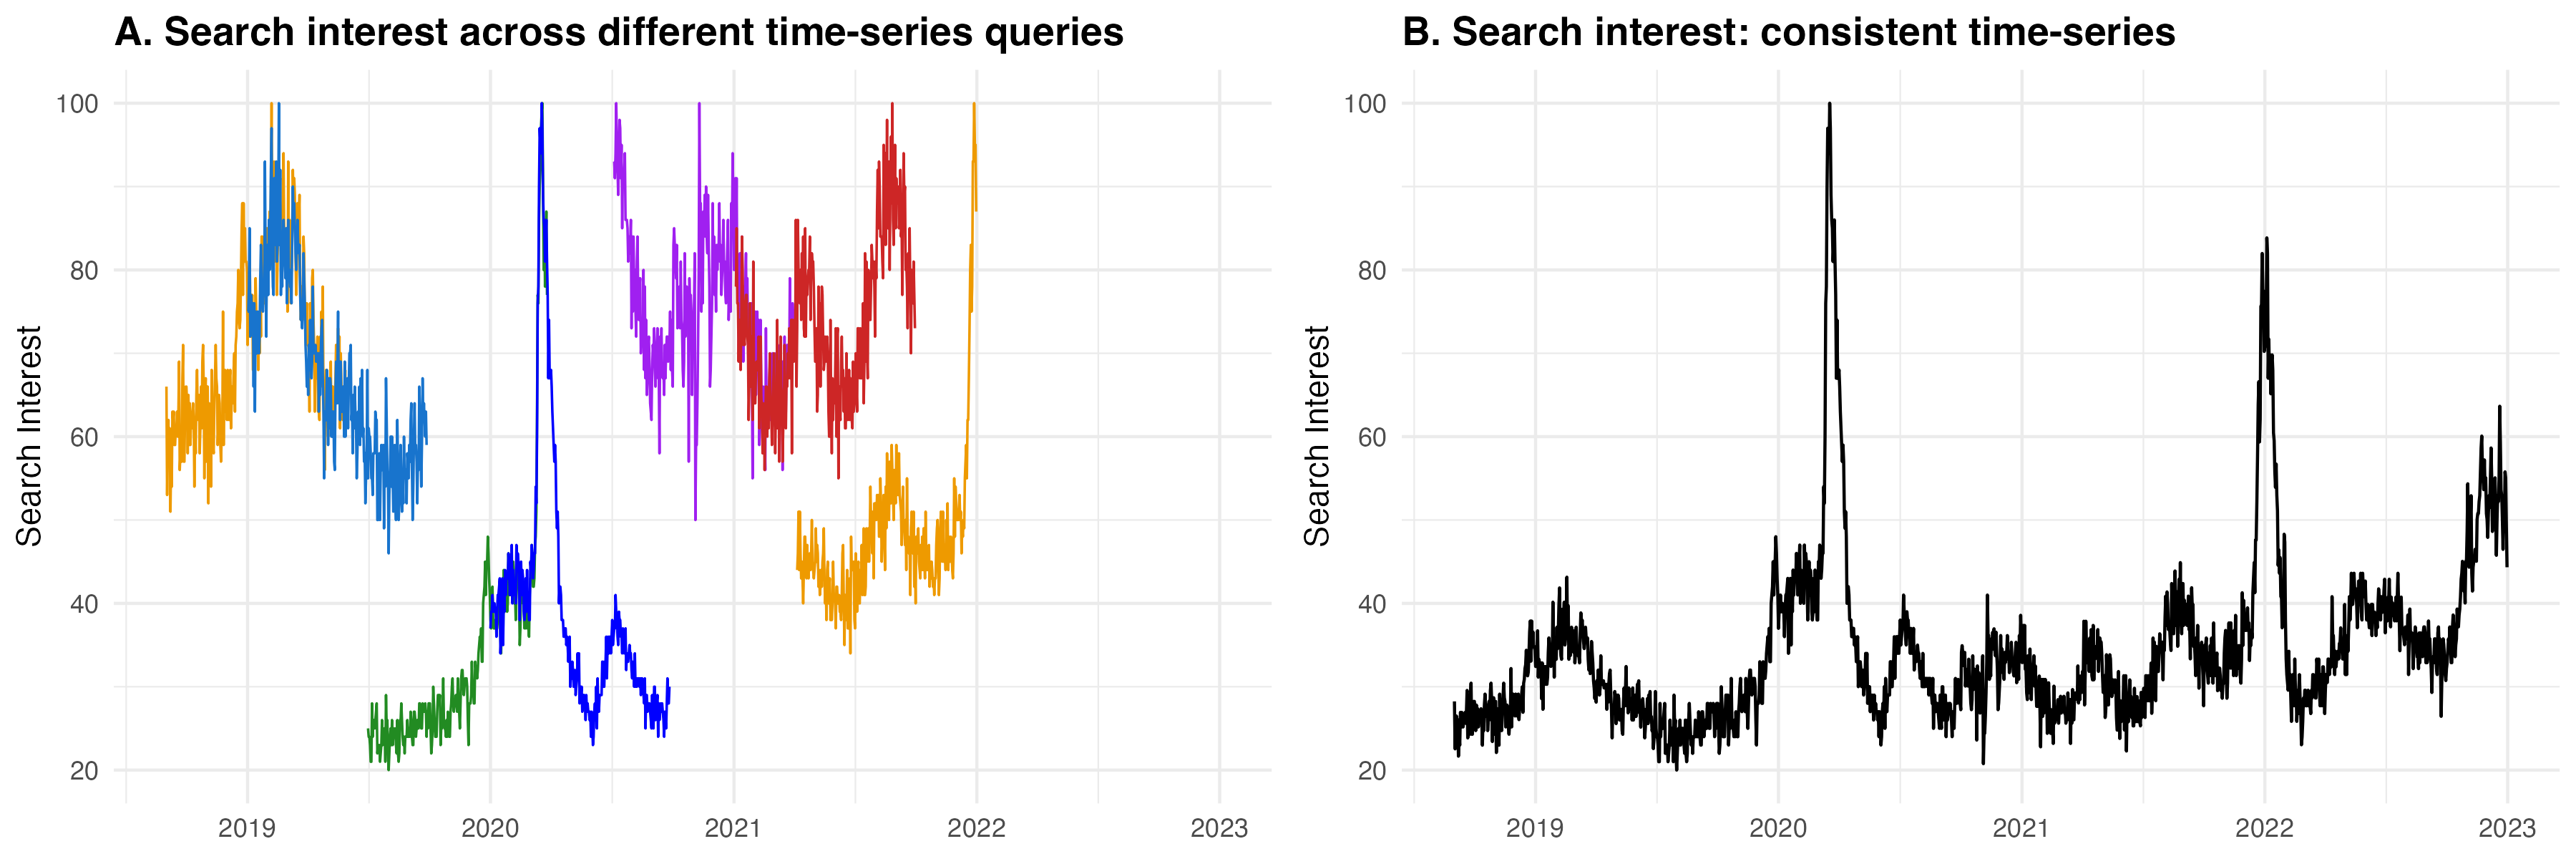
\includegraphics[width=1\textwidth]{figures/const_timeseries_ex.png}
    \caption{Creating a consistent time series of google search interest for search interest in ``fever" for the United States. {\bf Panel A} shows the raw search interest values across queries for search interest across different date ranges. Each query is scaled so its maximum value is 100. {\bf Panel B} shows a consistent time series, creating from scaling values}
    \label{fig:const_timeseries_ex}
\end{figure}

% --------------------------
\newpage
\section{Correlation and lag between search interest and COVID-19 cases}
\label{si:cor_lag_add_results}

\begin{table}[H]
\caption{Correlation between search interest and COVID-19 cases using data in 2020}
\label{tab:cor_table_2020}
\centering
\begin{adjustbox}{width=0.8\textwidth}
\begin{tabular}{l llllllll} 
\hline 
Term & & \multicolumn{5}{c}{Percentile} &  &  \\ 
 & Min & 5th & 25th & 50th & 75th & 95th & Max & N \\ 
\hline 
\multicolumn{9}{l}{{\bf Correlation}} \\ 
Ageusia & -0.17 & -0.08 & -0.02 & 0.03 & 0.1 & 0.24 & 0.32 & 78  \\ 
I Can't Taste & -0.1 & -0.05 & -0.01 & 0.06 & 0.12 & 0.31 & 0.6 & 15  \\ 
How to Treat Coronavirus & -0.29 & -0.2 & -0.06 & -0.02 & 0.09 & 0.23 & 0.34 & 42  \\ 
Anosmia & -0.08 & -0.04 & 0 & 0.06 & 0.14 & 0.28 & 0.43 & 98  \\ 
Shortness of Breath & -0.25 & -0.1 & -0.03 & 0.02 & 0.07 & 0.19 & 0.33 & 128  \\ 
I Can't Smell & -0.07 & -0.06 & -0.01 & 0.08 & 0.16 & 0.32 & 0.42 & 33  \\ 
Cough & -0.46 & -0.24 & -0.07 & -0.01 & 0.05 & 0.17 & 0.36 & 188  \\ 
Pneumonia & -0.37 & -0.18 & -0.05 & -0.02 & 0.06 & 0.33 & 0.63 & 173  \\ 
Fever & -0.46 & -0.28 & -0.06 & -0.01 & 0.06 & 0.18 & 0.41 & 197  \\ 
Loss of Taste & -0.05 & -0.04 & 0.05 & 0.13 & 0.25 & 0.6 & 0.83 & 99  \\ 
Loss of Smell & -0.06 & -0.04 & 0.06 & 0.17 & 0.33 & 0.64 & 0.81 & 104  \\ 
Covid-19 & -0.3 & -0.13 & -0.03 & 0.02 & 0.11 & 0.26 & 0.7 & 205  \\ 
Coronavirus & -0.49 & -0.39 & -0.24 & -0.12 & -0.03 & 0.16 & 0.59 & 207  \\ 
Covid Symptoms & -0.08 & -0.04 & 0.02 & 0.11 & 0.3 & 0.62 & 0.72 & 136  \\ 
\hline 
\multicolumn{9}{l}{{\bf Correlation using best lag}} \\ 
Ageusia & -0.12 & -0.05 & 0.02 & 0.12 & 0.2 & 0.35 & 0.53 & 78  \\ 
I Can't Taste & -0.06 & 0.01 & 0.08 & 0.1 & 0.2 & 0.35 & 0.6 & 15  \\ 
How to Treat Coronavirus & -0.22 & -0.16 & -0.03 & 0.05 & 0.23 & 0.4 & 0.51 & 42  \\ 
Anosmia & -0.05 & -0.02 & 0.07 & 0.16 & 0.24 & 0.43 & 0.52 & 98  \\ 
Shortness of Breath & -0.15 & -0.05 & 0.03 & 0.1 & 0.16 & 0.31 & 0.49 & 128  \\ 
I Can't Smell & -0.06 & -0.04 & 0.06 & 0.13 & 0.26 & 0.41 & 0.55 & 33  \\ 
Cough & -0.41 & -0.19 & -0.03 & 0.06 & 0.13 & 0.29 & 0.45 & 188  \\ 
Pneumonia & -0.35 & -0.13 & -0.01 & 0.08 & 0.19 & 0.4 & 0.74 & 173  \\ 
Fever & -0.37 & -0.2 & 0 & 0.08 & 0.17 & 0.33 & 0.73 & 197  \\ 
Loss of Taste & -0.04 & -0.01 & 0.11 & 0.25 & 0.37 & 0.66 & 0.86 & 99  \\ 
Loss of Smell & -0.06 & -0.02 & 0.17 & 0.28 & 0.43 & 0.68 & 0.88 & 104  \\ 
Covid-19 & -0.26 & -0.06 & 0.04 & 0.15 & 0.22 & 0.47 & 0.75 & 205  \\ 
Coronavirus & -0.47 & -0.35 & -0.17 & -0.05 & 0.07 & 0.39 & 0.76 & 207  \\ 
Covid Symptoms & -0.06 & -0.01 & 0.14 & 0.24 & 0.41 & 0.69 & 0.9 & 136  \\ 
\hline 
\multicolumn{9}{l}{{\bf Lag with best correlation}} \\ 
Ageusia & -21 & -21 & -17.75 & -10.5 & 5 & 21 & 21 & 78  \\ 
I Can't Taste & -21 & -20.3 & -18.5 & -16 & 0 & 20.3 & 21 & 15  \\ 
How to Treat Coronavirus & -21 & -20.95 & -19 & -16 & -10 & 0.9 & 13 & 42  \\ 
Anosmia & -21 & -21 & -17 & -11 & -4.25 & 18.3 & 21 & 98  \\ 
Shortness of Breath & -21 & -20 & -16 & -6 & 7.25 & 17 & 21 & 128  \\ 
I Can't Smell & -20 & -20 & -16 & -8 & 2 & 18.4 & 21 & 33  \\ 
Cough & -21 & -21 & -14.25 & -6.5 & 4.25 & 20 & 21 & 188  \\ 
Pneumonia & -21 & -21 & -15 & -6 & 6 & 19 & 21 & 173  \\ 
Fever & -21 & -21 & -16 & -7 & 4 & 19.2 & 21 & 197  \\ 
Loss of Taste & -21 & -21 & -18 & -11 & -3.5 & 13.4 & 20 & 99  \\ 
Loss of Smell & -21 & -21 & -18.25 & -11 & -2 & 16.85 & 21 & 104  \\ 
Covid-19 & -21 & -21 & -18 & -11 & -4 & 13.8 & 21 & 205  \\ 
Coronavirus & -21 & -21 & -21 & -16 & -9 & 3 & 21 & 207  \\ 
Covid Symptoms & -21 & -21 & -17 & -10.5 & -3.75 & 13.25 & 20 & 136  \\ 
\hline 
\end{tabular} 
\end{adjustbox}
\end{table}

\begin{table}[H]
\caption{Correlation between search interest and COVID-19 cases using data in 2021}
\label{tab:cor_table_2021}
\centering
\begin{adjustbox}{width=0.8\textwidth}
\begin{tabular}{l llllllll} 
\hline 
Term & & \multicolumn{5}{c}{Percentile} &  &  \\ 
 & Min & 5th & 25th & 50th & 75th & 95th & Max & N \\ 
\hline 
\multicolumn{9}{l}{{\bf Correlation}}  \\ 
Ageusia & -0.22 & -0.09 & -0.03 & 0.02 & 0.09 & 0.19 & 0.34 & 76  \\ 
I Can't Taste & -0.06 & -0.05 & -0.01 & 0.07 & 0.15 & 0.26 & 0.26 & 17  \\ 
How to Treat Coronavirus & -0.21 & -0.16 & -0.05 & 0.08 & 0.17 & 0.29 & 0.32 & 58  \\ 
Anosmia & -0.11 & -0.06 & 0 & 0.04 & 0.13 & 0.26 & 0.52 & 100  \\ 
Shortness of Breath & -0.15 & -0.07 & -0.02 & 0.04 & 0.12 & 0.36 & 0.87 & 123  \\ 
I Can't Smell & -0.19 & -0.11 & -0.01 & 0.03 & 0.09 & 0.25 & 0.55 & 31  \\ 
Cough & -0.47 & -0.08 & -0.01 & 0.06 & 0.15 & 0.39 & 0.9 & 188  \\ 
Pneumonia & -0.19 & -0.07 & -0.01 & 0.05 & 0.15 & 0.44 & 0.94 & 168  \\ 
Fever & -0.18 & -0.07 & -0.01 & 0.05 & 0.14 & 0.51 & 0.88 & 201  \\ 
Loss of Taste & -0.15 & -0.05 & 0.02 & 0.09 & 0.17 & 0.43 & 0.82 & 99  \\ 
Loss of Smell & -0.05 & -0.03 & 0.03 & 0.09 & 0.2 & 0.47 & 0.86 & 104  \\ 
Covid-19 & -0.16 & -0.06 & 0 & 0.07 & 0.18 & 0.4 & 0.65 & 202  \\ 
Coronavirus & -0.28 & -0.1 & -0.01 & 0.05 & 0.24 & 0.56 & 0.81 & 211  \\ 
Covid Symptoms & -0.11 & -0.05 & 0.04 & 0.13 & 0.29 & 0.67 & 0.94 & 138  \\ 
\hline 
\multicolumn{9}{l}{{\bf Correlation using best lag}}  \\ 
Ageusia & -0.17 & -0.01 & 0.03 & 0.1 & 0.18 & 0.36 & 0.48 & 76  \\ 
I Can't Taste & 0 & 0.01 & 0.09 & 0.14 & 0.24 & 0.29 & 0.39 & 17  \\ 
How to Treat Coronavirus & -0.18 & -0.14 & 0.04 & 0.14 & 0.27 & 0.34 & 0.51 & 58  \\ 
Anosmia & -0.09 & -0.03 & 0.08 & 0.13 & 0.22 & 0.34 & 0.56 & 100  \\ 
Shortness of Breath & -0.09 & -0.03 & 0.07 & 0.13 & 0.21 & 0.43 & 0.88 & 123  \\ 
I Can't Smell & -0.1 & -0.06 & 0.1 & 0.13 & 0.18 & 0.29 & 0.71 & 31  \\ 
Cough & -0.38 & -0.03 & 0.08 & 0.15 & 0.24 & 0.53 & 0.92 & 188  \\ 
Pneumonia & -0.16 & -0.01 & 0.08 & 0.16 & 0.25 & 0.57 & 0.95 & 168  \\ 
Fever & -0.16 & -0.01 & 0.09 & 0.14 & 0.24 & 0.62 & 0.91 & 201  \\ 
Loss of Taste & -0.07 & 0 & 0.1 & 0.16 & 0.25 & 0.51 & 0.9 & 99  \\ 
Loss of Smell & -0.02 & 0.02 & 0.11 & 0.2 & 0.28 & 0.56 & 0.94 & 104  \\ 
Covid-19 & -0.08 & -0.01 & 0.1 & 0.17 & 0.29 & 0.51 & 0.76 & 202  \\ 
Coronavirus & -0.21 & -0.03 & 0.09 & 0.18 & 0.33 & 0.61 & 0.87 & 211  \\ 
Covid Symptoms & -0.09 & 0.02 & 0.17 & 0.24 & 0.4 & 0.74 & 0.98 & 138  \\ 
\hline 
\multicolumn{9}{l}{{\bf Lag with best correlation}}  \\ 
Ageusia & -21 & -21 & -15.25 & 0 & 17.25 & 21 & 21 & 76  \\ 
I Can't Taste & -21 & -19.4 & -16 & -9 & 3 & 17 & 21 & 17  \\ 
How to Treat Coronavirus & -21 & -21 & -17.75 & -11 & 2 & 20.15 & 21 & 58  \\ 
Anosmia & -21 & -21 & -16 & -4 & 12 & 20 & 21 & 100  \\ 
Shortness of Breath & -21 & -20 & -10 & 1 & 13 & 20 & 21 & 123  \\ 
I Can't Smell & -21 & -21 & -17.5 & -5 & 12.5 & 21 & 21 & 31  \\ 
Cough & -21 & -21 & -13 & -4 & 3 & 19 & 21 & 188  \\ 
Pneumonia & -21 & -19 & -11 & -2 & 10 & 21 & 21 & 168  \\ 
Fever & -21 & -20 & -12 & -3 & 7 & 20 & 21 & 201  \\ 
Loss of Taste & -21 & -20 & -11 & -3 & 8.5 & 19.1 & 21 & 99  \\ 
Loss of Smell & -21 & -20 & -14 & -6 & 3 & 16.85 & 21 & 104  \\ 
Covid-19 & -21 & -19 & -12 & -2 & 7 & 19.95 & 21 & 202  \\ 
Coronavirus & -21 & -20 & -9 & -1 & 10 & 20.5 & 21 & 211  \\ 
Covid Symptoms & -21 & -17 & -10.75 & -4 & 1.75 & 18.15 & 21 & 138  \\ 
\hline 
\end{tabular} 
\end{adjustbox}
\end{table}

\begin{table}[H]
\caption{Correlation between search interest and COVID-19 cases using data in 2022}
\label{tab:cor_table_2022}
\centering
\begin{adjustbox}{width=0.8\textwidth}
\begin{tabular}{l llllllll} 
\hline 
Term & & \multicolumn{5}{c}{Percentile} &  &  \\ 
 & Min & 5th & 25th & 50th & 75th & 95th & Max & N \\ 
\hline 
\multicolumn{9}{l}{{\bf Correlation}} \\ 
Ageusia & -0.11 & -0.09 & -0.04 & 0.02 & 0.07 & 0.15 & 0.28 & 62  \\ 
I Can't Taste & -0.11 & -0.11 & -0.01 & 0.02 & 0.06 & 0.23 & 0.39 & 14  \\ 
How to Treat Coronavirus & -0.13 & -0.04 & 0 & 0.04 & 0.11 & 0.16 & 0.26 & 48  \\ 
Anosmia & -0.1 & -0.07 & -0.02 & 0.03 & 0.11 & 0.26 & 0.49 & 89  \\ 
Shortness of Breath & -0.14 & -0.08 & -0.03 & 0.03 & 0.11 & 0.29 & 0.54 & 115  \\ 
I Can't Smell & -0.06 & -0.05 & -0.02 & 0.02 & 0.07 & 0.34 & 0.42 & 23  \\ 
Cough & -0.29 & -0.08 & -0.01 & 0.05 & 0.13 & 0.47 & 0.77 & 187  \\ 
Pneumonia & -0.21 & -0.09 & -0.03 & 0.02 & 0.09 & 0.26 & 0.55 & 158  \\ 
Fever & -0.25 & -0.08 & -0.02 & 0.04 & 0.13 & 0.47 & 0.78 & 196  \\ 
Loss of Taste & -0.1 & -0.08 & 0 & 0.06 & 0.11 & 0.33 & 0.78 & 80  \\ 
Loss of Smell & -0.09 & -0.05 & -0.01 & 0.03 & 0.12 & 0.4 & 0.72 & 85  \\ 
Covid-19 & -0.24 & -0.05 & 0.02 & 0.13 & 0.34 & 0.71 & 0.91 & 198  \\ 
Coronavirus & -0.2 & -0.06 & 0.02 & 0.13 & 0.45 & 0.76 & 0.92 & 198  \\ 
Covid Symptoms & -0.1 & -0.06 & 0 & 0.1 & 0.27 & 0.74 & 0.86 & 138  \\ 
\hline 
\multicolumn{9}{l}{{\bf Correlation using best lag}}  \\ 
Ageusia & -0.09 & -0.03 & 0.04 & 0.09 & 0.16 & 0.26 & 0.3 & 62  \\ 
I Can't Taste & -0.07 & -0.02 & 0.04 & 0.1 & 0.16 & 0.27 & 0.43 & 14  \\ 
How to Treat Coronavirus & 0.02 & 0.04 & 0.07 & 0.14 & 0.18 & 0.26 & 0.38 & 48  \\ 
Anosmia & -0.03 & 0.01 & 0.07 & 0.14 & 0.22 & 0.35 & 0.57 & 89  \\ 
Shortness of Breath & -0.13 & 0.02 & 0.08 & 0.13 & 0.21 & 0.37 & 0.65 & 115  \\ 
I Can't Smell & -0.01 & 0 & 0.09 & 0.13 & 0.18 & 0.41 & 0.43 & 23  \\ 
Cough & -0.25 & -0.03 & 0.08 & 0.15 & 0.26 & 0.61 & 0.88 & 187  \\ 
Pneumonia & -0.17 & -0.01 & 0.08 & 0.14 & 0.2 & 0.38 & 0.75 & 158  \\ 
Fever & -0.19 & 0.01 & 0.09 & 0.15 & 0.26 & 0.64 & 0.89 & 196  \\ 
Loss of Taste & -0.07 & 0 & 0.08 & 0.13 & 0.18 & 0.49 & 0.85 & 80  \\ 
Loss of Smell & -0.02 & 0.01 & 0.08 & 0.12 & 0.22 & 0.48 & 0.83 & 85  \\ 
Covid-19 & -0.19 & 0.07 & 0.13 & 0.24 & 0.45 & 0.83 & 0.92 & 198  \\ 
Coronavirus & -0.19 & 0.06 & 0.15 & 0.23 & 0.51 & 0.84 & 0.93 & 198  \\ 
Covid Symptoms & -0.03 & 0.04 & 0.12 & 0.22 & 0.4 & 0.85 & 0.97 & 138  \\ 
\hline 
\multicolumn{9}{l}{{\bf Lag with best correlation}} \\ 
Ageusia & -21 & -21 & -13.5 & 0 & 11 & 20 & 21 & 62  \\ 
I Can't Taste & -21 & -19.05 & -7.25 & -4 & 6.5 & 16.75 & 20 & 14  \\ 
How to Treat Coronavirus & -21 & -20.65 & -13.5 & 0 & 8.5 & 16 & 21 & 48  \\ 
Anosmia & -21 & -21 & -13 & -5 & 5 & 19.6 & 21 & 89  \\ 
Shortness of Breath & -21 & -20 & -12 & 0 & 12 & 20 & 21 & 115  \\ 
I Can't Smell & -21 & -21 & -17 & -7 & 8 & 16.9 & 20 & 23  \\ 
Cough & -21 & -21 & -15 & -6 & 4 & 18 & 21 & 187  \\ 
Pneumonia & -21 & -21 & -16 & -3 & 11 & 20 & 21 & 158  \\ 
Fever & -21 & -20 & -15 & -8 & 4 & 19.25 & 21 & 196  \\ 
Loss of Taste & -21 & -21 & -15 & -6.5 & 5.25 & 18.05 & 21 & 80  \\ 
Loss of Smell & -20 & -18.8 & -12 & -3 & 11 & 18 & 21 & 85  \\ 
Covid-19 & -21 & -19 & -14 & -5 & 5 & 17.15 & 21 & 198  \\ 
Coronavirus & -21 & -21 & -15 & -8 & 0 & 16 & 21 & 198  \\ 
Covid Symptoms & -21 & -20 & -13 & -5 & 3.75 & 17.15 & 21 & 138  \\ 
\hline 
\end{tabular} 
\end{adjustbox}
\end{table}

\begin{figure}[H]
    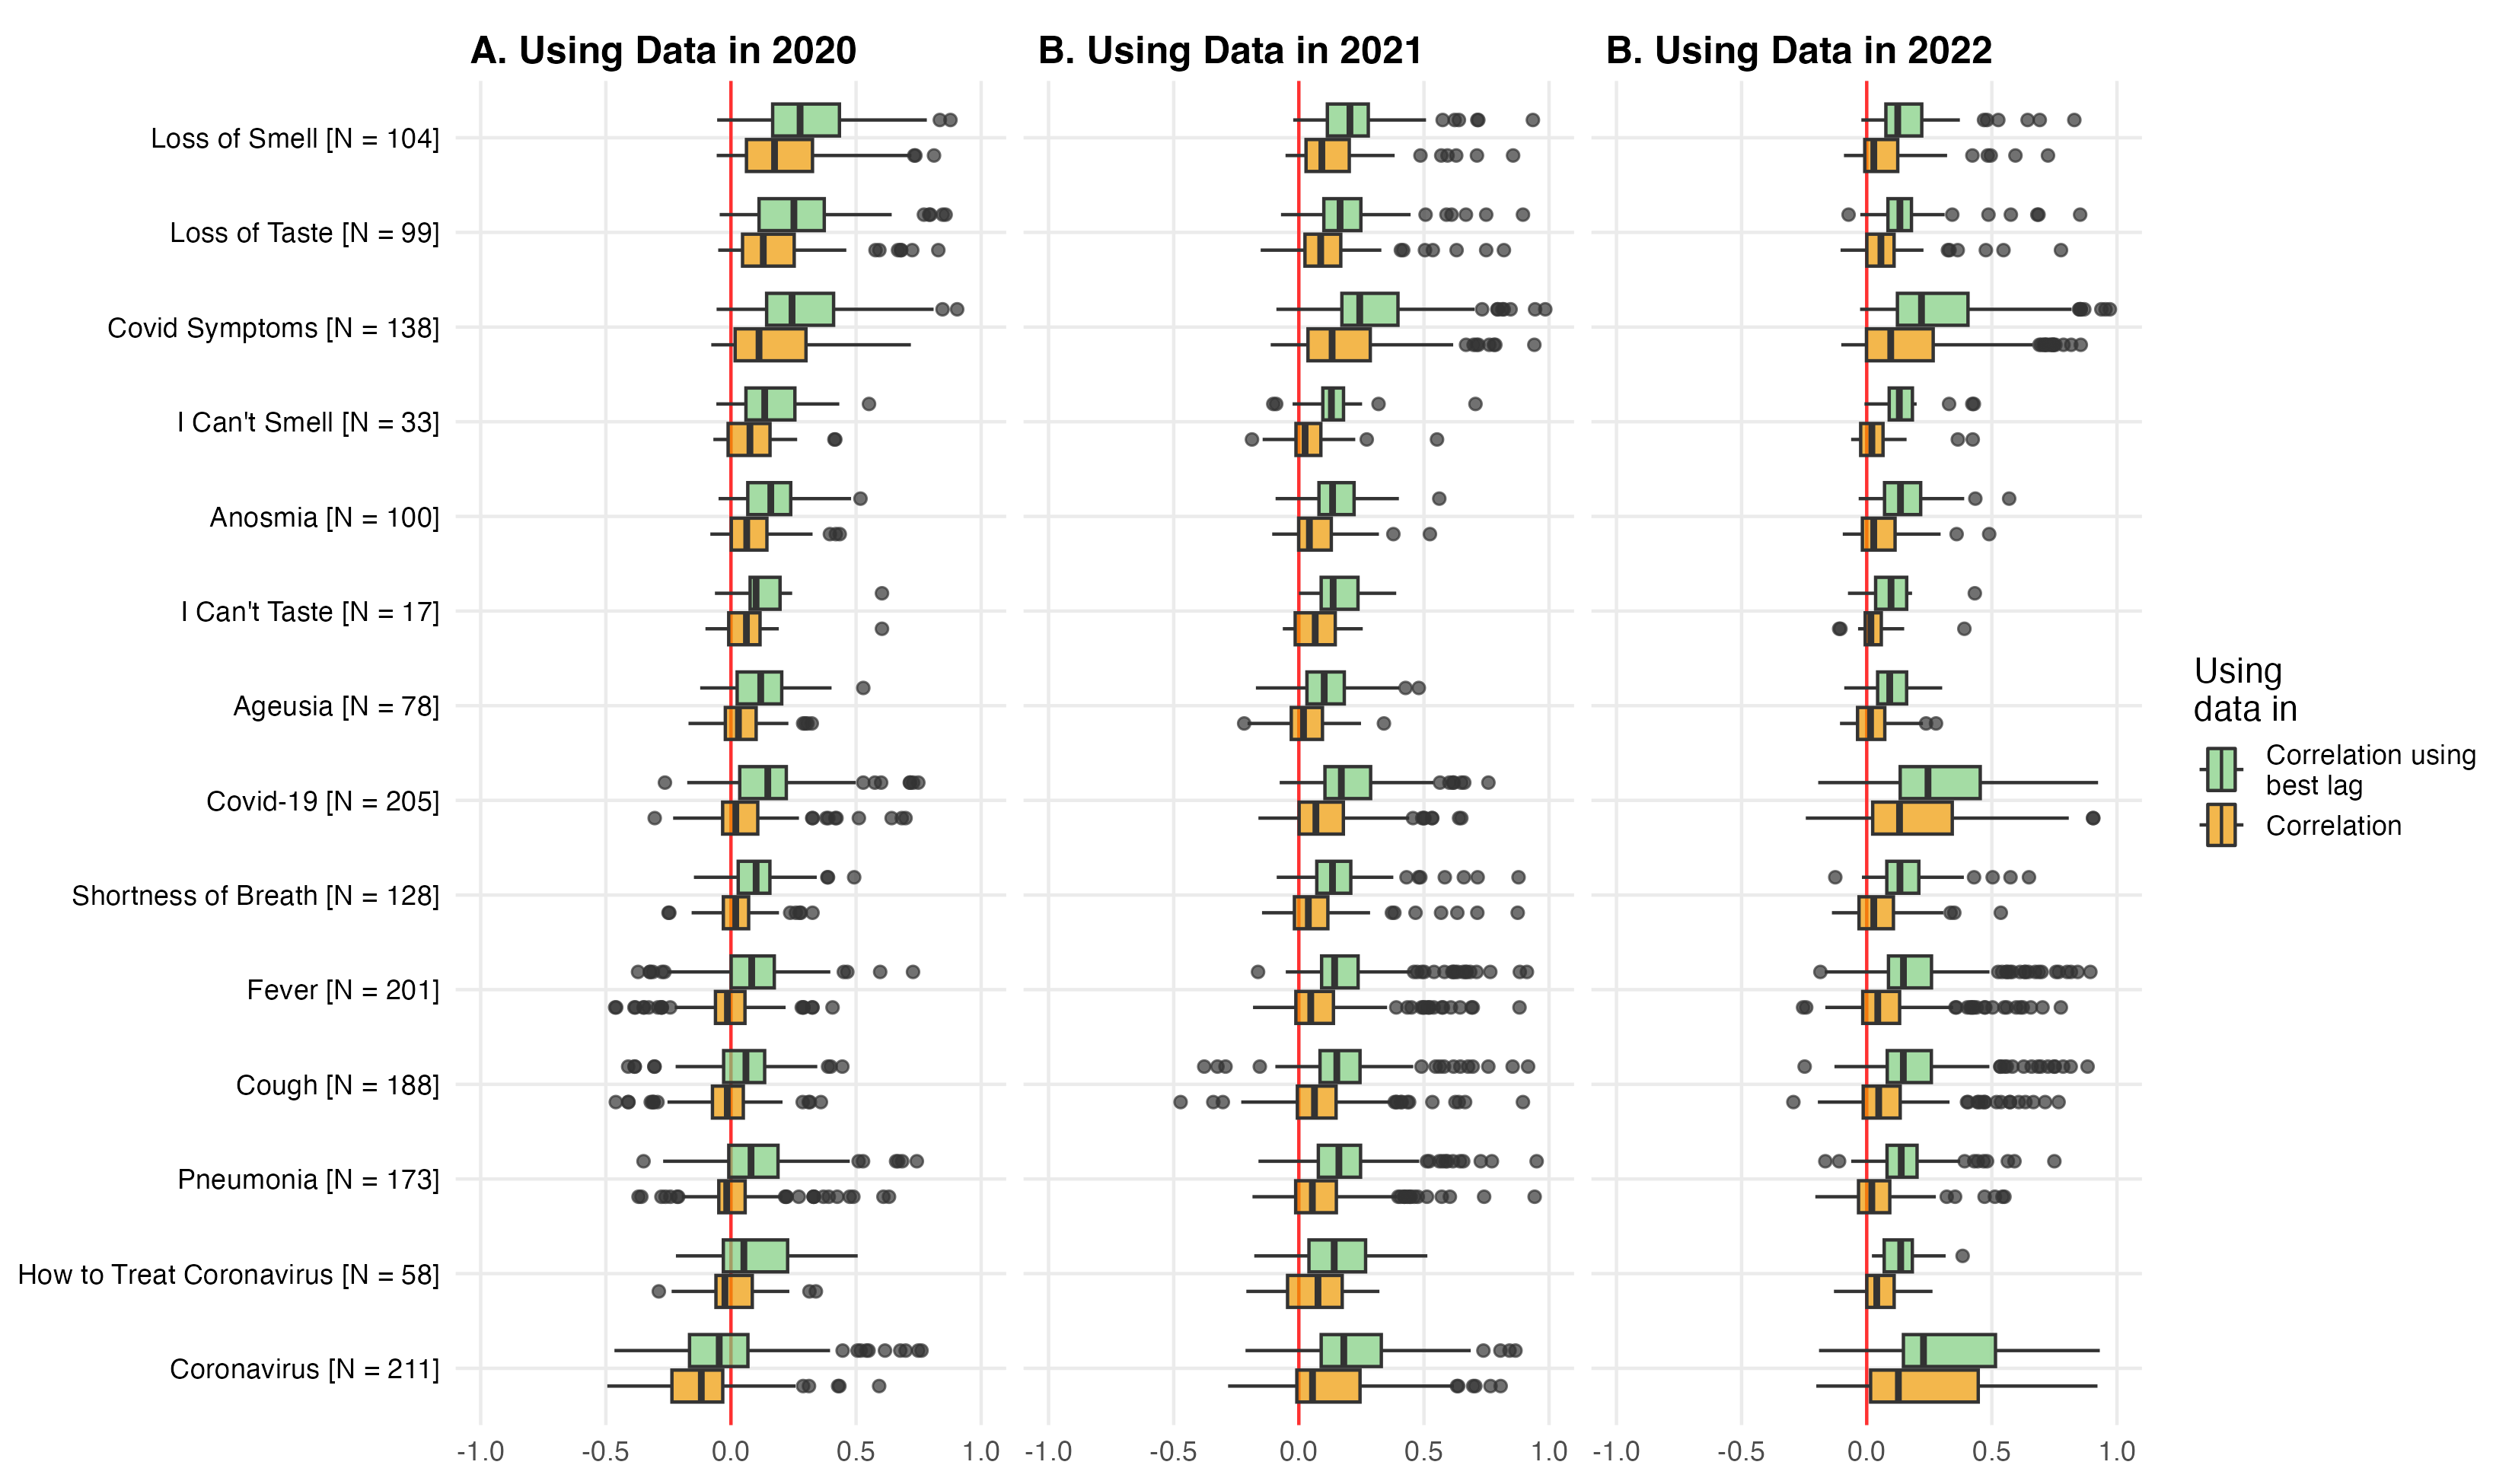
\includegraphics[width=1\textwidth]{figures/cor_corbest_fig.png}
    \caption{Distribution of correlation between search interest and COVID-19 cases using the original correlation and the correlation when using the lagged value of COVID-19 cases that produced the highest correlation. `N' indicates the number of countries with available data. The boxplots include: center line, median; box limits, upper and lower quartiles; whiskers, 1.5x interquartile range; points beyond whiskers, outliers.}
    \label{fig:cor_best}
\end{figure}

% --------------------------
\newpage
\section{Map of correlations of search interest in ``Loss of Smell'' and ``Fever'' with COVID-19 cases}
\label{si:cor_map}

% trim={<left> <lower> <right> <upper>}
\begin{figure}[H]
    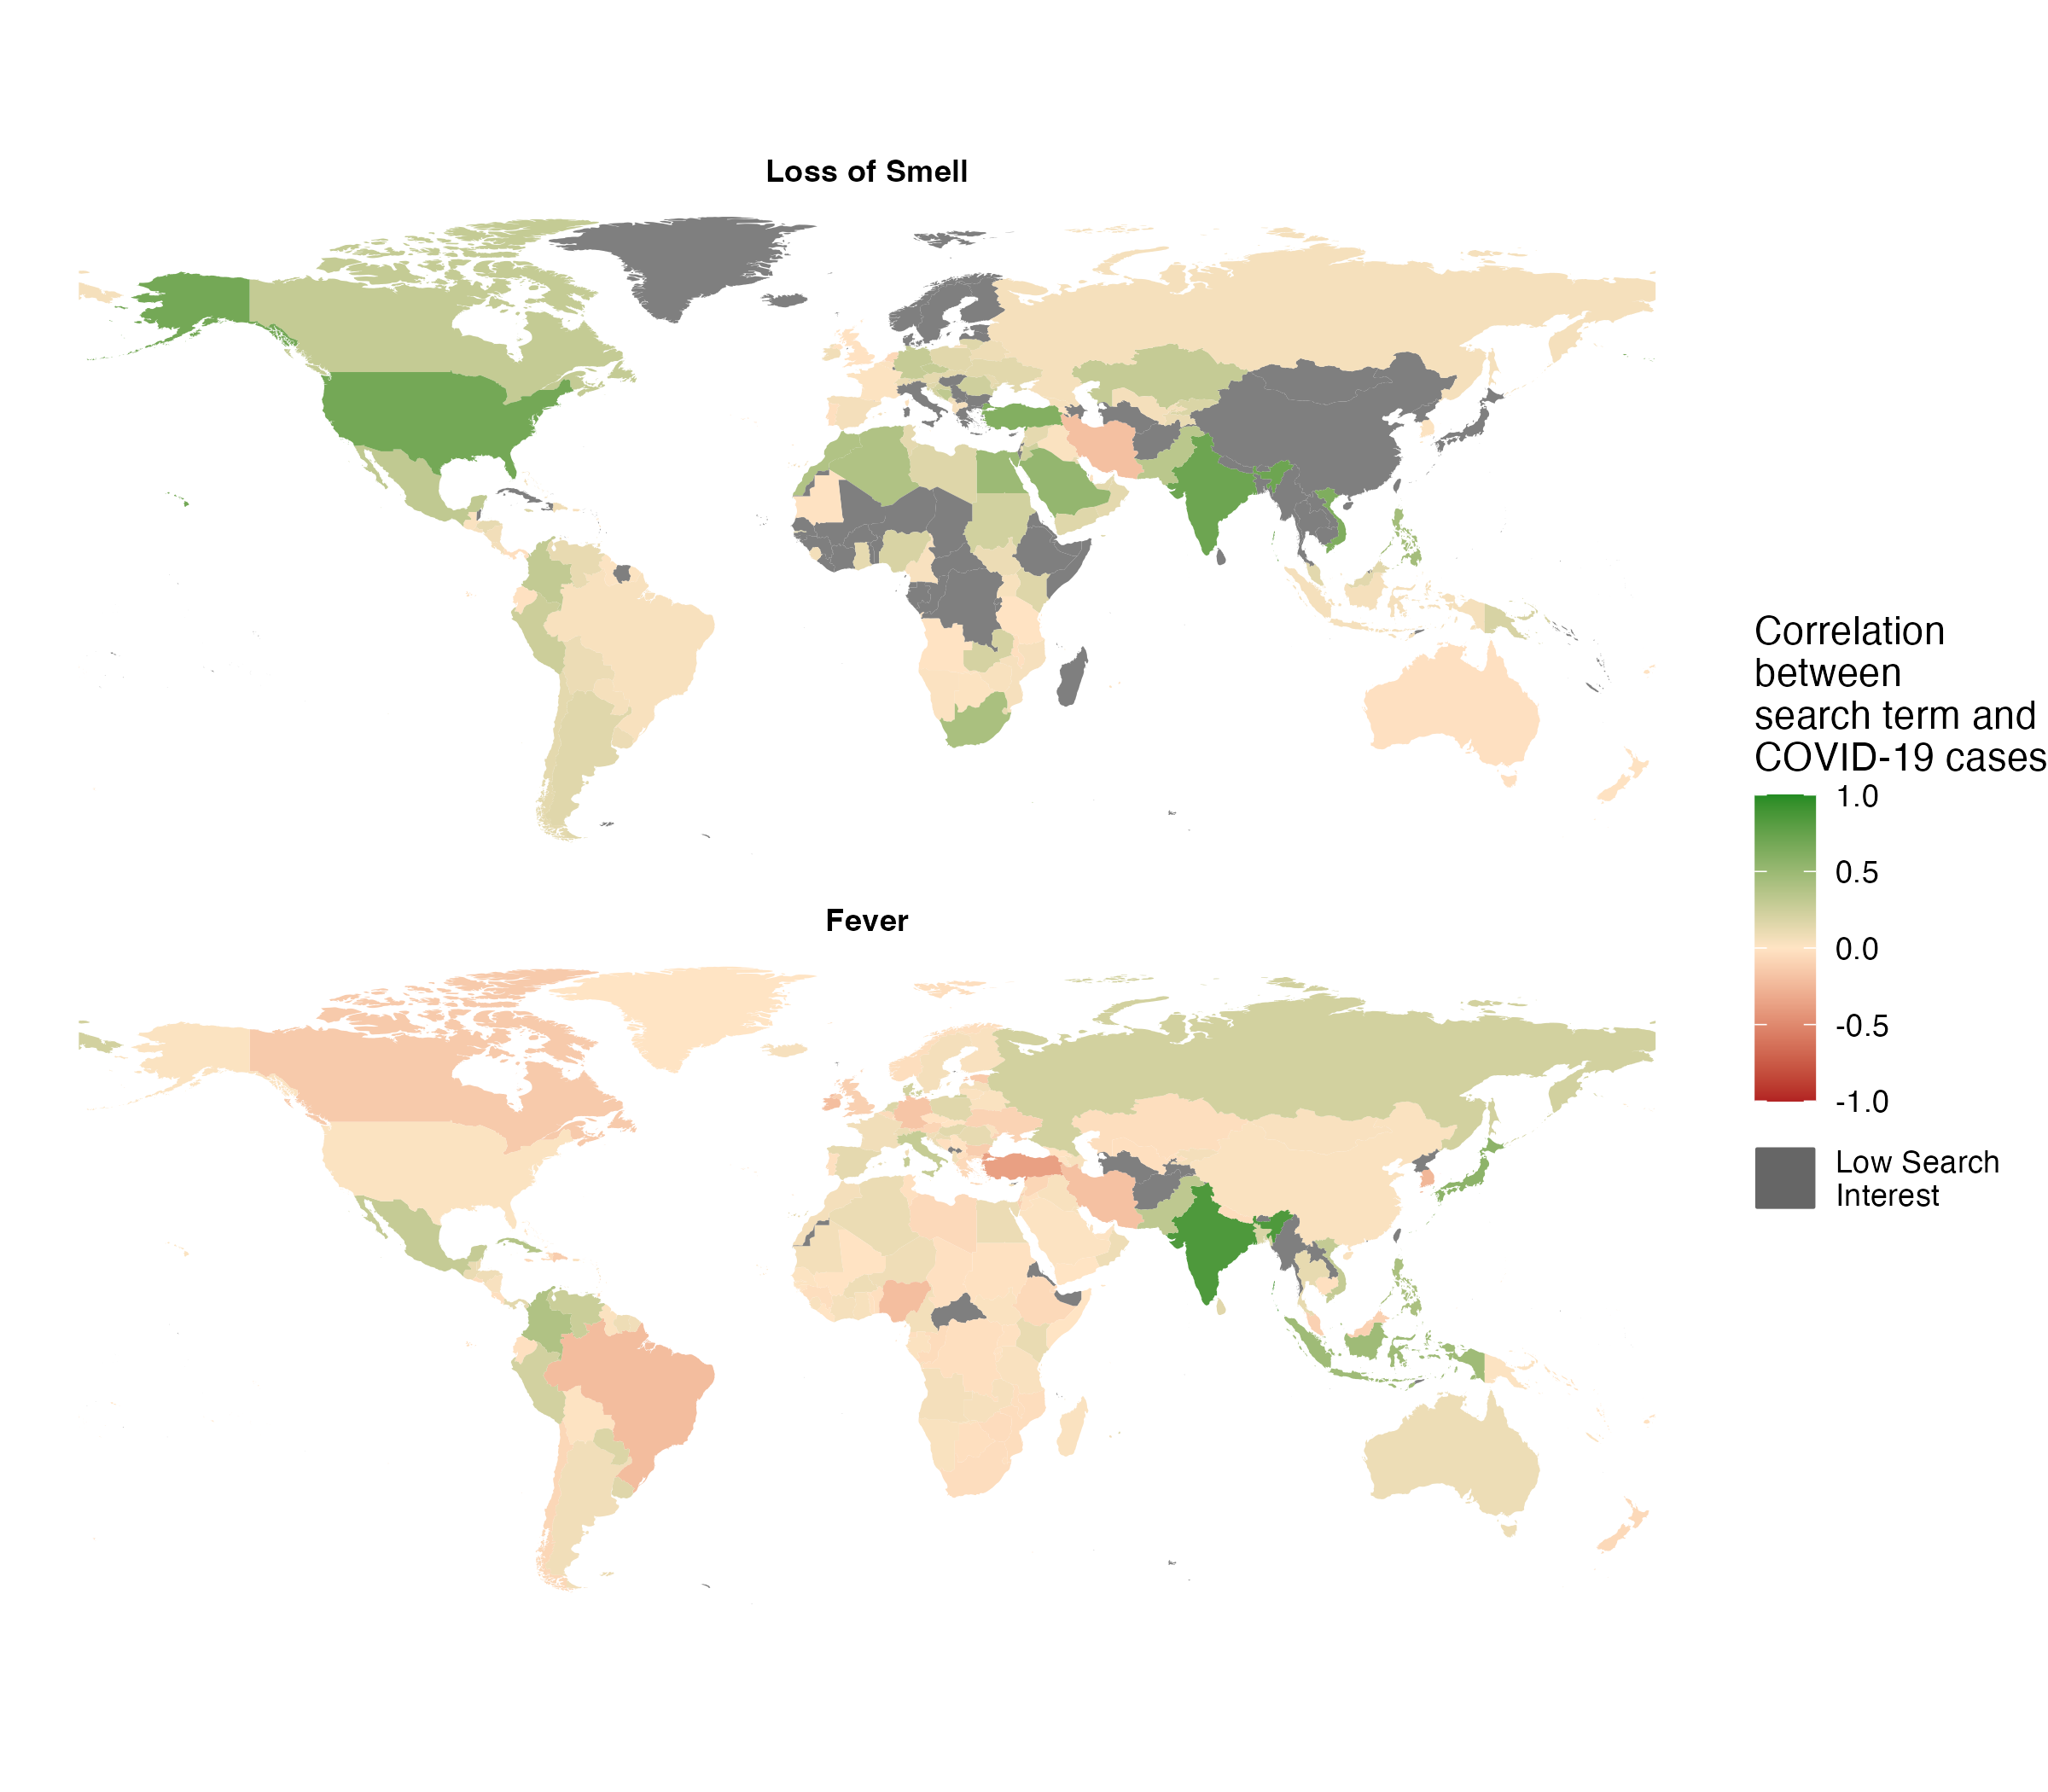
\includegraphics[width=1\textwidth]{figures/cor_map.png} % trim={0 1m 0 0},clip]
    \caption{Correlation between reported COVID-19 cases and search interest in ``Loss of Smell'' and ``Fever.'' Maps produced using R, version 4.2.2 (\url{https://www.r-project.org/}); data for country boundaries come from Natural Earth (\url{https://www.naturalearthdata.com/}).}
    \label{fig:cor_world_map}
\end{figure}

% --------------------------
\newpage
\section{Trends in search interest for ``Loss of Smell'' and COVID-19 cases for all countries with available data}
\label{si:lossofsmell_covid_allcountries}

\begin{figure}[H]
    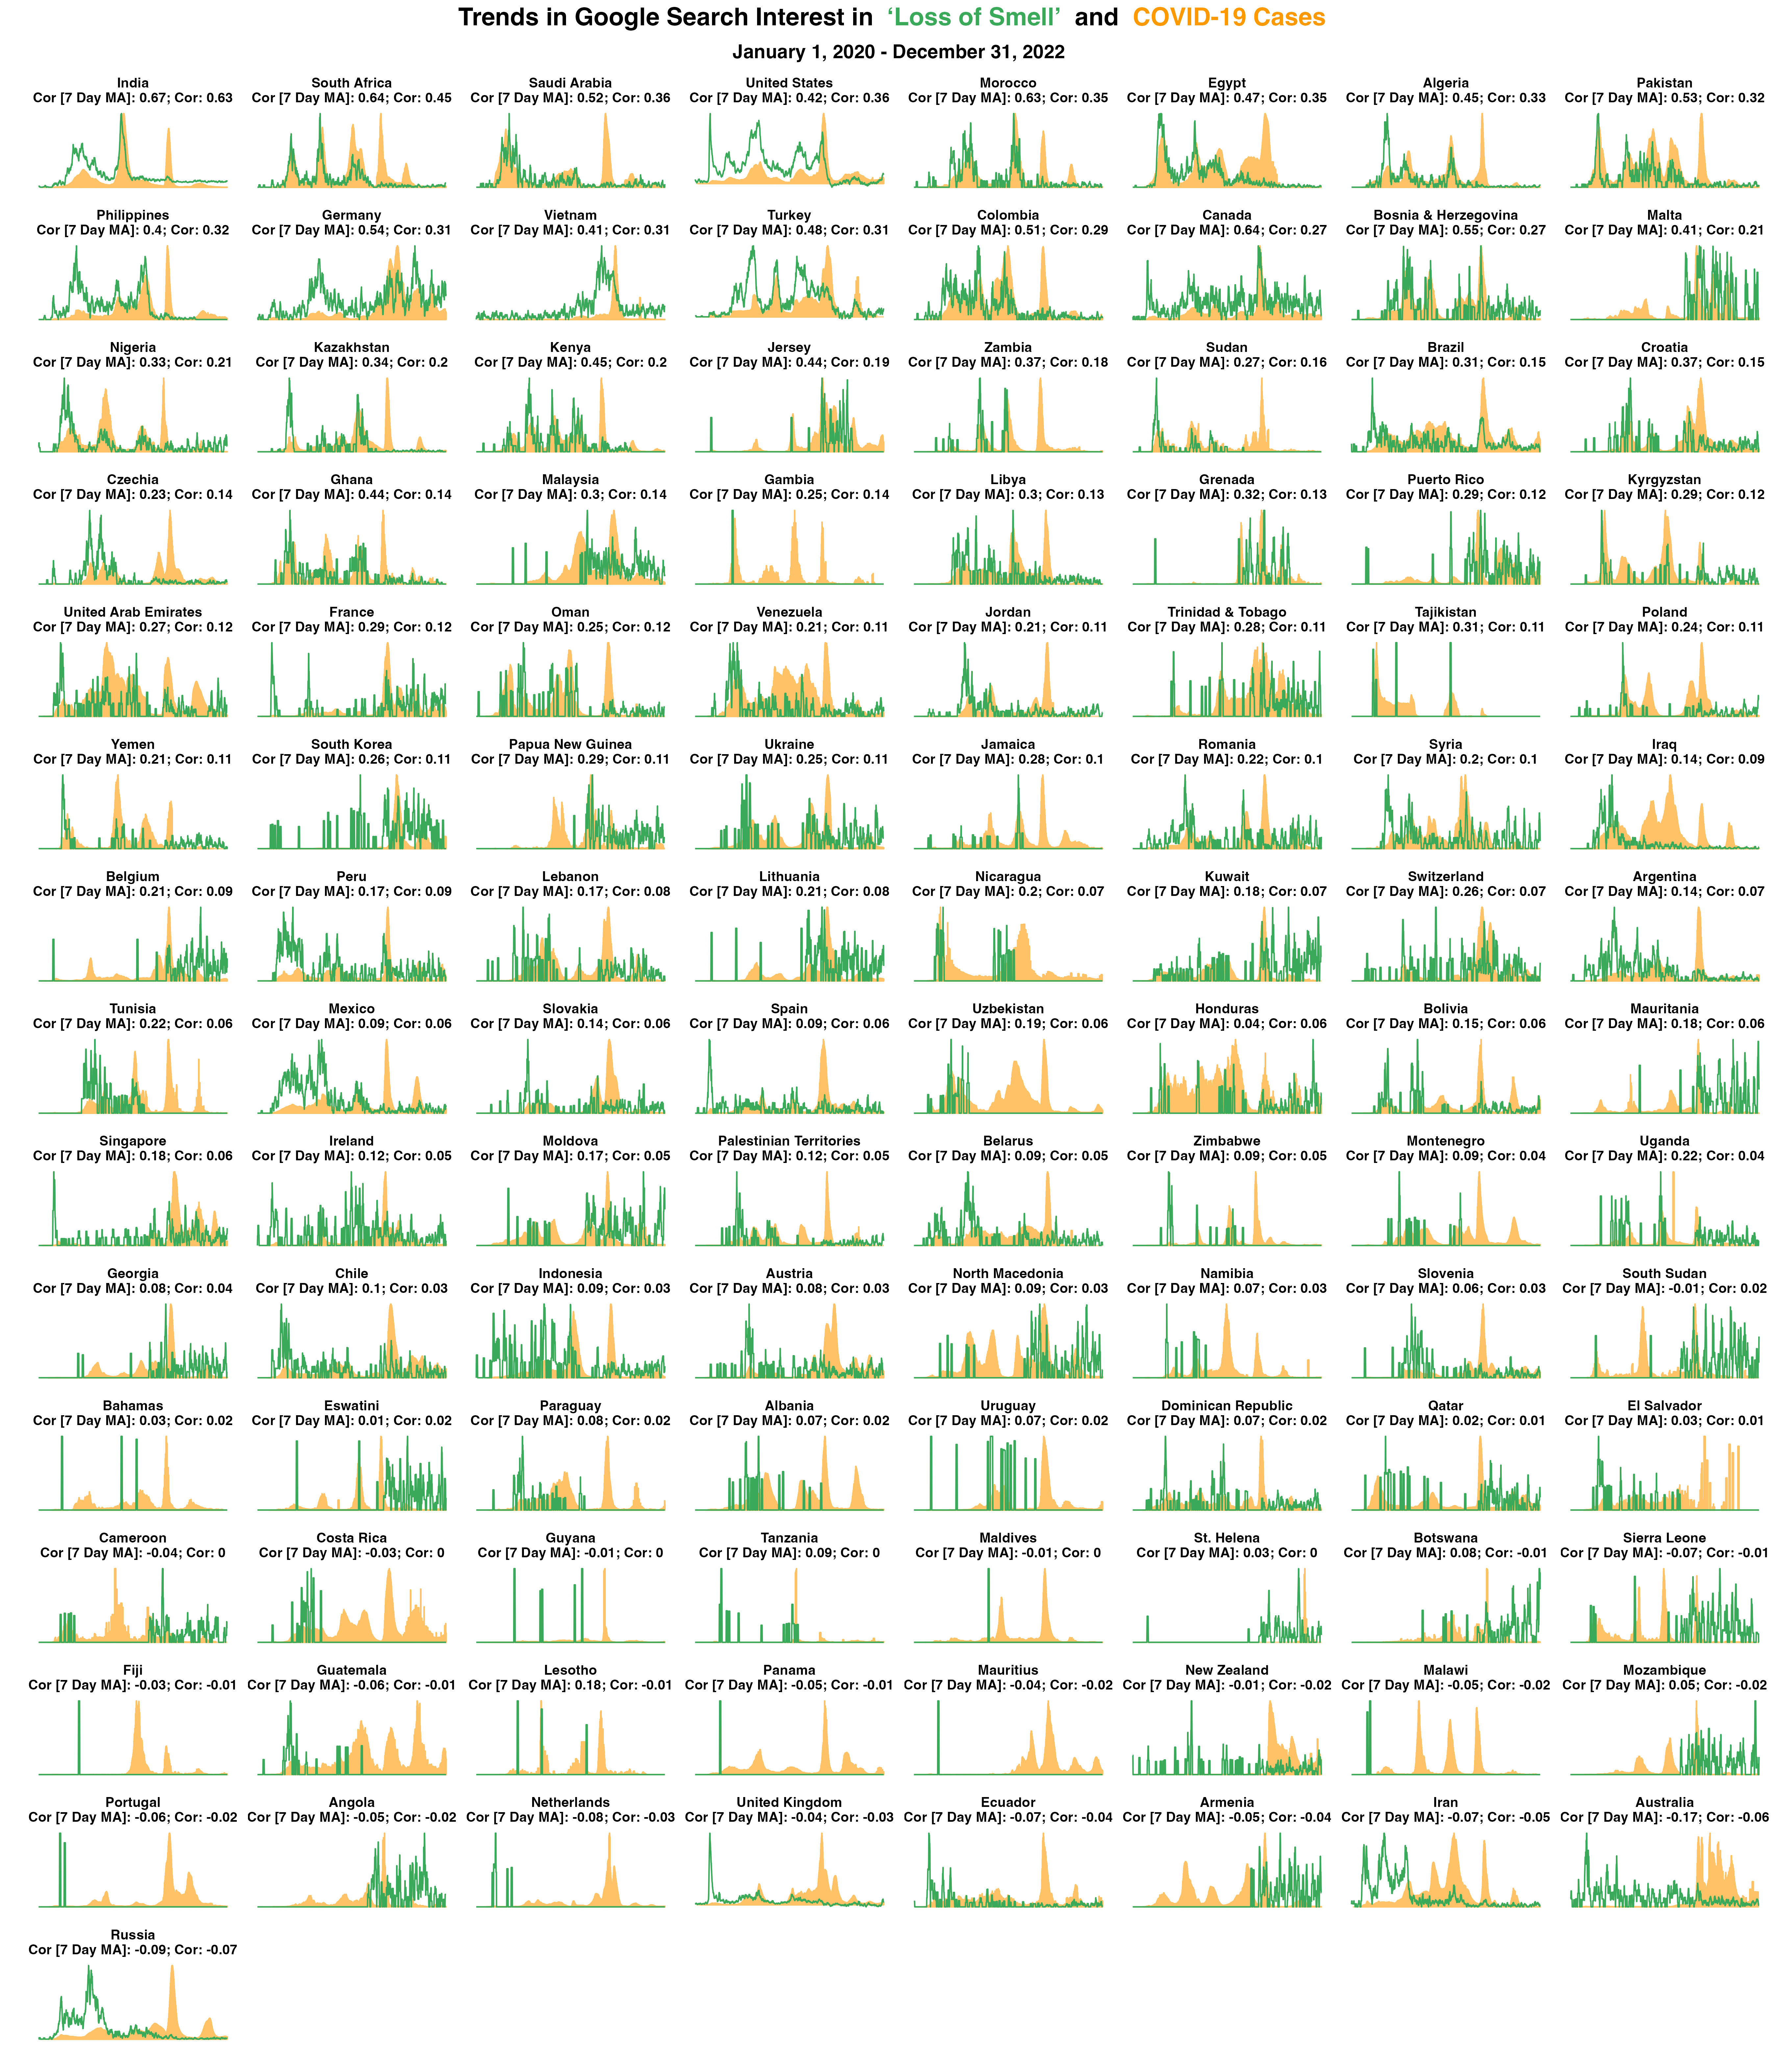
\includegraphics[width=1\textwidth]{figures/cases_vs_loss_of_smell_trends_allcountries.png}
    \caption{Trends between search interest in ``Loss of Smell'' and COVID-19 cases for all countries with available data. To show trends more clearly, the seven-day moving average of search interest is shown.}
    \label{fig:cases_vs_loss_of_smell_trends_allcountries}
\end{figure}

% --------------------------
\newpage
\section{Trends in search interest for ``COVID Symptoms'' and COVID-19 cases for all countries with available data}
\label{si:covidsymptoms_covid_allcountries}

\begin{figure}[H]
    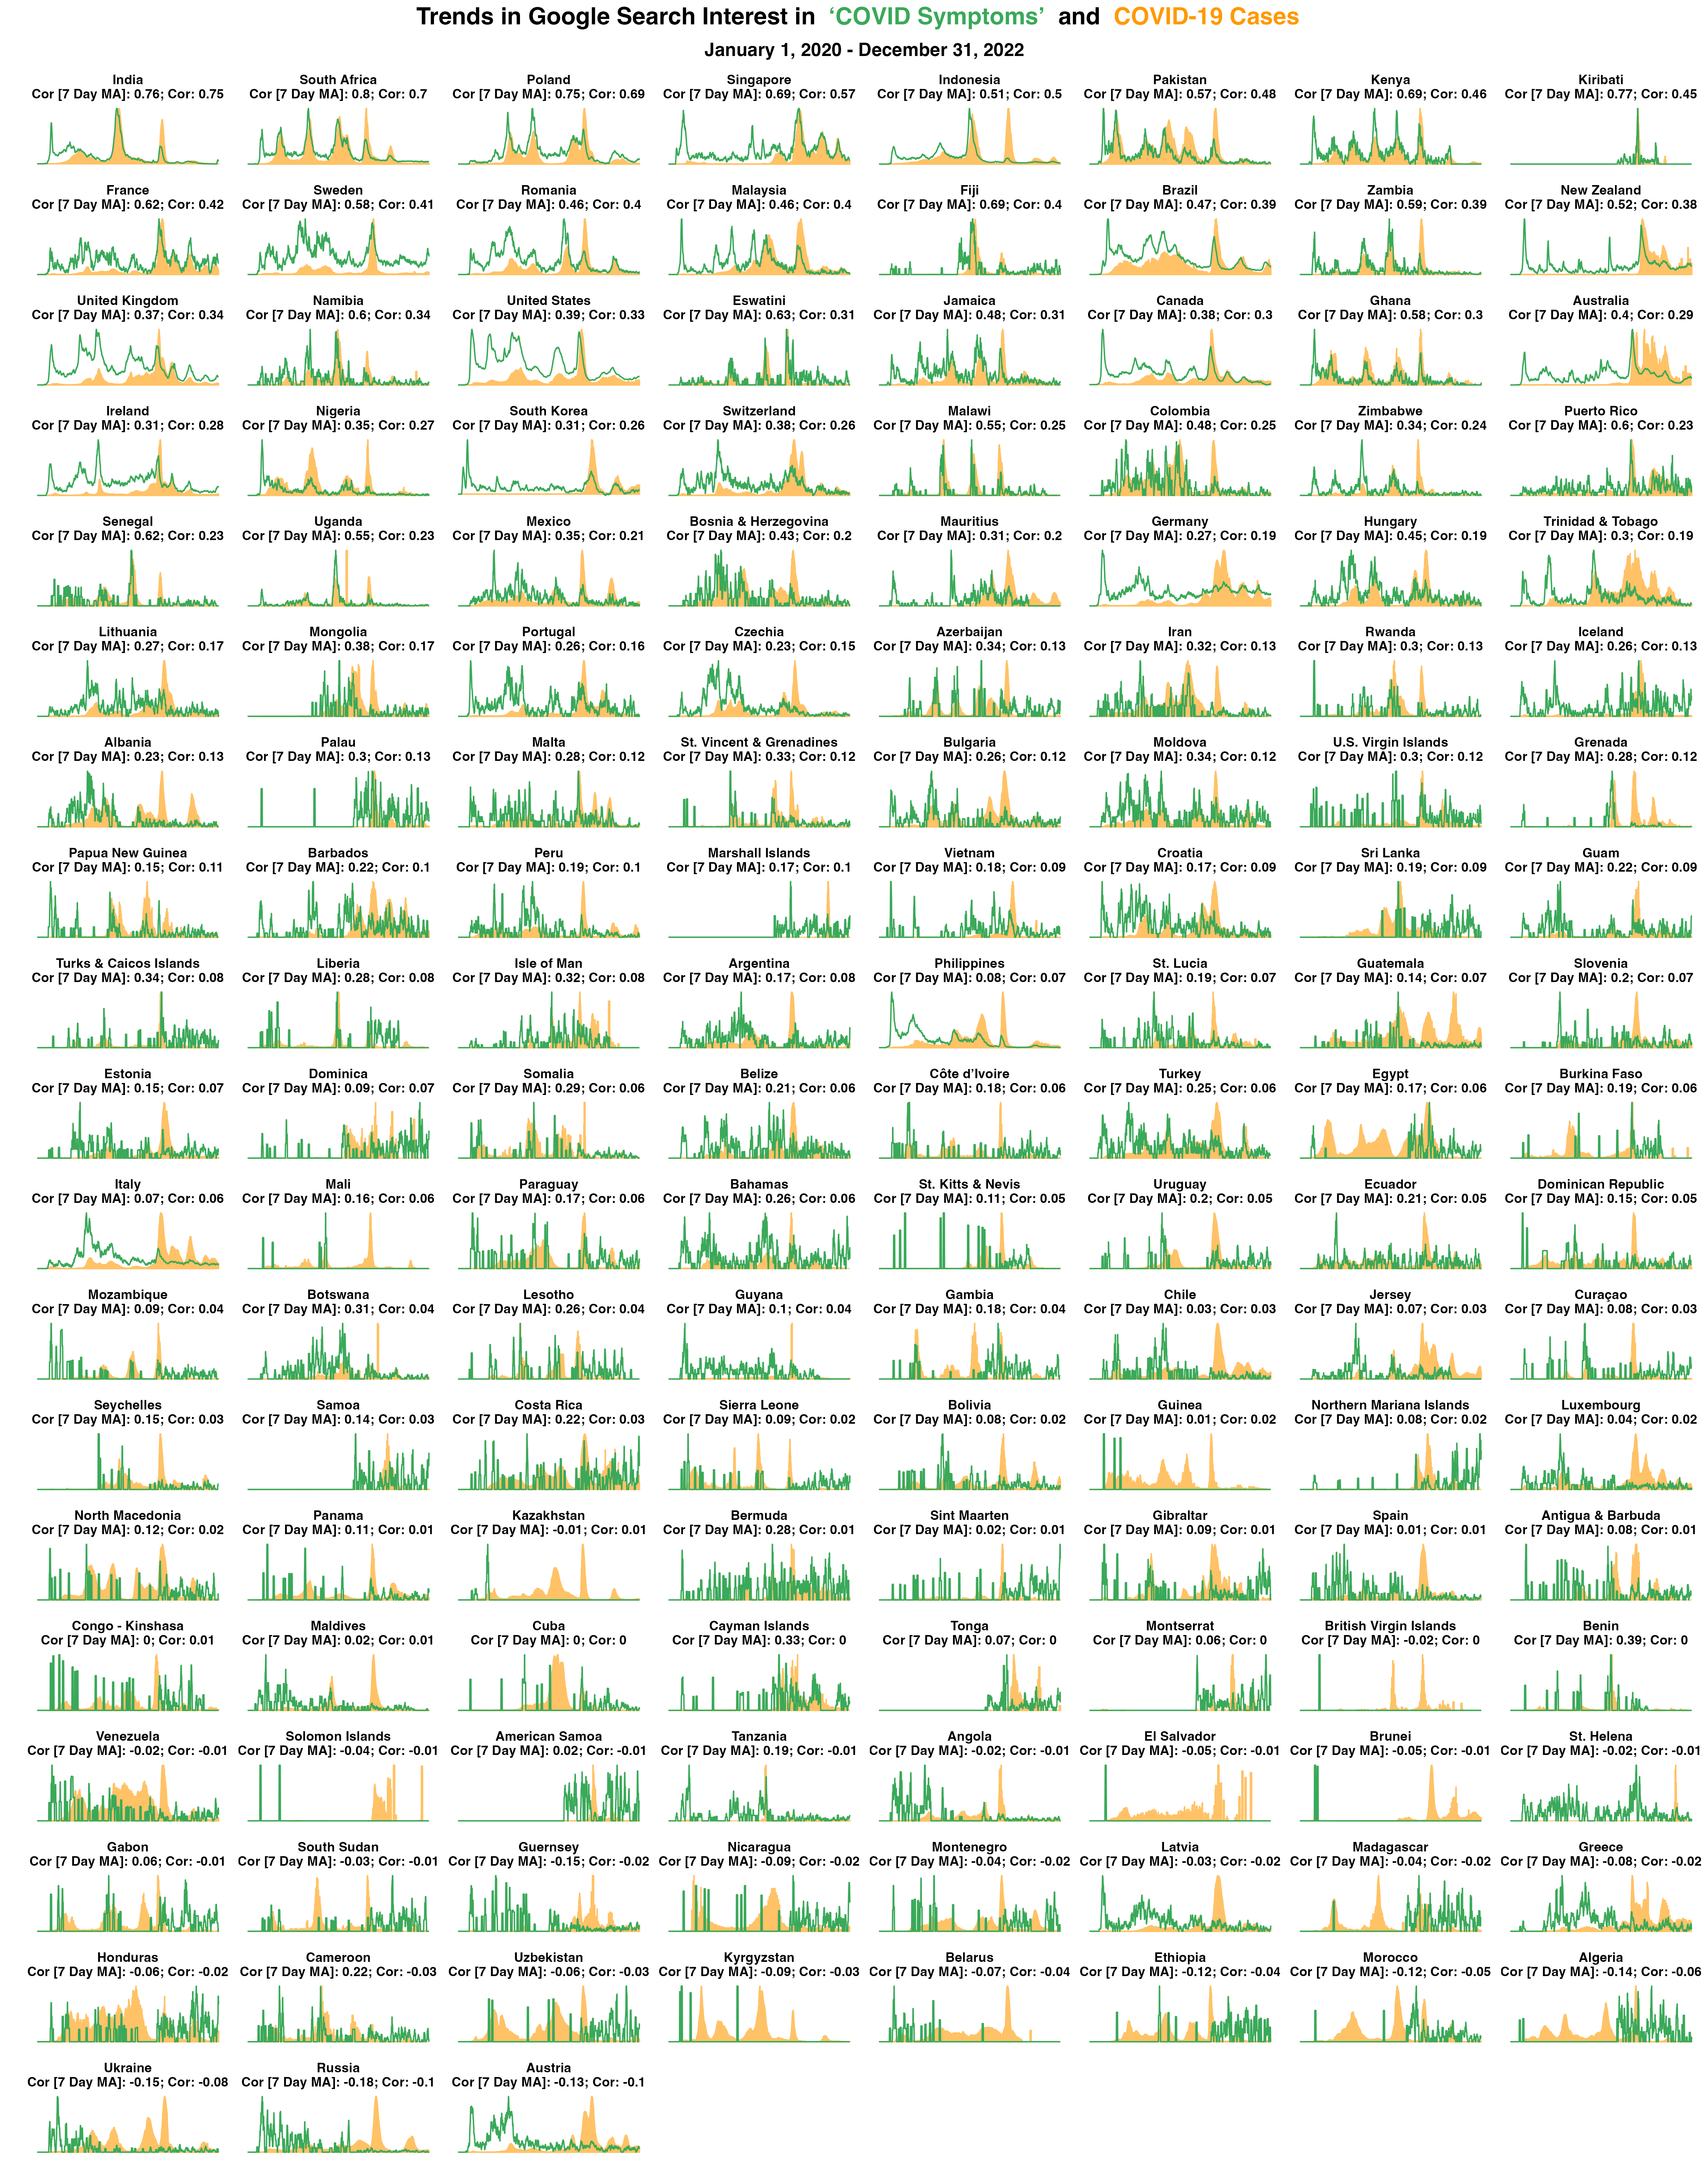
\includegraphics[width=1\textwidth]{figures/cases_vs_covid_symptoms_trends_allcountries.png}
    \caption{Trends between search interest in ``COVID Symptoms'' and COVID-19 cases for all countries with available data}
    \label{fig:cases_vs_covid_symptoms_trends_allcountries}
\end{figure}

% --------------------------
\newpage
\section{Trends in search interest for ``Coronavirus'' and COVID-19 cases for all countries with available data}
\label{si:coronavirus_covid_allcountries}

\begin{figure}[H]
    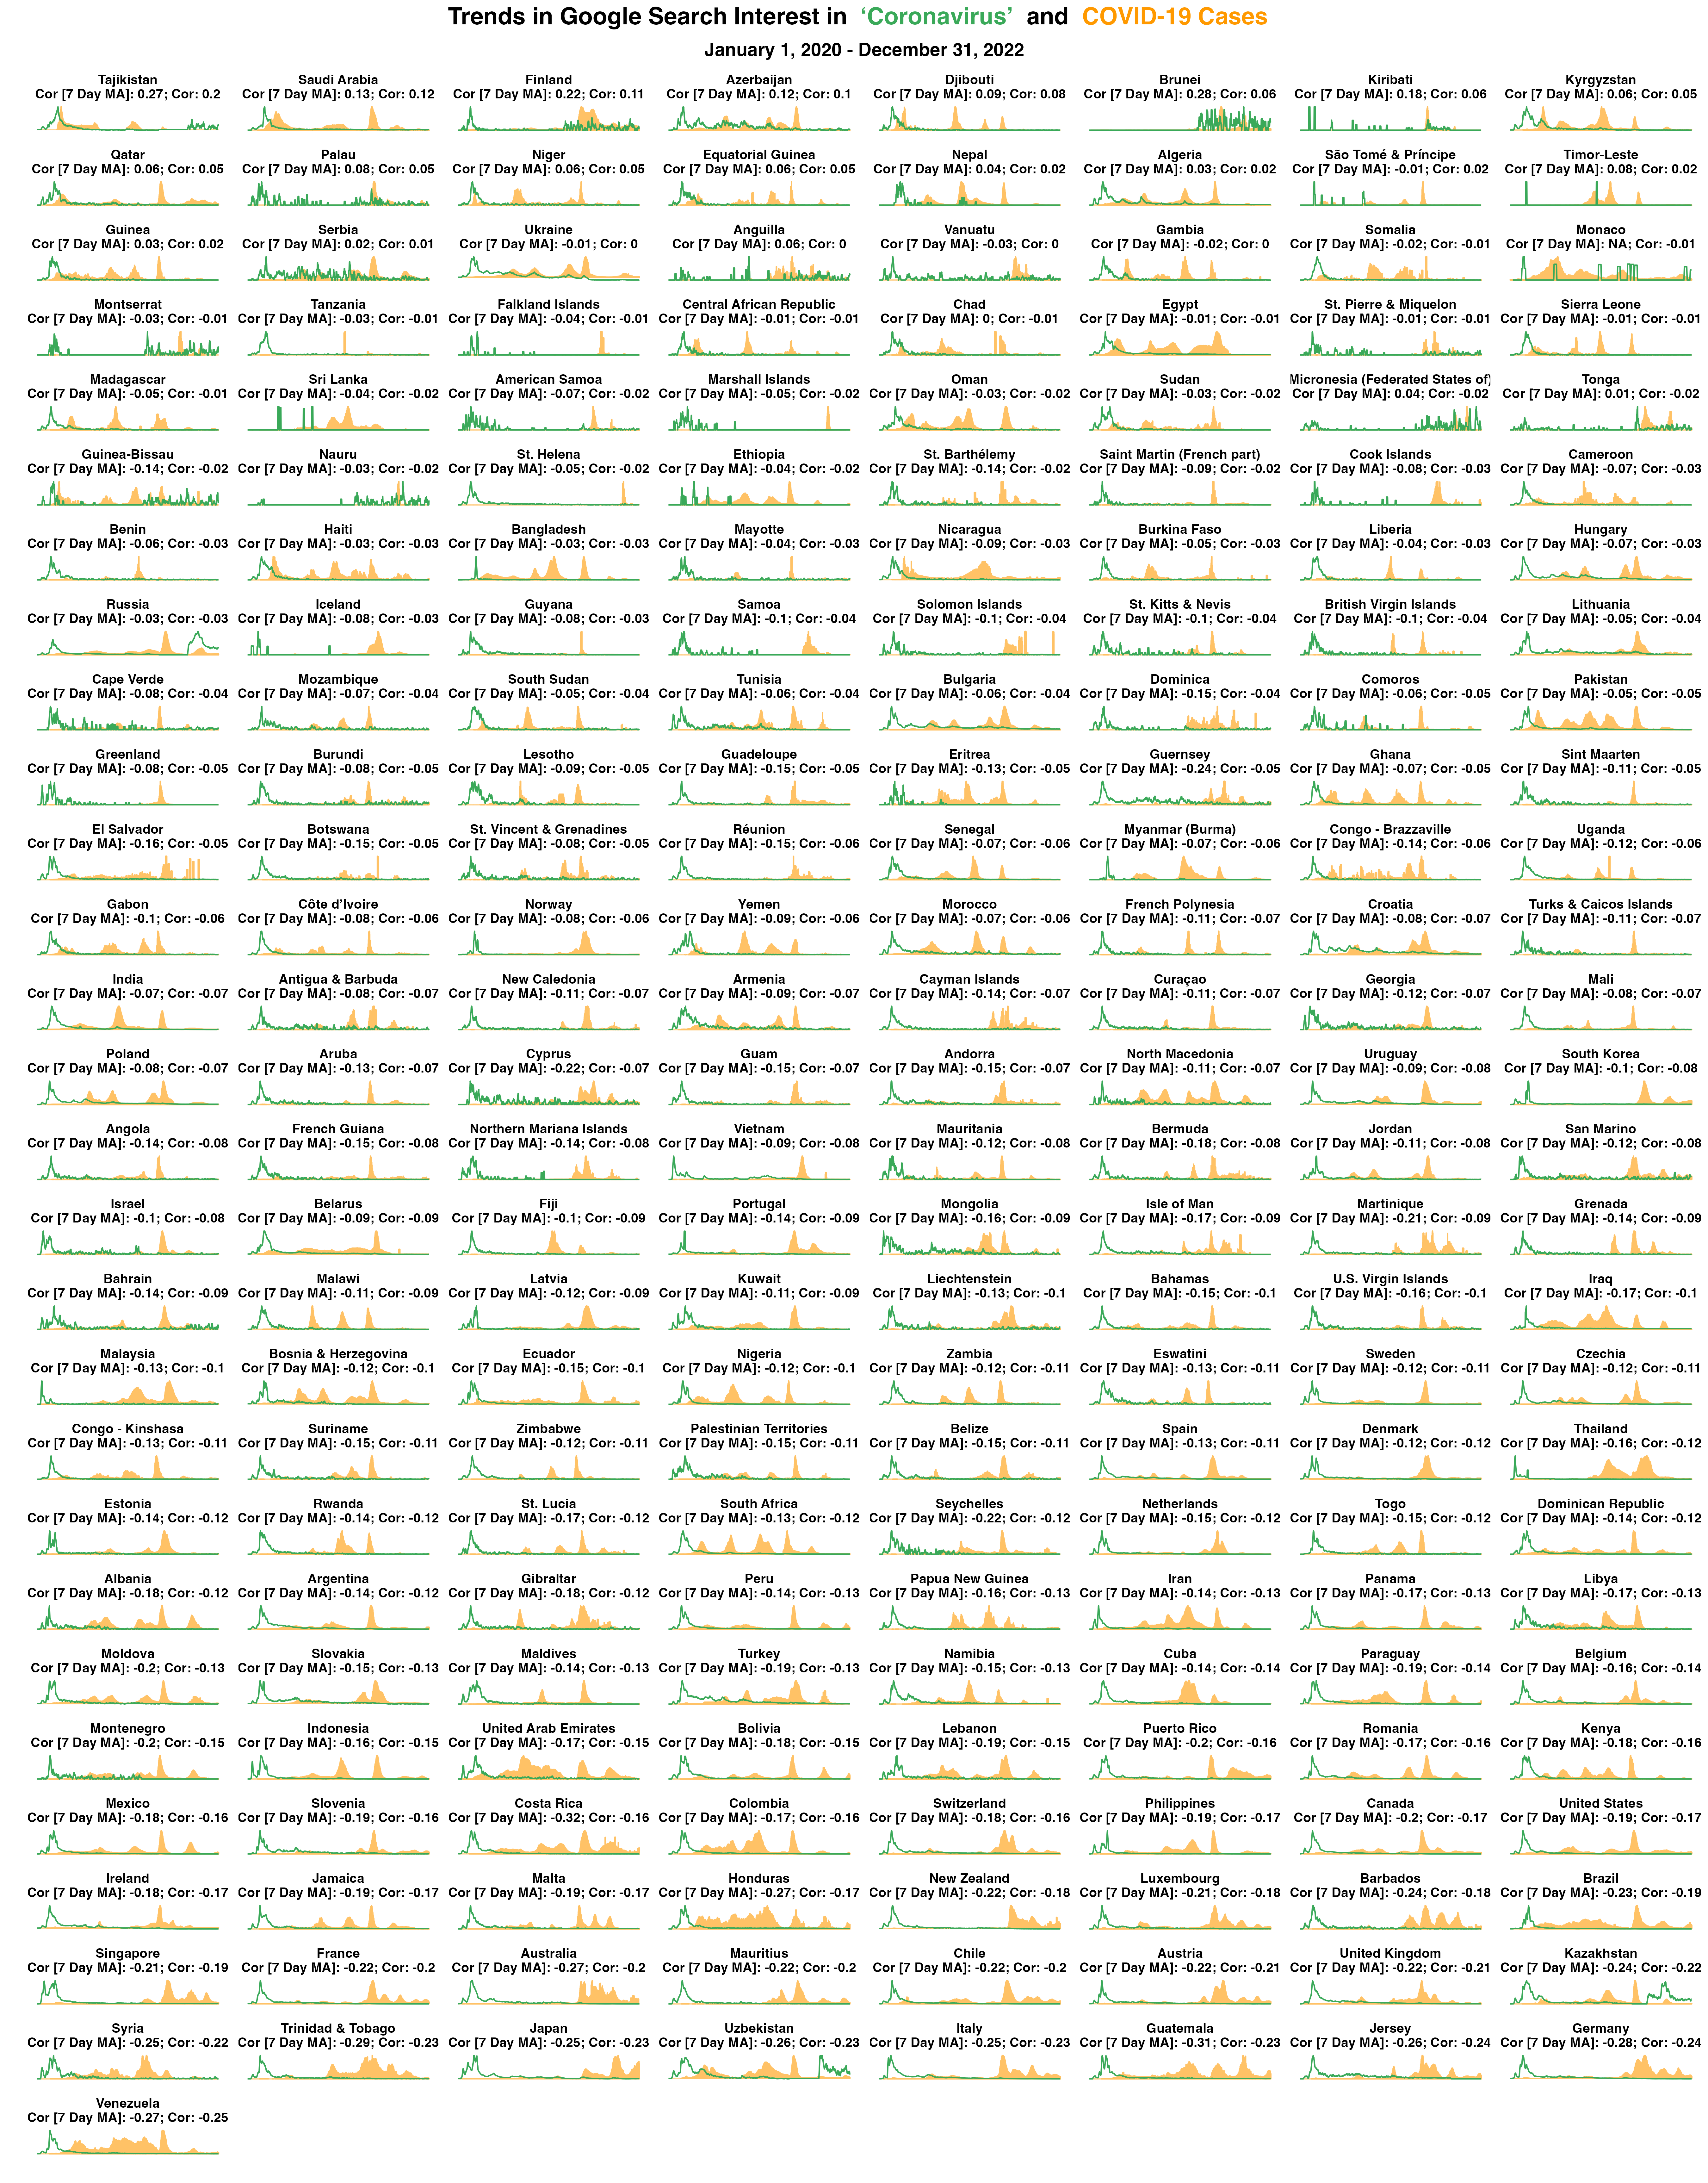
\includegraphics[width=1\textwidth]{figures/cases_vs_coronavirus_trends_allcountries.png}
    \caption{\textcolor{black}{Trends between search interest in ``COVID Symptoms'' and COVID-19 cases for all countries with available data}}
    \label{fig:cases_vs_coronavirus_trends_allcountries}
\end{figure}



% --------------------------
\newpage
\section{Correlation between search interest and reported COVID-19 cases by six months increments}
\label{si:boxplot_halfyears}

\begin{figure}[H]
    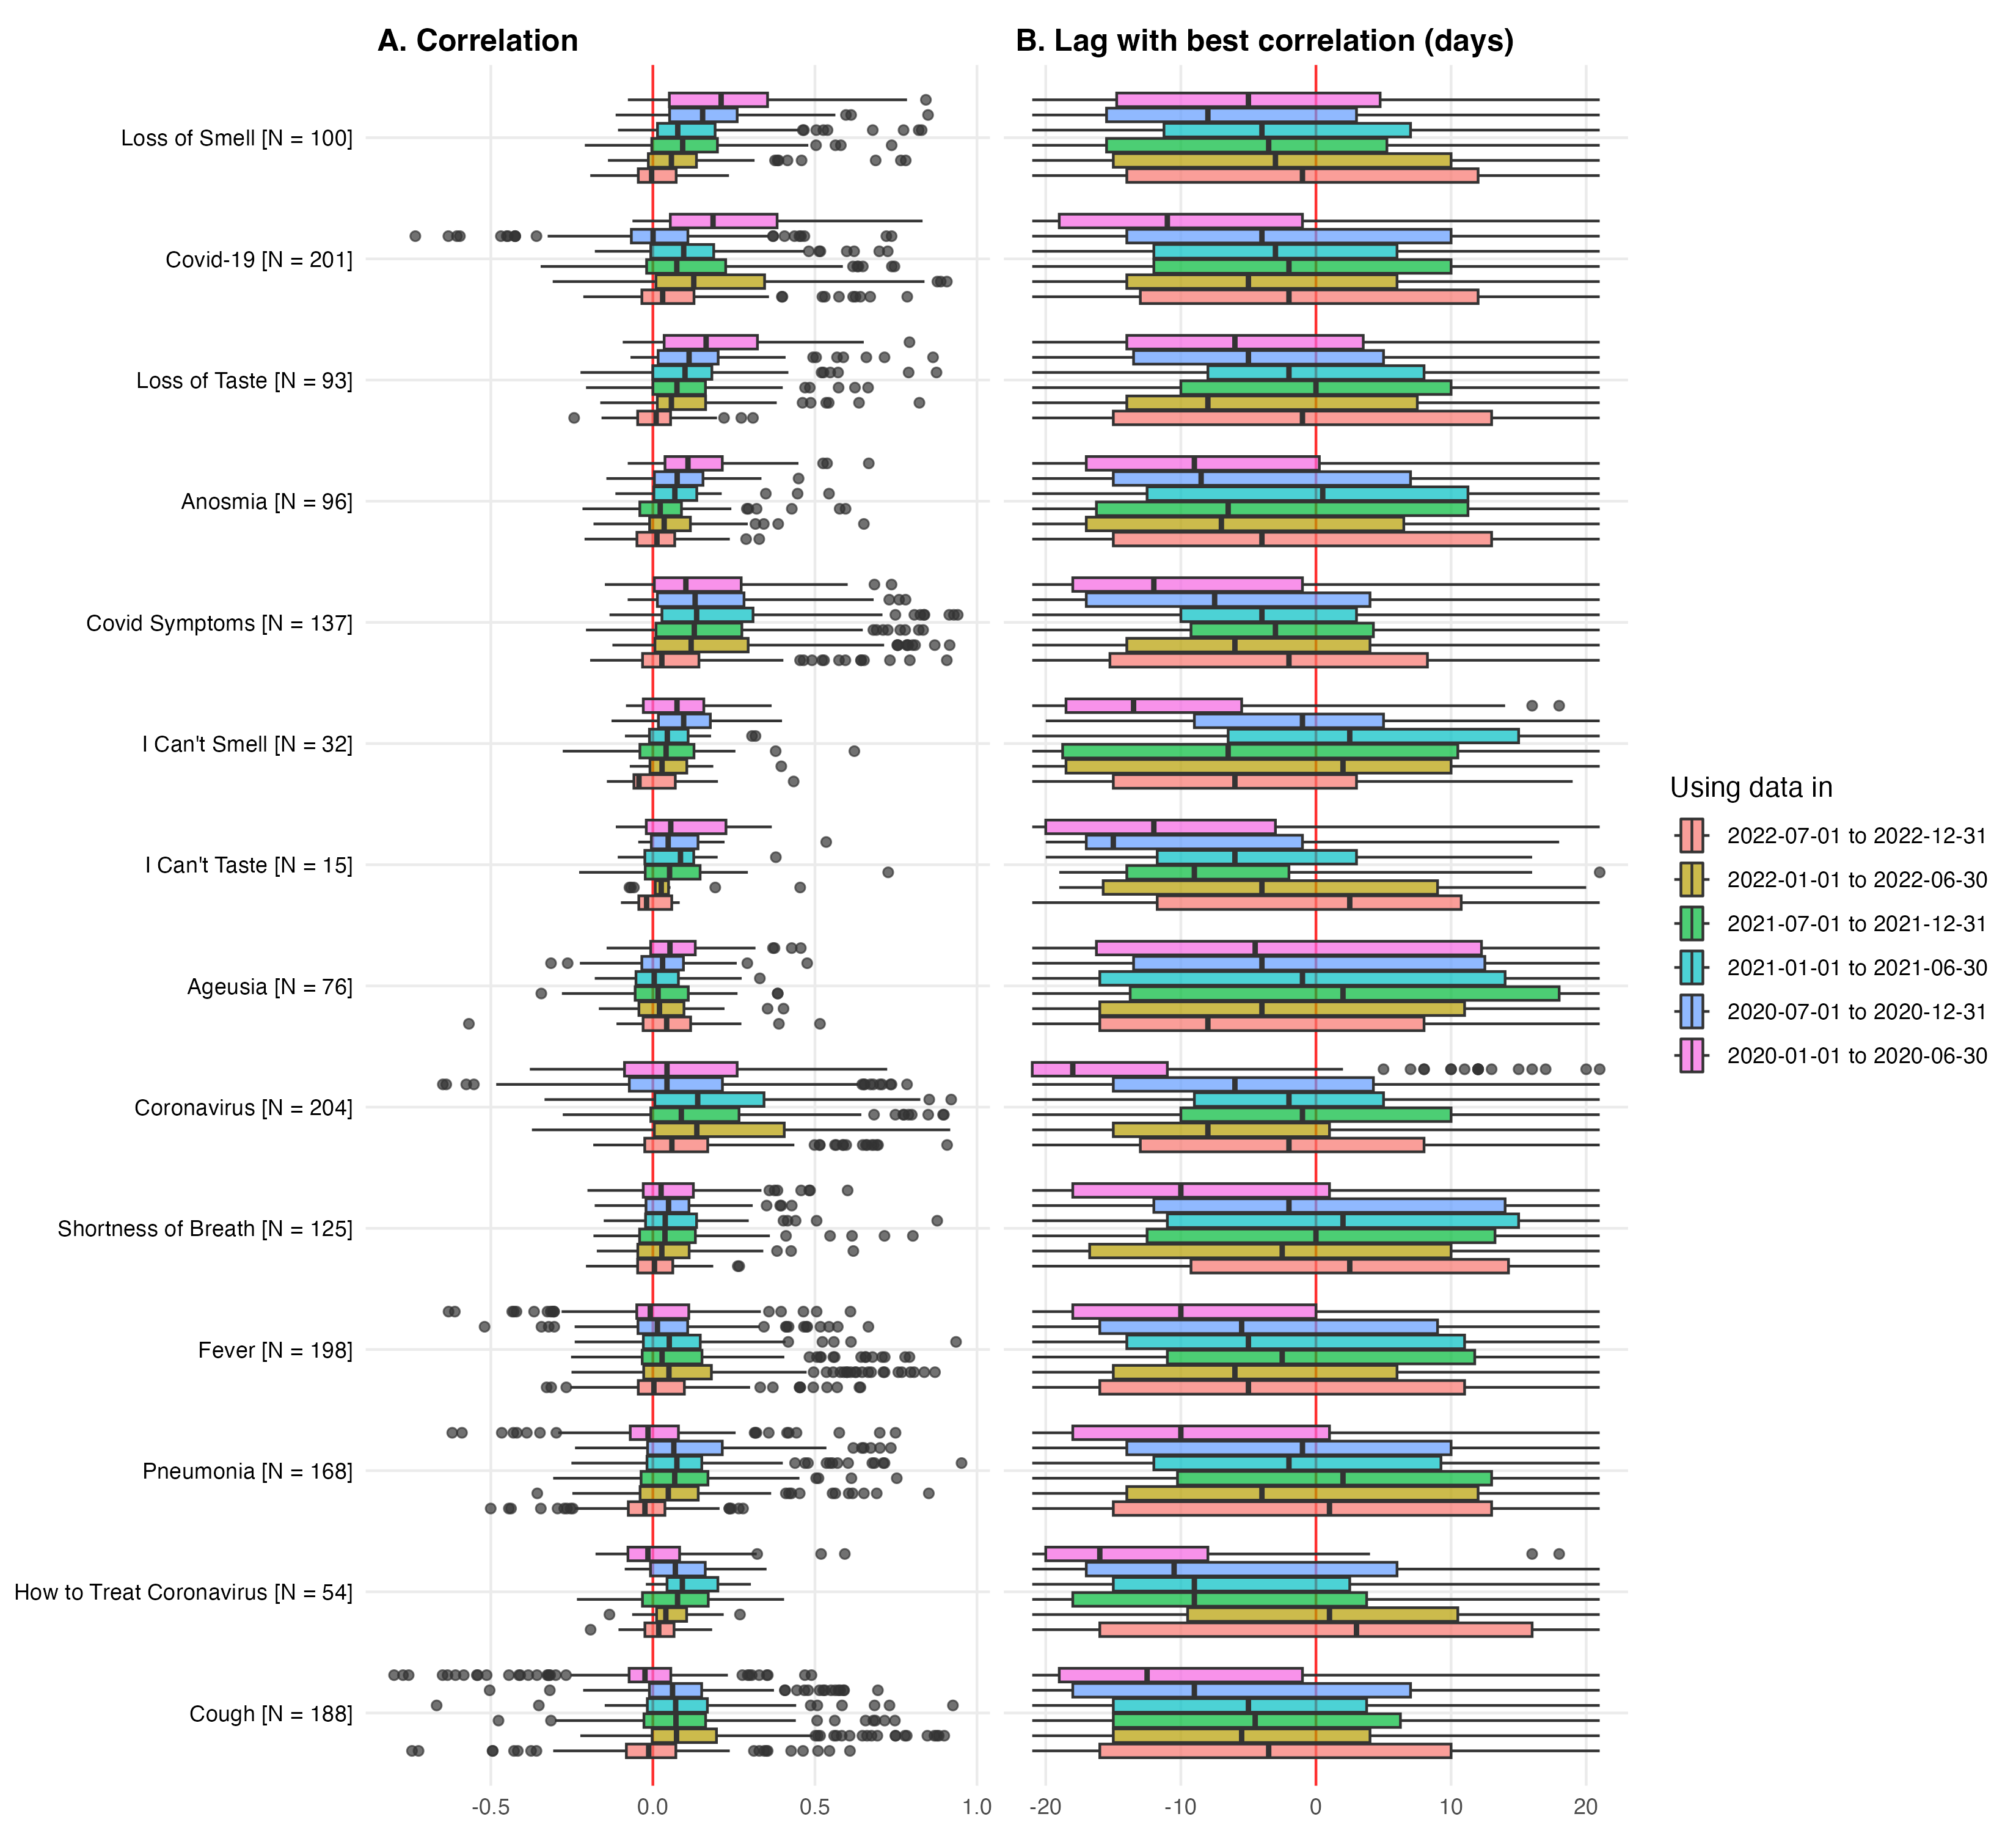
\includegraphics[width=1\textwidth]{figures/cor_halfyear_lag_fig.png}
    \caption{Search interest correlating with and anticipating COVID-19 cases. Panel A shows the correlation between search interest and COVID-19 cases. Panel B shows the lead/lad value of COVID-19 cases that produced the highest correlation with search interest. `N' indicates the number of countries with available data. The boxplots include: center line, median; box limits, upper and lower quartiles; whiskers, 1.5x interquartile range; points beyond whiskers, outliers.}
    \label{fig:cor_halfyear_lag_fig}
\end{figure}

% --------------------------
\newpage
\section{Explaining correlation between search interest and COVID-19 cases: additional results}
\label{si:lm_cor_searchinterest}

\newpage
\setlength{\tabcolsep}{4pt}
\begin{table}[H]
\centering
\caption{Explaining correlation between search interest in ``loss of taste'' and COVID-19 cases, using data from 2020 and 2021}

% Table created by stargazer v.5.2.3 by Marek Hlavac, Social Policy Institute. E-mail: marek.hlavac at gmail.com
% Date and time: Tue, Oct 03, 2023 - 06:36:10
% Requires LaTeX packages: dcolumn 
\begin{tabular}{@{\extracolsep{-15pt}}lD{.}{.}{-2} D{.}{.}{-2} D{.}{.}{-2} D{.}{.}{-2} D{.}{.}{-2} D{.}{.}{-2} D{.}{.}{-2} D{.}{.}{-2} } 
\\[-1.8ex]\hline 
\hline \\[-1.8ex] 
 & \multicolumn{8}{c}{\textit{Dependent variable:}} \\ 
\cline{2-9} 
\\[-1.8ex] & \multicolumn{8}{c}{Correlation} \\ 
\\[-1.8ex] & \multicolumn{1}{c}{(1)} & \multicolumn{1}{c}{(2)} & \multicolumn{1}{c}{(3)} & \multicolumn{1}{c}{(4)} & \multicolumn{1}{c}{(5)} & \multicolumn{1}{c}{(6)} & \multicolumn{1}{c}{(7)} & \multicolumn{1}{c}{(8)}\\ 
\hline \\[-1.8ex] 
 Total COVID-19 Cases, log & 0.03^{***} &  &  &  &  &  & 0.04^{***} & 0.04^{***} \\ 
  & (0.01) &  &  &  &  &  & (0.01) & (0.01) \\ 
  Per Pop. Using Internet &  & 0.0005 &  &  &  &  &  & -0.001 \\ 
  &  & (0.001) &  &  &  &  &  & (0.001) \\ 
  Mobile Cell Sub. per 100 &  &  & 0.0002 &  &  &  &  & 0.0002 \\ 
  &  &  & (0.001) &  &  &  &  & (0.001) \\ 
  GDP Per Cap, Log &  &  &  & 0.02 &  &  & -0.01 & -0.003 \\ 
  &  &  &  & (0.01) &  &  & (0.03) & (0.03) \\ 
  Low Income &  &  &  &  & -0.07 &  & 0.03 & 0.03 \\ 
  &  &  &  &  & (0.07) &  & (0.11) & (0.11) \\ 
  Lower Middle Income &  &  &  &  & -0.03 &  & 0.02 & 0.02 \\ 
  &  &  &  &  & (0.04) &  & (0.07) & (0.08) \\ 
  Upper Middle Income &  &  &  &  & -0.02 &  & 0.01 & 0.02 \\ 
  &  &  &  &  & (0.04) &  & (0.05) & (0.05) \\ 
  Europe and Central Asia &  &  &  &  &  & -0.02 & -0.02 & -0.02 \\ 
  &  &  &  &  &  & (0.05) & (0.05) & (0.05) \\ 
  Latin America and Caribbean &  &  &  &  &  & -0.07 & -0.04 & -0.04 \\ 
  &  &  &  &  &  & (0.05) & (0.05) & (0.05) \\ 
  Middle East and North Africa &  &  &  &  &  & -0.10^{*} & -0.07 & -0.06 \\ 
  &  &  &  &  &  & (0.05) & (0.05) & (0.06) \\ 
  North America &  &  &  &  &  & 0.37^{***} & 0.32^{***} & 0.32^{***} \\ 
  &  &  &  &  &  & (0.10) & (0.10) & (0.10) \\ 
  South Asia &  &  &  &  &  & 0.17^{**} & 0.15^{*} & 0.14^{*} \\ 
  &  &  &  &  &  & (0.09) & (0.08) & (0.09) \\ 
  Sub-Saharan Africa &  &  &  &  &  & -0.07 & -0.001 & -0.001 \\ 
  &  &  &  &  &  & (0.05) & (0.05) & (0.06) \\ 
  Constant & -0.35^{***} & 0.09^{*} & 0.10 & -0.03 & 0.14^{***} & 0.16^{***} & -0.27 & -0.35 \\ 
  & (0.09) & (0.05) & (0.06) & (0.10) & (0.03) & (0.04) & (0.28) & (0.30) \\ 
 \hline \\[-1.8ex] 
Observations & \multicolumn{1}{c}{105} & \multicolumn{1}{c}{100} & \multicolumn{1}{c}{103} & \multicolumn{1}{c}{102} & \multicolumn{1}{c}{102} & \multicolumn{1}{c}{105} & \multicolumn{1}{c}{102} & \multicolumn{1}{c}{100} \\ 
Adjusted R$^{2}$ & \multicolumn{1}{c}{0.20} & \multicolumn{1}{c}{-0.01} & \multicolumn{1}{c}{-0.01} & \multicolumn{1}{c}{0.01} & \multicolumn{1}{c}{-0.02} & \multicolumn{1}{c}{0.21} & \multicolumn{1}{c}{0.32} & \multicolumn{1}{c}{0.31} \\ 
\hline 
\hline \\[-1.8ex] 
\end{tabular} 
 \\
%\flushleft \addtabletext{$^{*}$p$<$0.1; $^{**}$p$<$0.05; $^{***}$p$<$0.01.}
\flushleft $^{*}$p$<$0.1; $^{**}$p$<$0.05; 
$^{***}$p$<$0.01\label{tab:cor_reg_table_loss_of_taste}
\label{tab:cor_reg_table_taste}
\end{table}

\setlength{\tabcolsep}{4pt}
\begin{table}[H]
\centering
\caption{Explaining the lead/lag value that produced the highest correlation between search interest in ``loss of taste'' and COVID-19 cases, using data from 2020 and 2021}

% Table created by stargazer v.5.2.3 by Marek Hlavac, Social Policy Institute. E-mail: marek.hlavac at gmail.com
% Date and time: Tue, Oct 03, 2023 - 06:36:11
% Requires LaTeX packages: dcolumn 
\begin{tabular}{@{\extracolsep{-15pt}}lD{.}{.}{-2} D{.}{.}{-2} D{.}{.}{-2} D{.}{.}{-2} D{.}{.}{-2} D{.}{.}{-2} D{.}{.}{-2} D{.}{.}{-2} } 
\\[-1.8ex]\hline 
\hline \\[-1.8ex] 
 & \multicolumn{8}{c}{\textit{Dependent variable:}} \\ 
\cline{2-9} 
\\[-1.8ex] & \multicolumn{8}{c}{Best Lag} \\ 
\\[-1.8ex] & \multicolumn{1}{c}{(1)} & \multicolumn{1}{c}{(2)} & \multicolumn{1}{c}{(3)} & \multicolumn{1}{c}{(4)} & \multicolumn{1}{c}{(5)} & \multicolumn{1}{c}{(6)} & \multicolumn{1}{c}{(7)} & \multicolumn{1}{c}{(8)}\\ 
\hline \\[-1.8ex] 
 Total COVID-19 Cases, log & -0.79 &  &  &  &  &  & -1.09^{*} & -1.20^{*} \\ 
  & (0.51) &  &  &  &  &  & (0.64) & (0.67) \\ 
  Per Pop. Using Internet &  & -0.03 &  &  &  &  &  & 0.04 \\ 
  &  & (0.05) &  &  &  &  &  & (0.11) \\ 
  Mobile Cell Sub. per 100 &  &  & 0.01 &  &  &  &  & 0.002 \\ 
  &  &  & (0.04) &  &  &  &  & (0.04) \\ 
  GDP Per Cap, Log &  &  &  & -0.20 &  &  & 1.74 & 0.92 \\ 
  &  &  &  & (0.81) &  &  & (2.10) & (2.51) \\ 
  Low Income &  &  &  &  & 7.13 &  & 4.01 & 4.04 \\ 
  &  &  &  &  & (4.49) &  & (8.36) & (8.66) \\ 
  Lower Middle Income &  &  &  &  & -1.71 &  & -1.19 & -1.21 \\ 
  &  &  &  &  & (2.54) &  & (5.83) & (5.93) \\ 
  Upper Middle Income &  &  &  &  & 3.08 &  & 5.53 & 4.96 \\ 
  &  &  &  &  & (2.50) &  & (3.87) & (4.00) \\ 
  Europe and Central Asia &  &  &  &  &  & -2.10 & -3.59 & -3.38 \\ 
  &  &  &  &  &  & (3.48) & (3.55) & (3.68) \\ 
  Latin America and Caribbean &  &  &  &  &  & -7.52^{**} & -9.75^{**} & -9.76^{**} \\ 
  &  &  &  &  &  & (3.68) & (3.81) & (3.90) \\ 
  Middle East and North Africa &  &  &  &  &  & -7.22^{*} & -7.79^{*} & -8.50^{*} \\ 
  &  &  &  &  &  & (4.08) & (4.06) & (4.32) \\ 
  North America &  &  &  &  &  & -1.30 & -0.98 & -0.44 \\ 
  &  &  &  &  &  & (7.52) & (7.55) & (7.89) \\ 
  South Asia &  &  &  &  &  & -5.63 & -3.84 & -3.47 \\ 
  &  &  &  &  &  & (6.39) & (6.41) & (6.68) \\ 
  Sub-Saharan Africa &  &  &  &  &  & 3.44 & 2.45 & 2.26 \\ 
  &  &  &  &  &  & (3.79) & (4.28) & (4.55) \\ 
  Constant & 4.40 & -4.61 & -8.18^{*} & -4.61 & -7.29^{***} & -3.70 & -4.58 & 1.51 \\ 
  & (7.08) & (3.17) & (4.24) & (7.32) & (1.74) & (3.07) & (22.22) & (23.44) \\ 
 \hline \\[-1.8ex] 
Observations & \multicolumn{1}{c}{105} & \multicolumn{1}{c}{100} & \multicolumn{1}{c}{103} & \multicolumn{1}{c}{102} & \multicolumn{1}{c}{102} & \multicolumn{1}{c}{105} & \multicolumn{1}{c}{102} & \multicolumn{1}{c}{100} \\ 
Adjusted R$^{2}$ & \multicolumn{1}{c}{0.01} & \multicolumn{1}{c}{-0.01} & \multicolumn{1}{c}{-0.01} & \multicolumn{1}{c}{-0.01} & \multicolumn{1}{c}{0.03} & \multicolumn{1}{c}{0.10} & \multicolumn{1}{c}{0.15} & \multicolumn{1}{c}{0.13} \\ 
\hline 
\hline \\[-1.8ex] 
\end{tabular} 
 \\
%\flushleft \addtabletext{$^{*}$p$<$0.1; $^{**}$p$<$0.05; $^{***}$p$<$0.01.}
\flushleft $^{*}$p$<$0.1; $^{**}$p$<$0.05; $^{***}$p$<$0.01
\label{tab:lag_reg_table_loss_of_taste}
\end{table}

%%%% COVID Symptoms
\setlength{\tabcolsep}{4pt}
\begin{table}[H]
\centering
\caption{Explaining correlation between search interest in ``COVID symptoms'' and COVID-19 cases, using data from 2020 and 2021}

% Table created by stargazer v.5.2.3 by Marek Hlavac, Social Policy Institute. E-mail: marek.hlavac at gmail.com
% Date and time: Fri, Oct 13, 2023 - 09:00:10
% Requires LaTeX packages: dcolumn 
\begin{tabular}{@{\extracolsep{-15pt}}lD{.}{.}{-2} D{.}{.}{-2} D{.}{.}{-2} D{.}{.}{-2} D{.}{.}{-2} D{.}{.}{-2} D{.}{.}{-2} D{.}{.}{-2} } 
\\[-1.8ex]\hline 
\hline \\[-1.8ex] 
 & \multicolumn{8}{c}{\textit{Dependent variable:}} \\ 
\cline{2-9} 
\\[-1.8ex] & \multicolumn{8}{c}{Correlation} \\ 
\\[-1.8ex] & \multicolumn{1}{c}{(1)} & \multicolumn{1}{c}{(2)} & \multicolumn{1}{c}{(3)} & \multicolumn{1}{c}{(4)} & \multicolumn{1}{c}{(5)} & \multicolumn{1}{c}{(6)} & \multicolumn{1}{c}{(7)} & \multicolumn{1}{c}{(8)}\\ 
\hline \\[-1.8ex] 
 Total COVID-19 Cases, log & 0.03^{***} &  &  &  &  &  & 0.03^{***} & 0.03^{***} \\ 
  & (0.01) &  &  &  &  &  & (0.01) & (0.01) \\ 
  Per Pop. Using Internet &  & 0.001 &  &  &  &  &  & -0.004^{*} \\ 
  &  & (0.001) &  &  &  &  &  & (0.002) \\ 
  Mobile Cell Sub. per 100 &  &  & 0.0005 &  &  &  &  & -0.0003 \\ 
  &  &  & (0.0005) &  &  &  &  & (0.001) \\ 
  GDP Per Cap, Log &  &  &  & 0.03^{**} &  &  & -0.001 & 0.04 \\ 
  &  &  &  & (0.01) &  &  & (0.03) & (0.04) \\ 
  Low Income &  &  &  &  & -0.10^{*} &  & -0.13 & -0.19 \\ 
  &  &  &  &  & (0.05) &  & (0.13) & (0.15) \\ 
  Lower Middle Income &  &  &  &  & -0.07^{*} &  & -0.10 & -0.13 \\ 
  &  &  &  &  & (0.04) &  & (0.09) & (0.10) \\ 
  Upper Middle Income &  &  &  &  & -0.05 &  & -0.05 & -0.04 \\ 
  &  &  &  &  & (0.04) &  & (0.06) & (0.06) \\ 
  Europe and Central Asia &  &  &  &  &  & 0.04 & -0.04 & -0.03 \\ 
  &  &  &  &  &  & (0.05) & (0.05) & (0.06) \\ 
  Latin America and Caribbean &  &  &  &  &  & -0.02 & -0.01 & -0.03 \\ 
  &  &  &  &  &  & (0.05) & (0.05) & (0.06) \\ 
  Middle East and North Africa &  &  &  &  &  & -0.11 & -0.11 & -0.06 \\ 
  &  &  &  &  &  & (0.09) & (0.09) & (0.09) \\ 
  North America &  &  &  &  &  & 0.20^{*} & 0.08 & 0.13 \\ 
  &  &  &  &  &  & (0.11) & (0.11) & (0.14) \\ 
  South Asia &  &  &  &  &  & 0.21^{**} & 0.18^{*} & 0.15 \\ 
  &  &  &  &  &  & (0.10) & (0.09) & (0.10) \\ 
  Sub-Saharan Africa &  &  &  &  &  & -0.005 & 0.09 & 0.05 \\ 
  &  &  &  &  &  & (0.05) & (0.06) & (0.07) \\ 
  Constant & -0.26^{***} & 0.11^{**} & 0.10^{*} & -0.08 & 0.20^{***} & 0.14^{***} & -0.23 & -0.31 \\ 
  & (0.07) & (0.05) & (0.06) & (0.10) & (0.03) & (0.04) & (0.35) & (0.40) \\ 
 \hline \\[-1.8ex] 
Observations & \multicolumn{1}{c}{145} & \multicolumn{1}{c}{125} & \multicolumn{1}{c}{135} & \multicolumn{1}{c}{137} & \multicolumn{1}{c}{140} & \multicolumn{1}{c}{145} & \multicolumn{1}{c}{137} & \multicolumn{1}{c}{124} \\ 
Adjusted R$^{2}$ & \multicolumn{1}{c}{0.18} & \multicolumn{1}{c}{0.01} & \multicolumn{1}{c}{0.0003} & \multicolumn{1}{c}{0.03} & \multicolumn{1}{c}{0.02} & \multicolumn{1}{c}{0.04} & \multicolumn{1}{c}{0.21} & \multicolumn{1}{c}{0.20} \\ 
\hline 
\hline \\[-1.8ex] 
\end{tabular} 
 \\
%\flushleft \addtabletext{$^{*}$p$<$0.1; $^{**}$p$<$0.05; $^{***}$p$<$0.01.}
\flushleft $^{*}$p$<$0.1; $^{**}$p$<$0.05; $^{***}$p$<$0.01
\label{tab:cor_reg_table_covidsymptoms}
\end{table}

\setlength{\tabcolsep}{4pt}
\begin{table}[H]
\centering
\caption{Explaining the lead/lag value that produced the highest correlation between search interest in ``COVID symptoms'' and COVID-19 cases, using data from 2020 and 2021}

% Table created by stargazer v.5.2.3 by Marek Hlavac, Social Policy Institute. E-mail: marek.hlavac at gmail.com
% Date and time: Fri, Oct 13, 2023 - 09:00:11
% Requires LaTeX packages: dcolumn 
\begin{tabular}{@{\extracolsep{-15pt}}lD{.}{.}{-2} D{.}{.}{-2} D{.}{.}{-2} D{.}{.}{-2} D{.}{.}{-2} D{.}{.}{-2} D{.}{.}{-2} D{.}{.}{-2} } 
\\[-1.8ex]\hline 
\hline \\[-1.8ex] 
 & \multicolumn{8}{c}{\textit{Dependent variable:}} \\ 
\cline{2-9} 
\\[-1.8ex] & \multicolumn{8}{c}{Best Lag} \\ 
\\[-1.8ex] & \multicolumn{1}{c}{(1)} & \multicolumn{1}{c}{(2)} & \multicolumn{1}{c}{(3)} & \multicolumn{1}{c}{(4)} & \multicolumn{1}{c}{(5)} & \multicolumn{1}{c}{(6)} & \multicolumn{1}{c}{(7)} & \multicolumn{1}{c}{(8)}\\ 
\hline \\[-1.8ex] 
 Total COVID-19 Cases, log & -0.44 &  &  &  &  &  & -0.37 & -0.10 \\ 
  & (0.31) &  &  &  &  &  & (0.38) & (0.45) \\ 
  Per Pop. Using Internet &  & -0.02 &  &  &  &  &  & -0.02 \\ 
  &  & (0.03) &  &  &  &  &  & (0.10) \\ 
  Mobile Cell Sub. per 100 &  &  & 0.01 &  &  &  &  & -0.02 \\ 
  &  &  & (0.02) &  &  &  &  & (0.03) \\ 
  GDP Per Cap, Log &  &  &  & 0.41 &  &  & 2.59 & 1.05 \\ 
  &  &  &  & (0.57) &  &  & (1.79) & (2.22) \\ 
  Low Income &  &  &  &  & -0.27 &  & 1.98 & -3.82 \\ 
  &  &  &  &  & (2.61) &  & (7.11) & (7.64) \\ 
  Lower Middle Income &  &  &  &  & -1.31 &  & 1.71 & -2.68 \\ 
  &  &  &  &  & (2.04) &  & (5.01) & (5.37) \\ 
  Upper Middle Income &  &  &  &  & -2.40 &  & 0.59 & -1.52 \\ 
  &  &  &  &  & (1.92) &  & (3.10) & (3.28) \\ 
  Europe and Central Asia &  &  &  &  &  & -0.35 & -0.24 & -0.76 \\ 
  &  &  &  &  &  & (2.47) & (2.74) & (2.97) \\ 
  Latin America and Caribbean &  &  &  &  &  & -0.19 & -0.29 & -2.08 \\ 
  &  &  &  &  &  & (2.48) & (2.63) & (3.00) \\ 
  Middle East and North Africa &  &  &  &  &  & 5.70 & 6.83 & 7.27 \\ 
  &  &  &  &  &  & (4.51) & (4.65) & (4.77) \\ 
  North America &  &  &  &  &  & 4.63 & 1.30 & 2.27 \\ 
  &  &  &  &  &  & (5.59) & (5.89) & (7.05) \\ 
  South Asia &  &  &  &  &  & -0.70 & 2.15 & 1.24 \\ 
  &  &  &  &  &  & (4.94) & (5.11) & (5.20) \\ 
  Sub-Saharan Africa &  &  &  &  &  & 3.09 & 6.87^{**} & 6.04^{*} \\ 
  &  &  &  &  &  & (2.54) & (3.19) & (3.56) \\ 
  Constant & -0.83 & -5.35^{**} & -7.37^{***} & -10.07^{*} & -5.36^{***} & -7.30^{***} & -27.34 & -10.99 \\ 
  & (3.99) & (2.07) & (2.66) & (5.15) & (1.29) & (2.02) & (19.08) & (20.53) \\ 
 \hline \\[-1.8ex] 
Observations & \multicolumn{1}{c}{145} & \multicolumn{1}{c}{125} & \multicolumn{1}{c}{135} & \multicolumn{1}{c}{137} & \multicolumn{1}{c}{140} & \multicolumn{1}{c}{145} & \multicolumn{1}{c}{137} & \multicolumn{1}{c}{124} \\ 
Adjusted R$^{2}$ & \multicolumn{1}{c}{0.01} & \multicolumn{1}{c}{-0.004} & \multicolumn{1}{c}{-0.01} & \multicolumn{1}{c}{-0.004} & \multicolumn{1}{c}{-0.01} & \multicolumn{1}{c}{-0.003} & \multicolumn{1}{c}{0.01} & \multicolumn{1}{c}{-0.0005} \\ 
\hline 
\hline \\[-1.8ex] 
\end{tabular} 
 \\
%\flushleft \addtabletext{$^{*}$p$<$0.1; $^{**}$p$<$0.05; $^{***}$p$<$0.01.}
\flushleft $^{*}$p$<$0.1; $^{**}$p$<$0.05; $^{***}$p$<$0.01\label{tab:lm_lag_daily_covid_symptoms}
\end{table}

%% Figures
\begin{figure}[H]
    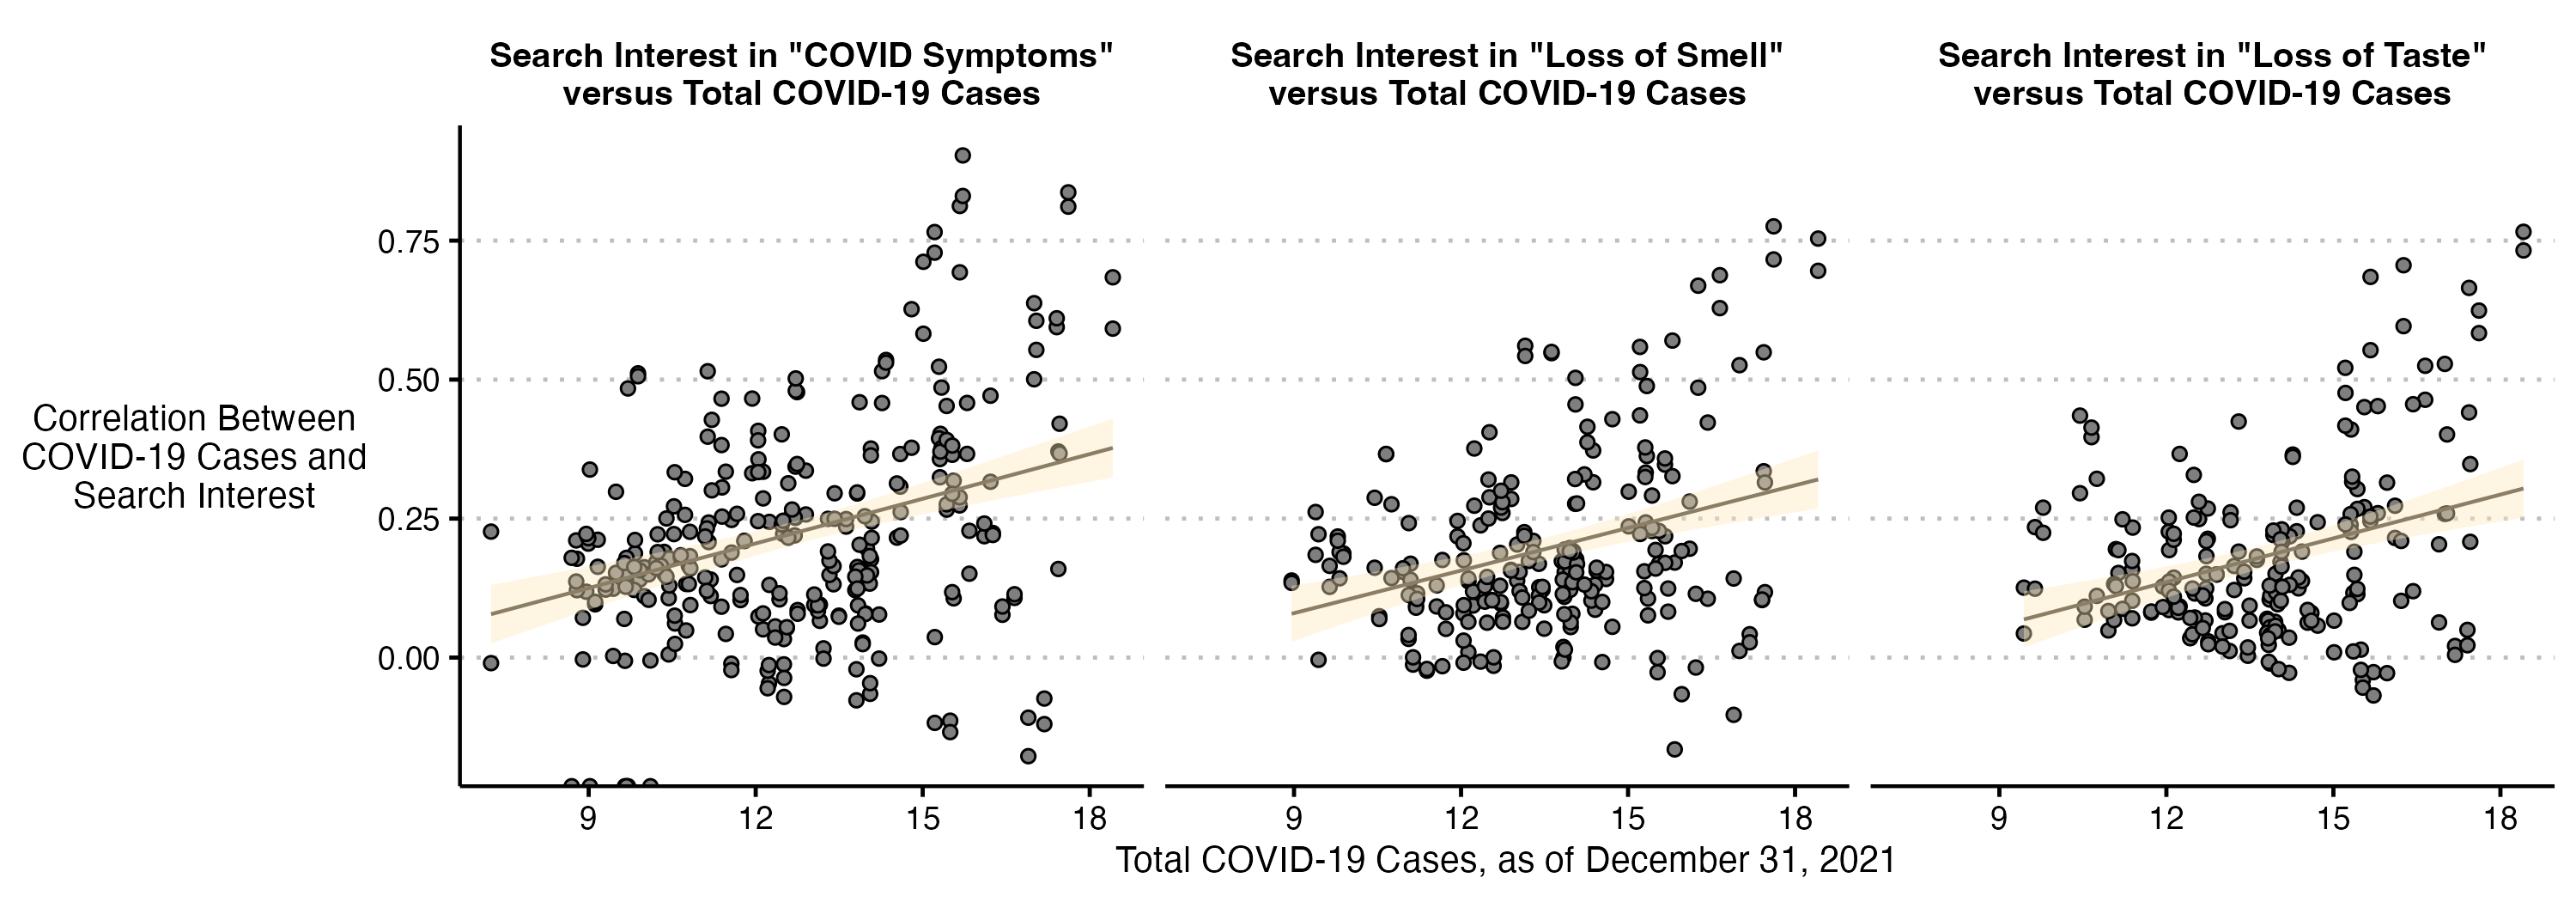
\includegraphics[width=1\textwidth]{figures/cor_casestotal_scatter.png}
    \caption{Scatterplots showing association between (1) correlation of search interest and COVID-19 cases and (2) total COVID-19 cases as of December 31, 2021, for search interest in ``COVID Symptoms'', ``Loss of Smell'', and ``Loss of Taste.''}
    \label{fig:cor_casestotal_scatter}
\end{figure}

\begin{figure}[H]
    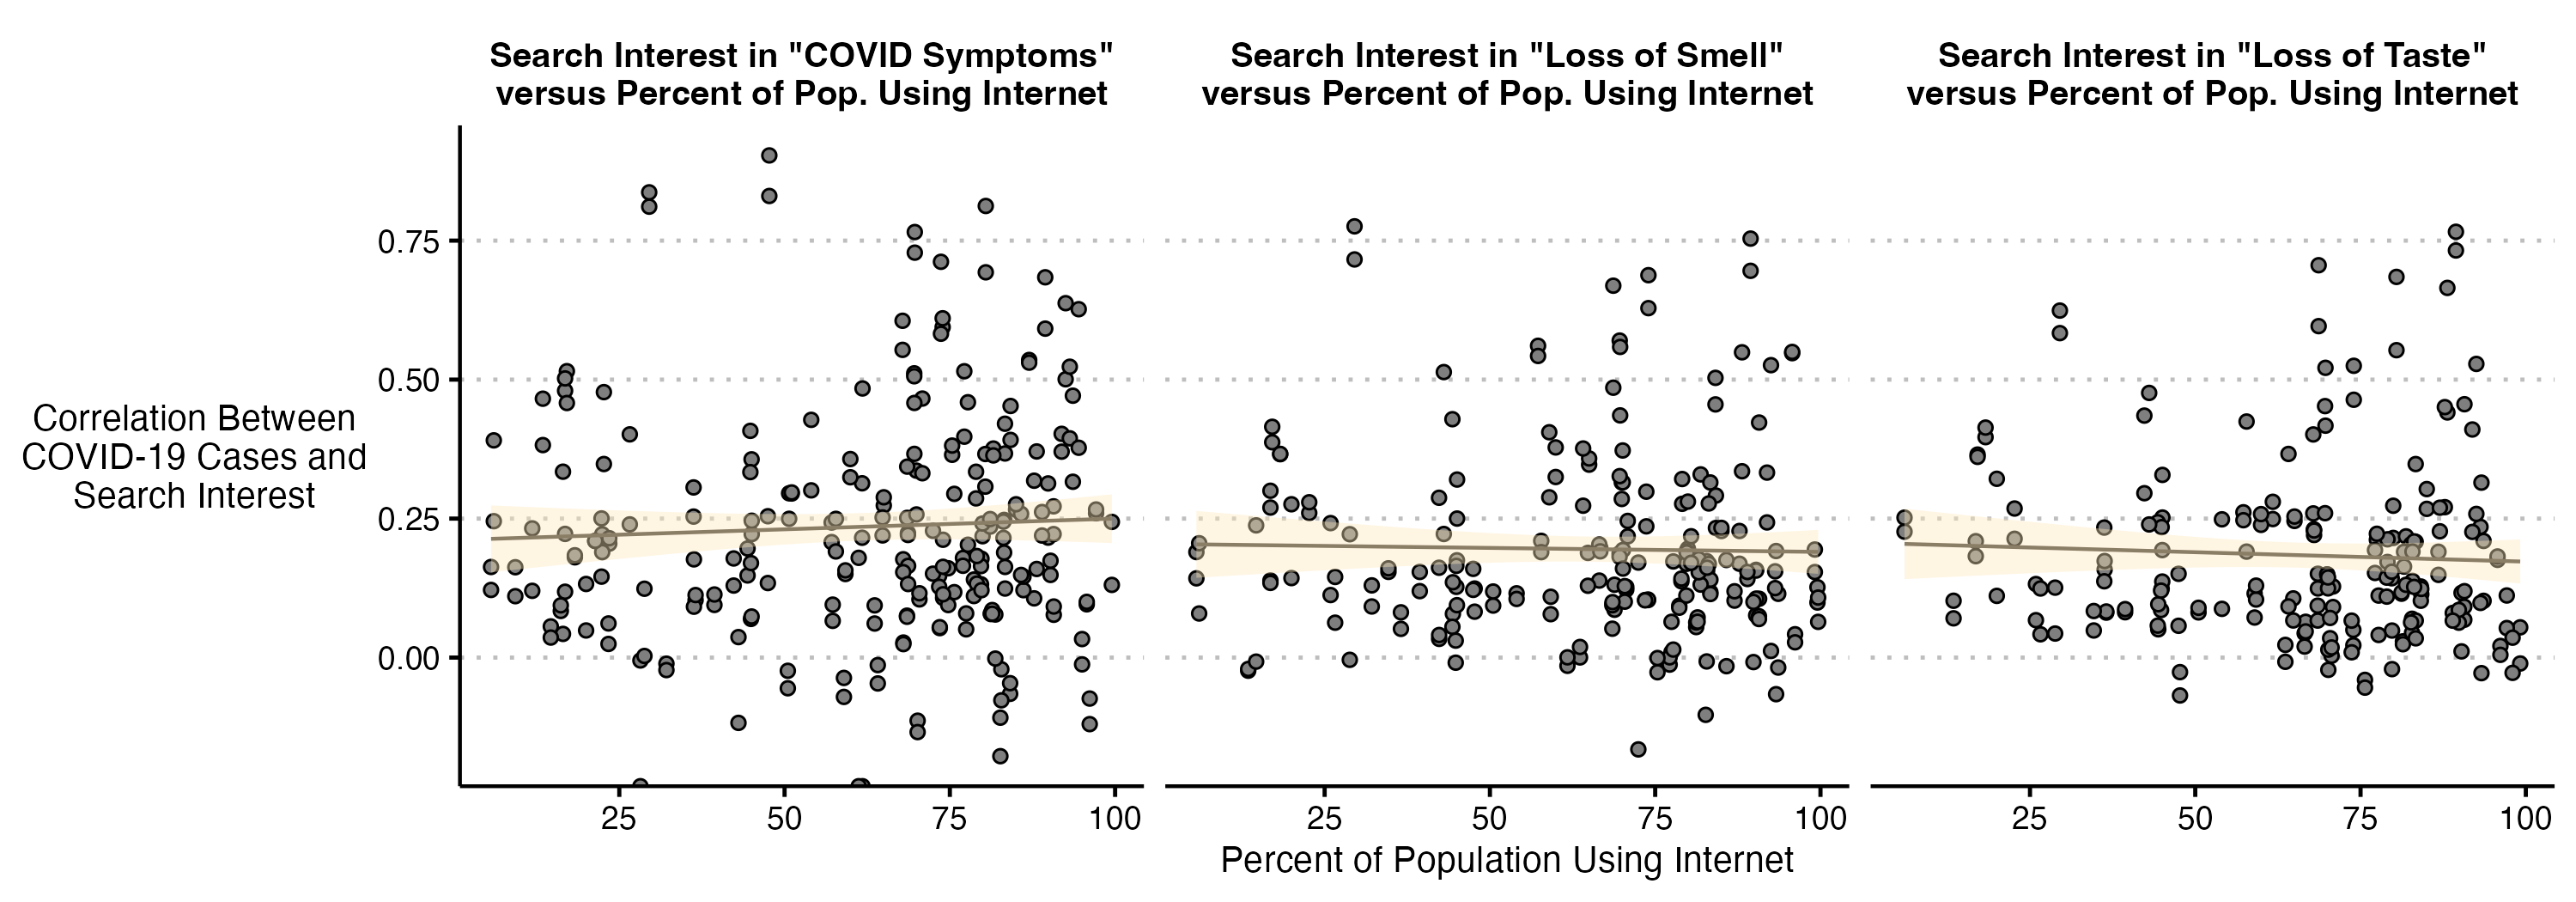
\includegraphics[width=1\textwidth]{figures/cor_internet_scatter.png}
    \caption{Scatterplots showing association between (1) correlation of search interest and COVID-19 cases and (2) percent of the population using internet, for search interest in ``COVID Symptoms'', ``Loss of Smell'', and ``Loss of Taste.''}
    \label{fig:cor_internet_scatter}
\end{figure}

\begin{figure}[H]
    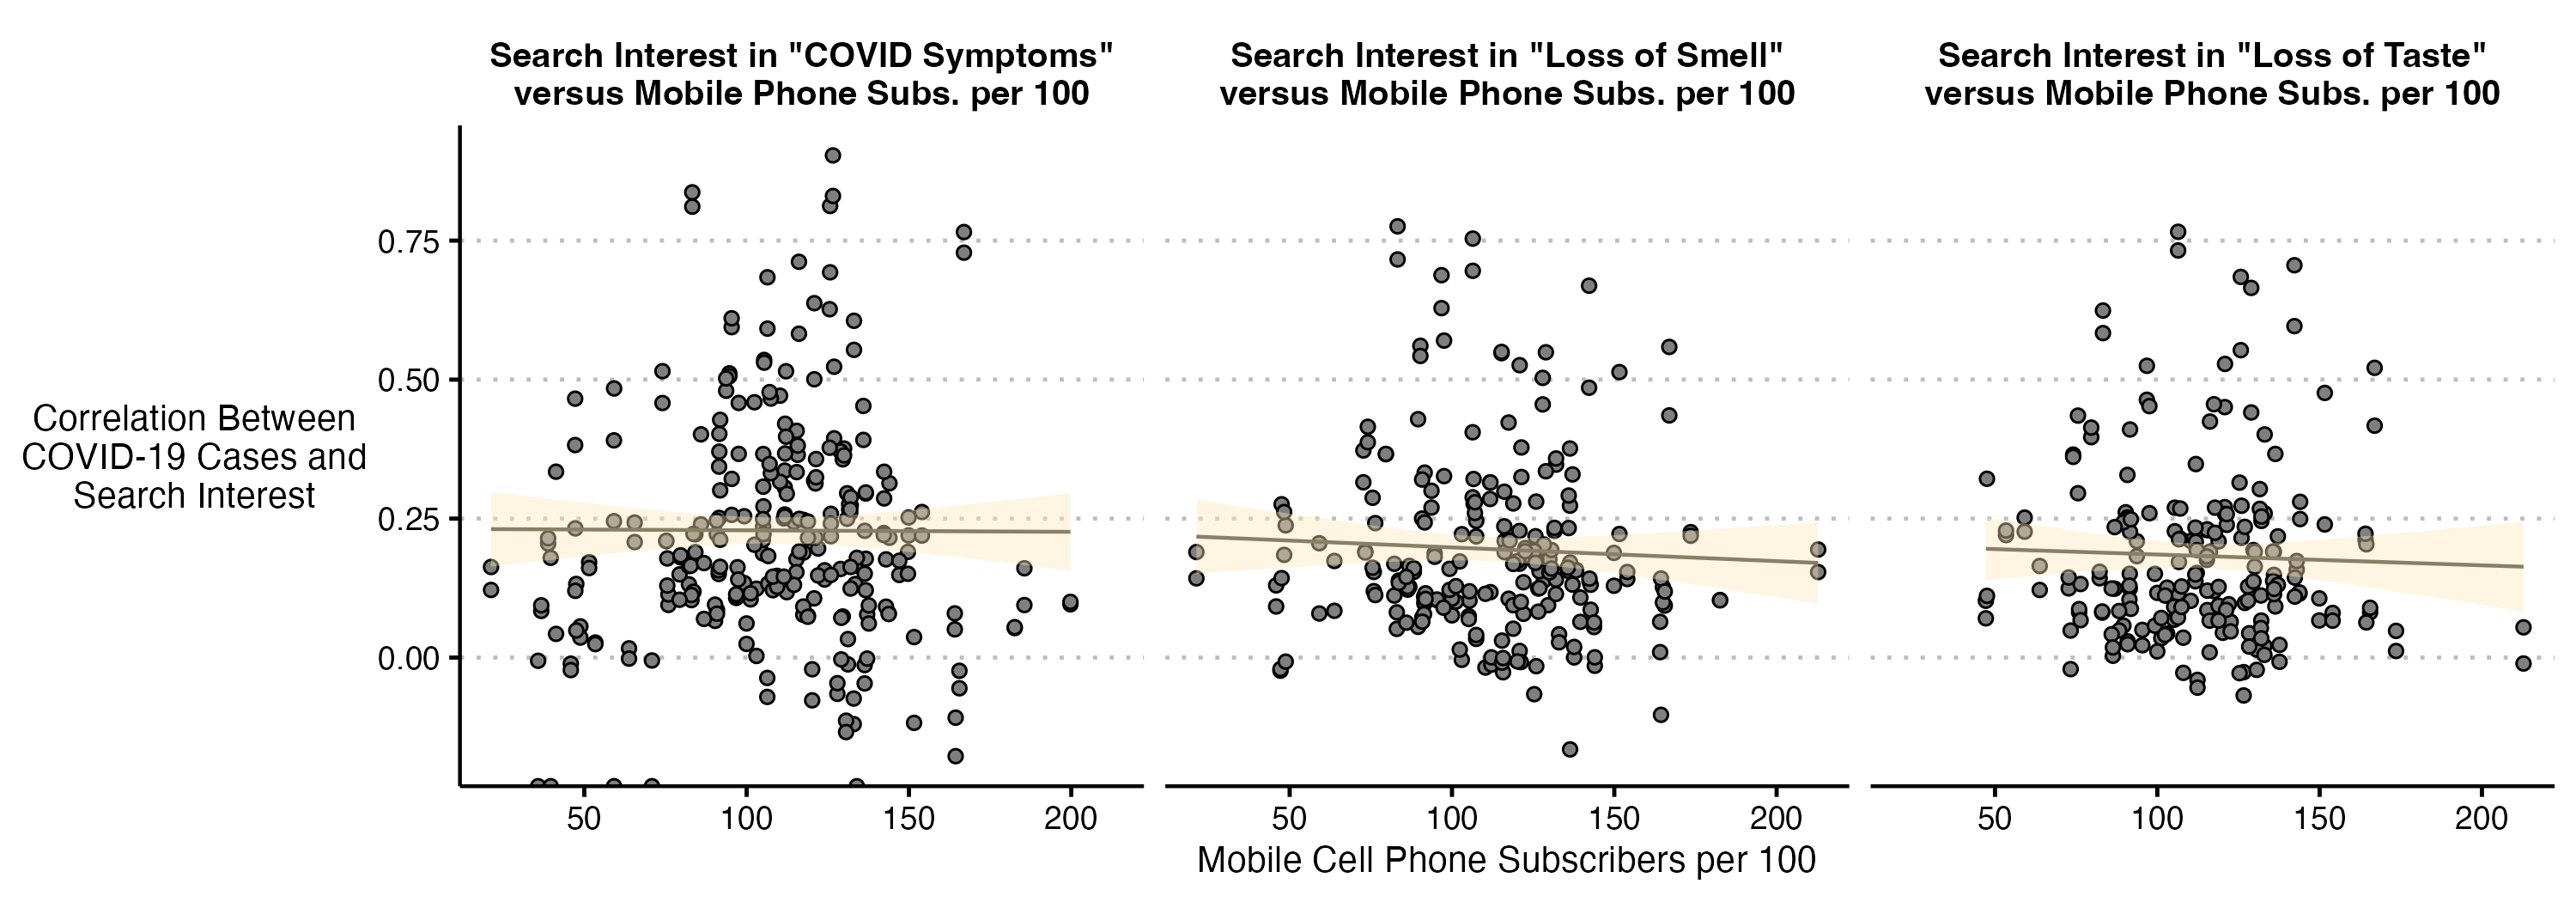
\includegraphics[width=1\textwidth]{figures/cor_mobilecell_scatter.png}
    \caption{Scatterplots showing association between (1) correlation of search interest and COVID-19 cases and (2) mobile cell phone subscribers per 100, logged, for search interest in ``COVID Symptoms'', ``Loss of Smell'', and ``Loss of Taste.''}
    \label{fig:cor_mobilecell_scatter}
\end{figure}

\begin{figure}[H]
    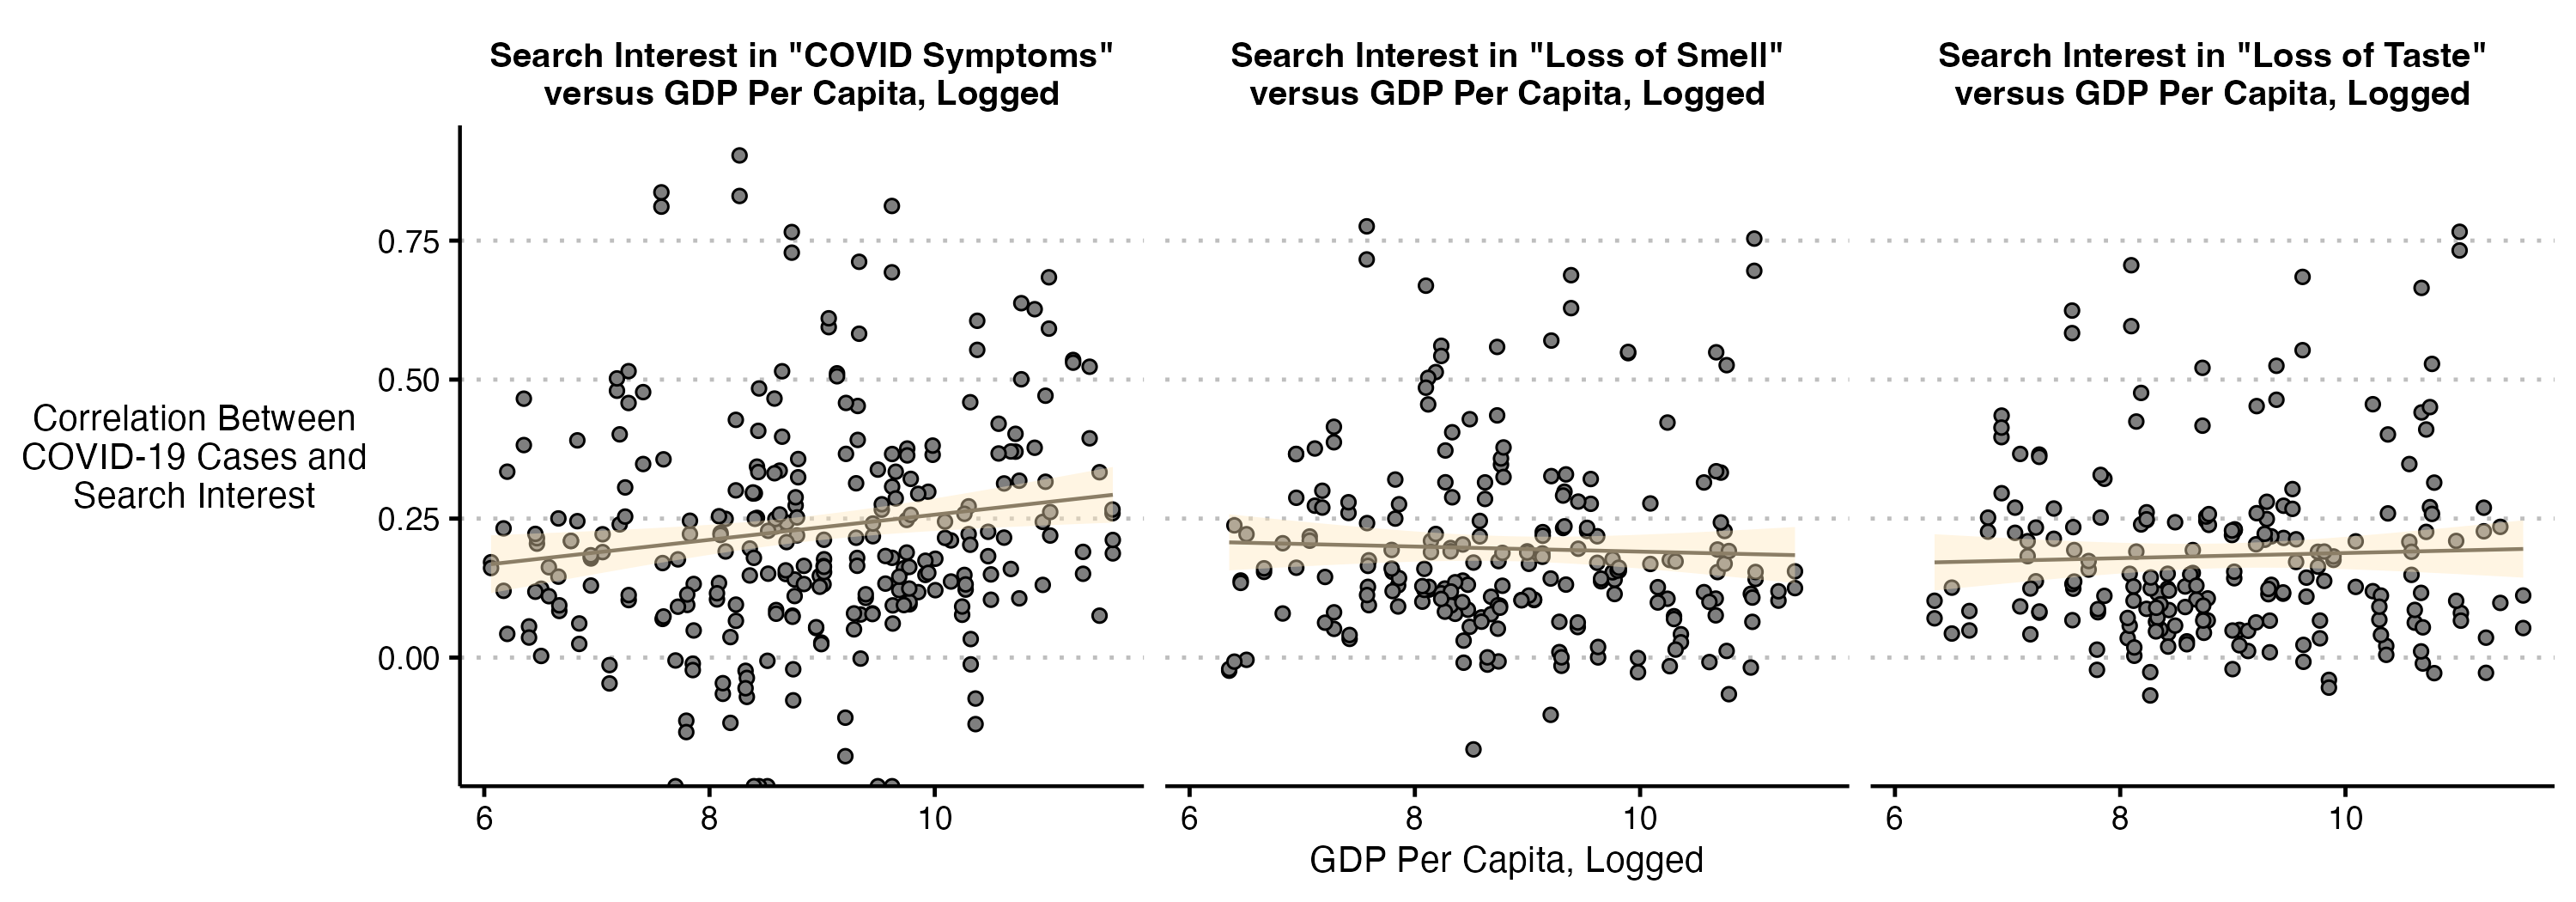
\includegraphics[width=1\textwidth]{figures/cor_gdp_scatter.png}
    \caption{Scatterplots showing association between (1) correlation of search interest and COVID-19 cases and (2) GDP per capita, logged, for search interest in ``COVID Symptoms'', ``Loss of Smell'', and ``Loss of Taste.''}
    \label{fig:cor_gdp_scatter}
\end{figure}

% --------------------------
\newpage
\section{Comparing correlation results using reported COVID-19 cases vs excess mortality}
\label{si:cor_cases_vs_excess}

%%%% Correlation betweetn two measures
\begin{figure}[H]
    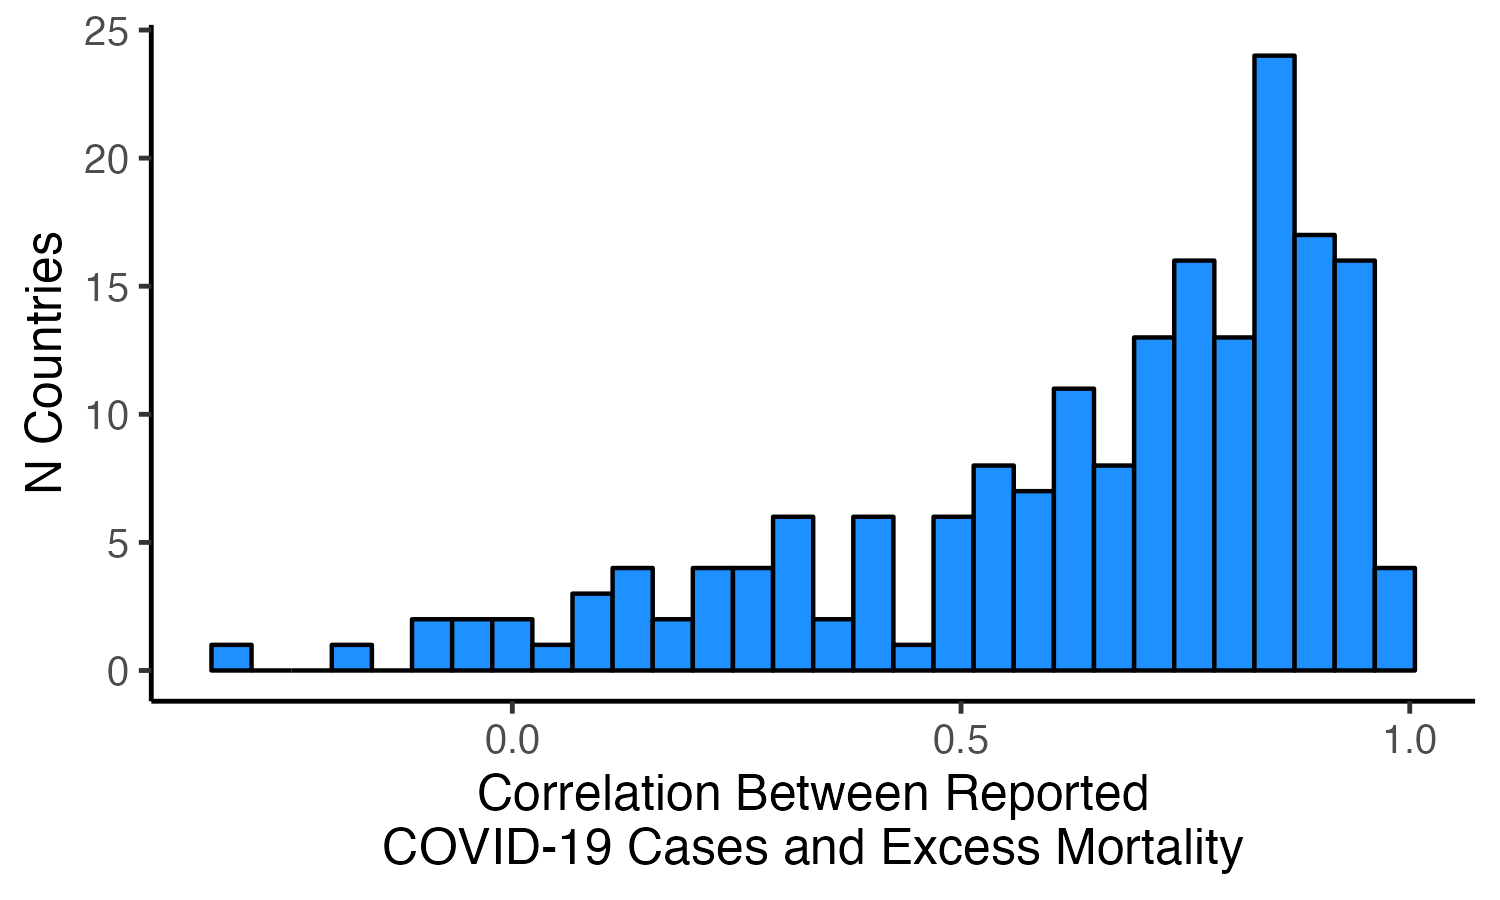
\includegraphics[width=1\textwidth]{figures/cor_cases_excess.png}
    \caption{\textcolor{black}{Distribution of within-country correlation between reported COVID-19 cases and excess mortality. Monthly data used from 2020-2021.}}
    \label{fig:cor_cases_excess}
\end{figure}

%%%% Boxplot Figures
\begin{figure}[H]
    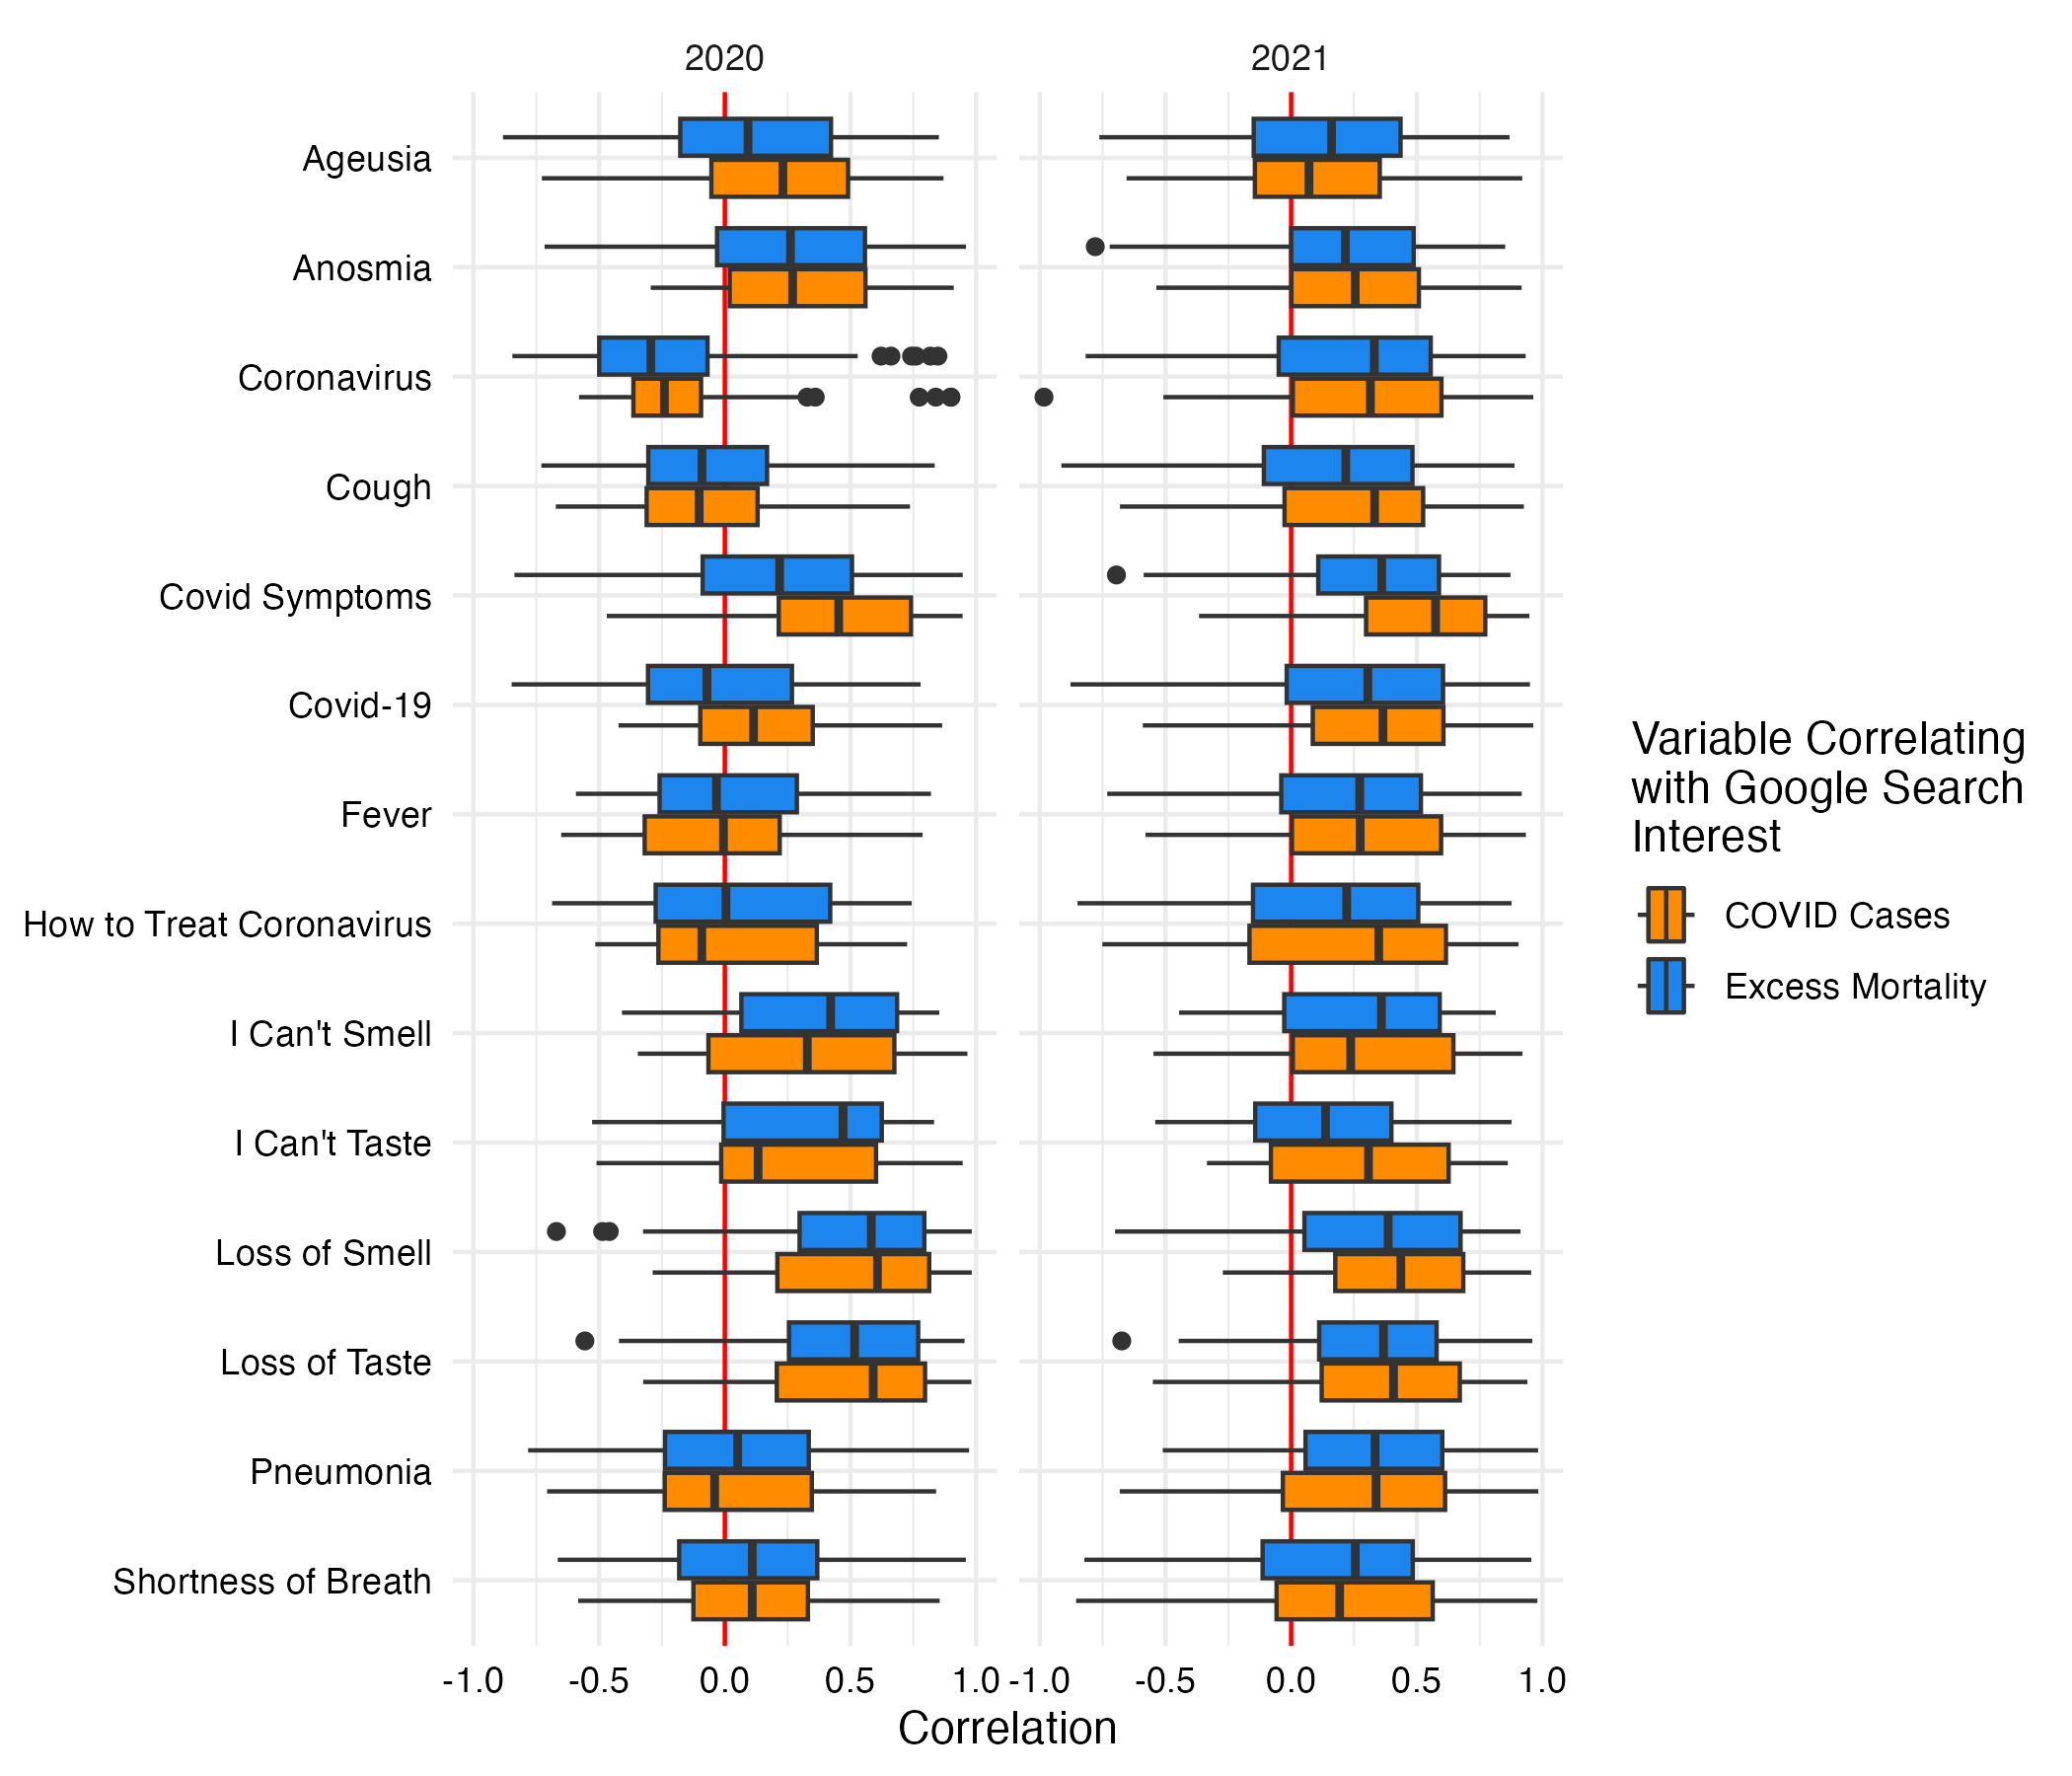
\includegraphics[width=1\textwidth]{figures/cases_excess_boxplot.png}
    \caption{Search interest correlating search interest across search terms and indicators of COVID (COVID cases and excess mortality). Panel A shows the correlation using 2020 data and panel B shows data using 2021 data. The boxplots include: center line, median; box limits, upper and lower quartiles; whiskers, 1.5x interquartile range; points beyond whiskers, outliers.}
    \label{fig:cases_excess_boxplot}
\end{figure}

\begin{figure}[H]
    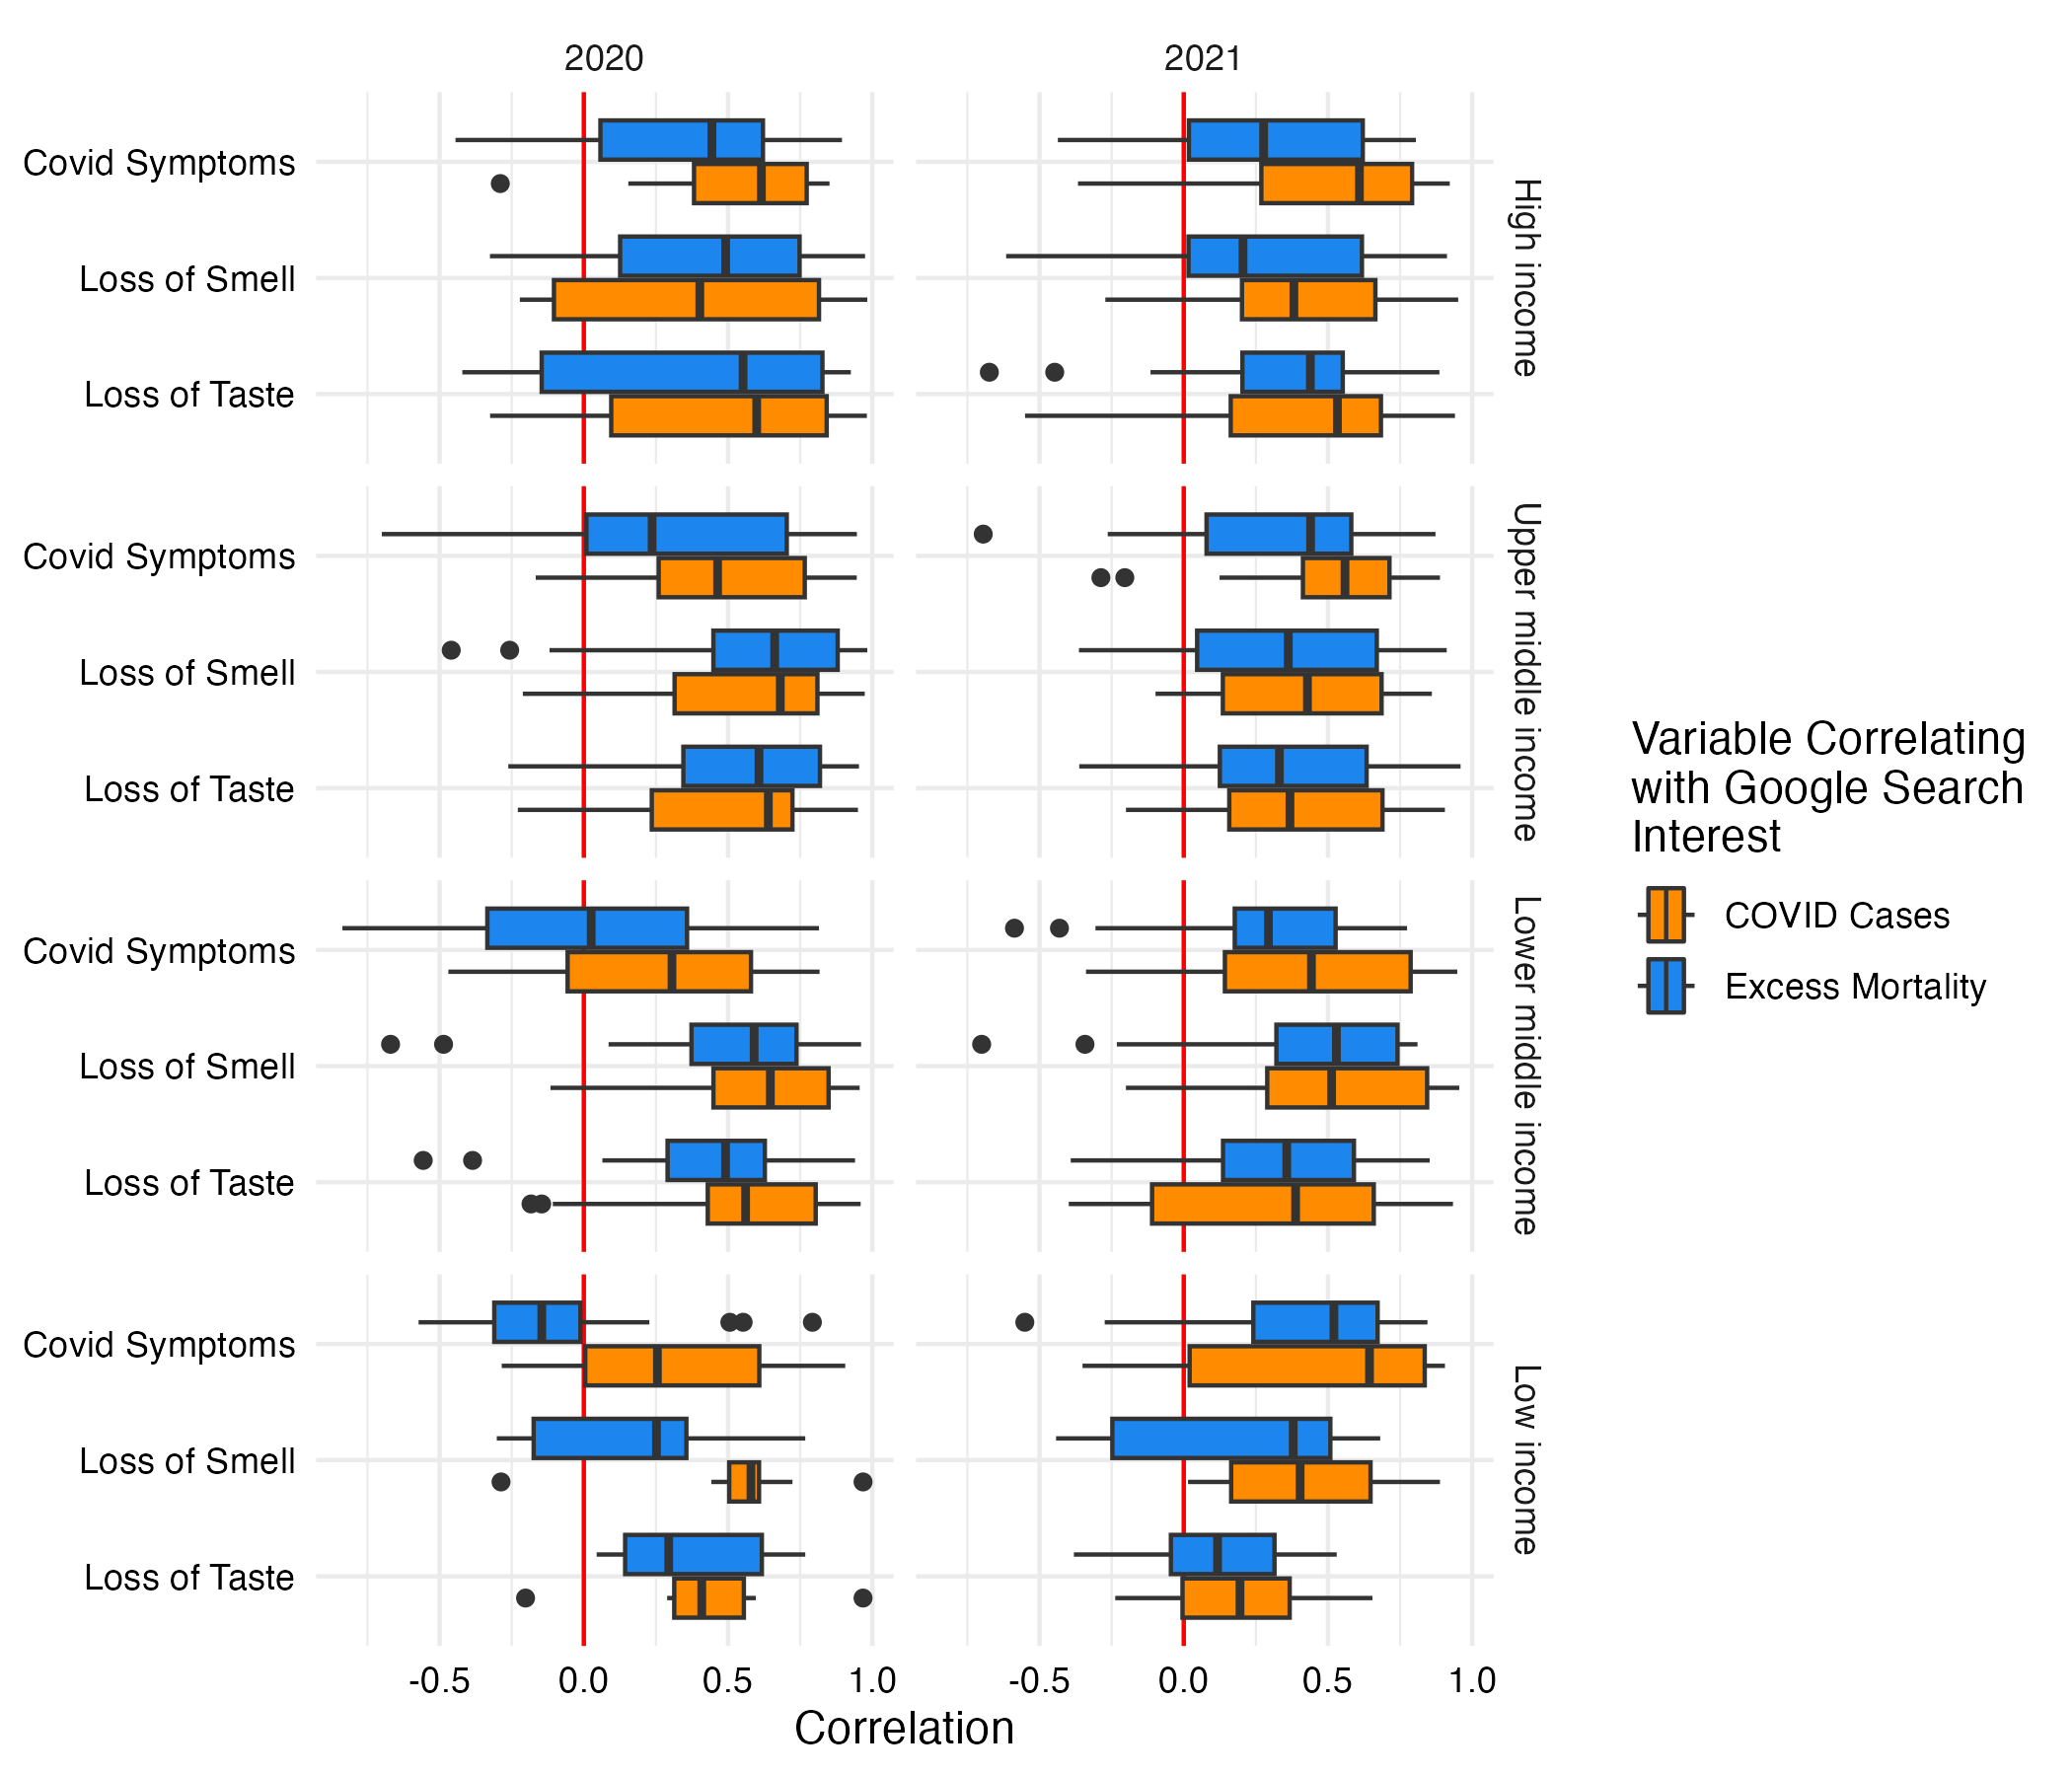
\includegraphics[width=1\textwidth]{figures/cases_excess_boxplot_income.png}
    \caption{\textcolor{black}{Search interest correlating search interest across search terms and indicators of COVID (COVID cases and excess mortality), by income level and using top Google search interest keywords.}}
    \label{fig:cases_excess_boxplot_income}
\end{figure}



%%%% Loss of Smell
\begin{table}[H]
\caption{Explaining correlation between COVID cases and search interest in Loss of Smell}
\label{tab:lm_cor_cases_monthly_loss_of_smell}
\centering

% Table created by stargazer v.5.2.3 by Marek Hlavac, Social Policy Institute. E-mail: marek.hlavac at gmail.com
% Date and time: Fri, Oct 13, 2023 - 09:00:12
% Requires LaTeX packages: dcolumn 
\begin{tabular}{@{\extracolsep{-15pt}}lD{.}{.}{-2} D{.}{.}{-2} D{.}{.}{-2} D{.}{.}{-2} D{.}{.}{-2} D{.}{.}{-2} D{.}{.}{-2} D{.}{.}{-2} } 
\\[-1.8ex]\hline 
\hline \\[-1.8ex] 
 & \multicolumn{8}{c}{\textit{Dependent variable:}} \\ 
\cline{2-9} 
\\[-1.8ex] & \multicolumn{8}{c}{Correlation} \\ 
\\[-1.8ex] & \multicolumn{1}{c}{(1)} & \multicolumn{1}{c}{(2)} & \multicolumn{1}{c}{(3)} & \multicolumn{1}{c}{(4)} & \multicolumn{1}{c}{(5)} & \multicolumn{1}{c}{(6)} & \multicolumn{1}{c}{(7)} & \multicolumn{1}{c}{(8)}\\ 
\hline \\[-1.8ex] 
 Total COVID-19 Cases, log & 0.01 &  &  &  &  &  & 0.02 & 0.02 \\ 
  & (0.01) &  &  &  &  &  & (0.02) & (0.02) \\ 
  Per Pop. Using Internet &  & -0.0004 &  &  &  &  &  & 0.002 \\ 
  &  & (0.001) &  &  &  &  &  & (0.003) \\ 
  Mobile Cell Sub. per 100 &  &  & 0.0004 &  &  &  &  & 0.001 \\ 
  &  &  & (0.001) &  &  &  &  & (0.001) \\ 
  GDP Per Cap, Log &  &  &  & -0.03 &  &  & -0.10 & -0.13^{*} \\ 
  &  &  &  & (0.02) &  &  & (0.06) & (0.08) \\ 
  Low Income &  &  &  &  & 0.04 &  & -0.07 & -0.01 \\ 
  &  &  &  &  & (0.10) &  & (0.24) & (0.25) \\ 
  Lower Middle Income &  &  &  &  & 0.11 &  & -0.01 & -0.002 \\ 
  &  &  &  &  & (0.07) &  & (0.17) & (0.17) \\ 
  Upper Middle Income &  &  &  &  & 0.02 &  & -0.04 & -0.07 \\ 
  &  &  &  &  & (0.07) &  & (0.11) & (0.11) \\ 
  Europe and Central Asia &  &  &  &  &  & 0.08 & 0.08 & 0.08 \\ 
  &  &  &  &  &  & (0.10) & (0.10) & (0.11) \\ 
  Latin America and Caribbean &  &  &  &  &  & 0.02 & 0.01 & 0.03 \\ 
  &  &  &  &  &  & (0.10) & (0.11) & (0.11) \\ 
  Middle East and North Africa &  &  &  &  &  & 0.12 & 0.13 & 0.10 \\ 
  &  &  &  &  &  & (0.11) & (0.11) & (0.12) \\ 
  North America &  &  &  &  &  & 0.53^{**} & 0.63^{***} & 0.67^{***} \\ 
  &  &  &  &  &  & (0.21) & (0.22) & (0.23) \\ 
  South Asia &  &  &  &  &  & 0.22 & 0.10 & 0.13 \\ 
  &  &  &  &  &  & (0.18) & (0.19) & (0.19) \\ 
  Sub-Saharan Africa &  &  &  &  &  & 0.005 & -0.11 & -0.08 \\ 
  &  &  &  &  &  & (0.11) & (0.12) & (0.13) \\ 
  Constant & 0.22 & 0.37^{***} & 0.31^{***} & 0.62^{***} & 0.31^{***} & 0.29^{***} & 1.00 & 0.99 \\ 
  & (0.18) & (0.08) & (0.10) & (0.20) & (0.05) & (0.09) & (0.65) & (0.68) \\ 
 \hline \\[-1.8ex] 
Observations & \multicolumn{1}{c}{109} & \multicolumn{1}{c}{104} & \multicolumn{1}{c}{108} & \multicolumn{1}{c}{105} & \multicolumn{1}{c}{107} & \multicolumn{1}{c}{109} & \multicolumn{1}{c}{105} & \multicolumn{1}{c}{103} \\ 
Adjusted R$^{2}$ & \multicolumn{1}{c}{-0.004} & \multicolumn{1}{c}{-0.01} & \multicolumn{1}{c}{-0.01} & \multicolumn{1}{c}{0.01} & \multicolumn{1}{c}{-0.002} & \multicolumn{1}{c}{0.03} & \multicolumn{1}{c}{0.08} & \multicolumn{1}{c}{0.07} \\ 
\hline 
\hline \\[-1.8ex] 
\end{tabular} 

\end{table}

\begin{table}[H]
\caption{Explaining correlation between excess mortality and search interest in Loss of Smell}
\label{tab:lm_cor_excess_monthly_loss_of_smell}
\centering

% Table created by stargazer v.5.2.3 by Marek Hlavac, Social Policy Institute. E-mail: marek.hlavac at gmail.com
% Date and time: Mon, Oct 09, 2023 - 17:10:57
% Requires LaTeX packages: dcolumn 
\begin{tabular}{@{\extracolsep{-15pt}}lD{.}{.}{-2} D{.}{.}{-2} D{.}{.}{-2} D{.}{.}{-2} D{.}{.}{-2} D{.}{.}{-2} D{.}{.}{-2} D{.}{.}{-2} } 
\\[-1.8ex]\hline 
\hline \\[-1.8ex] 
 & \multicolumn{8}{c}{\textit{Dependent variable:}} \\ 
\cline{2-9} 
\\[-1.8ex] & \multicolumn{8}{c}{Correlation} \\ 
\\[-1.8ex] & \multicolumn{1}{c}{(1)} & \multicolumn{1}{c}{(2)} & \multicolumn{1}{c}{(3)} & \multicolumn{1}{c}{(4)} & \multicolumn{1}{c}{(5)} & \multicolumn{1}{c}{(6)} & \multicolumn{1}{c}{(7)} & \multicolumn{1}{c}{(8)}\\ 
\hline \\[-1.8ex] 
 Total COVID-19 Cases, log & 0.05^{***} &  &  &  &  &  & 0.06^{***} & 0.06^{***} \\ 
  & (0.01) &  &  &  &  &  & (0.02) & (0.02) \\ 
  Per Pop. Using Internet &  & 0.002^{*} &  &  &  &  &  & -0.003 \\ 
  &  & (0.001) &  &  &  &  &  & (0.003) \\ 
  Mobile Cell Sub. per 100 &  &  & 0.001 &  &  &  &  & 0.001 \\ 
  &  &  & (0.001) &  &  &  &  & (0.001) \\ 
  GDP Per Cap, Log &  &  &  & 0.01 &  &  & -0.09 & -0.06 \\ 
  &  &  &  & (0.02) &  &  & (0.06) & (0.07) \\ 
  Low Income &  &  &  &  & -0.19^{*} &  & -0.04 & -0.06 \\ 
  &  &  &  &  & (0.11) &  & (0.23) & (0.24) \\ 
  Lower Middle Income &  &  &  &  & 0.06 &  & 0.08 & 0.07 \\ 
  &  &  &  &  & (0.07) &  & (0.16) & (0.16) \\ 
  Upper Middle Income &  &  &  &  & 0.07 &  & 0.06 & 0.07 \\ 
  &  &  &  &  & (0.07) &  & (0.11) & (0.11) \\ 
  Europe and Central Asia &  &  &  &  &  & 0.17^{*} & 0.19^{*} & 0.20^{*} \\ 
  &  &  &  &  &  & (0.10) & (0.10) & (0.10) \\ 
  Latin America and Caribbean &  &  &  &  &  & 0.06 & 0.09 & 0.10 \\ 
  &  &  &  &  &  & (0.11) & (0.11) & (0.11) \\ 
  Middle East and North Africa &  &  &  &  &  & 0.18 & 0.24^{**} & 0.26^{**} \\ 
  &  &  &  &  &  & (0.11) & (0.11) & (0.11) \\ 
  North America &  &  &  &  &  & 0.21 & 0.27 & 0.29 \\ 
  &  &  &  &  &  & (0.22) & (0.21) & (0.22) \\ 
  South Asia &  &  &  &  &  & -0.07 & -0.21 & -0.24 \\ 
  &  &  &  &  &  & (0.18) & (0.18) & (0.19) \\ 
  Sub-Saharan Africa &  &  &  &  &  & -0.15 & -0.13 & -0.14 \\ 
  &  &  &  &  &  & (0.11) & (0.12) & (0.12) \\ 
  Constant & -0.30^{*} & 0.23^{***} & 0.21^{**} & 0.29 & 0.35^{***} & 0.31^{***} & 0.27 & 0.12 \\ 
  & (0.18) & (0.08) & (0.11) & (0.21) & (0.05) & (0.09) & (0.62) & (0.66) \\ 
 \hline \\[-1.8ex] 
Observations & \multicolumn{1}{c}{109} & \multicolumn{1}{c}{104} & \multicolumn{1}{c}{108} & \multicolumn{1}{c}{105} & \multicolumn{1}{c}{107} & \multicolumn{1}{c}{109} & \multicolumn{1}{c}{105} & \multicolumn{1}{c}{103} \\ 
Adjusted R$^{2}$ & \multicolumn{1}{c}{0.11} & \multicolumn{1}{c}{0.02} & \multicolumn{1}{c}{0.01} & \multicolumn{1}{c}{-0.01} & \multicolumn{1}{c}{0.03} & \multicolumn{1}{c}{0.13} & \multicolumn{1}{c}{0.23} & \multicolumn{1}{c}{0.22} \\ 
\hline 
\hline \\[-1.8ex] 
\end{tabular} 

\end{table}

%%%% Loss of Taste
\begin{table}[H]
\caption{Explaining correlation between COVID cases and search interest in Loss of Taste}
\label{tab:lm_cor_cases_monthly_loss_of_taste}
\centering

% Table created by stargazer v.5.2.3 by Marek Hlavac, Social Policy Institute. E-mail: marek.hlavac at gmail.com
% Date and time: Mon, Oct 09, 2023 - 17:10:57
% Requires LaTeX packages: dcolumn 
\begin{tabular}{@{\extracolsep{-15pt}}lD{.}{.}{-2} D{.}{.}{-2} D{.}{.}{-2} D{.}{.}{-2} D{.}{.}{-2} D{.}{.}{-2} D{.}{.}{-2} D{.}{.}{-2} } 
\\[-1.8ex]\hline 
\hline \\[-1.8ex] 
 & \multicolumn{8}{c}{\textit{Dependent variable:}} \\ 
\cline{2-9} 
\\[-1.8ex] & \multicolumn{8}{c}{Correlation} \\ 
\\[-1.8ex] & \multicolumn{1}{c}{(1)} & \multicolumn{1}{c}{(2)} & \multicolumn{1}{c}{(3)} & \multicolumn{1}{c}{(4)} & \multicolumn{1}{c}{(5)} & \multicolumn{1}{c}{(6)} & \multicolumn{1}{c}{(7)} & \multicolumn{1}{c}{(8)}\\ 
\hline \\[-1.8ex] 
 Total COVID-19 Cases, log & 0.03^{*} &  &  &  &  &  & 0.03 & 0.03^{*} \\ 
  & (0.01) &  &  &  &  &  & (0.02) & (0.02) \\ 
  Per Pop. Using Internet &  & -0.0005 &  &  &  &  &  & -0.002 \\ 
  &  & (0.001) &  &  &  &  &  & (0.003) \\ 
  Mobile Cell Sub. per 100 &  &  & -0.001 &  &  &  &  & -0.001 \\ 
  &  &  & (0.001) &  &  &  &  & (0.001) \\ 
  GDP Per Cap, Log &  &  &  & 0.01 &  &  & 0.02 & 0.07 \\ 
  &  &  &  & (0.02) &  &  & (0.06) & (0.07) \\ 
  Low Income &  &  &  &  & -0.02 &  & 0.10 & 0.08 \\ 
  &  &  &  &  & (0.13) &  & (0.25) & (0.25) \\ 
  Lower Middle Income &  &  &  &  & 0.0000 &  & 0.09 & 0.08 \\ 
  &  &  &  &  & (0.07) &  & (0.17) & (0.17) \\ 
  Upper Middle Income &  &  &  &  & 0.01 &  & 0.07 & 0.11 \\ 
  &  &  &  &  & (0.07) &  & (0.12) & (0.12) \\ 
  Europe and Central Asia &  &  &  &  &  & -0.02 & -0.02 & -0.04 \\ 
  &  &  &  &  &  & (0.10) & (0.11) & (0.11) \\ 
  Latin America and Caribbean &  &  &  &  &  & -0.02 & 0.002 & -0.01 \\ 
  &  &  &  &  &  & (0.11) & (0.11) & (0.11) \\ 
  Middle East and North Africa &  &  &  &  &  & -0.12 & -0.09 & -0.04 \\ 
  &  &  &  &  &  & (0.12) & (0.12) & (0.13) \\ 
  North America &  &  &  &  &  & 0.49^{**} & 0.45^{*} & 0.39^{*} \\ 
  &  &  &  &  &  & (0.22) & (0.23) & (0.23) \\ 
  South Asia &  &  &  &  &  & 0.25 & 0.24 & 0.22 \\ 
  &  &  &  &  &  & (0.18) & (0.19) & (0.19) \\ 
  Sub-Saharan Africa &  &  &  &  &  & 0.02 & 0.09 & 0.11 \\ 
  &  &  &  &  &  & (0.11) & (0.13) & (0.13) \\ 
  Constant & -0.03 & 0.36^{***} & 0.45^{***} & 0.26 & 0.32^{***} & 0.33^{***} & -0.29 & -0.59 \\ 
  & (0.20) & (0.09) & (0.12) & (0.21) & (0.05) & (0.09) & (0.66) & (0.68) \\ 
 \hline \\[-1.8ex] 
Observations & \multicolumn{1}{c}{102} & \multicolumn{1}{c}{98} & \multicolumn{1}{c}{101} & \multicolumn{1}{c}{100} & \multicolumn{1}{c}{100} & \multicolumn{1}{c}{102} & \multicolumn{1}{c}{100} & \multicolumn{1}{c}{98} \\ 
Adjusted R$^{2}$ & \multicolumn{1}{c}{0.02} & \multicolumn{1}{c}{-0.01} & \multicolumn{1}{c}{0.001} & \multicolumn{1}{c}{-0.01} & \multicolumn{1}{c}{-0.03} & \multicolumn{1}{c}{0.05} & \multicolumn{1}{c}{0.03} & \multicolumn{1}{c}{0.04} \\ 
\hline 
\hline \\[-1.8ex] 
\end{tabular} 

\end{table}

\begin{table}[H]
\caption{Explaining correlation between excess mortality and search interest in Loss of Taste}
\label{tab:lm_cor_excess_monthly_loss_of_taste}
\centering

% Table created by stargazer v.5.2.3 by Marek Hlavac, Social Policy Institute. E-mail: marek.hlavac at gmail.com
% Date and time: Tue, Oct 03, 2023 - 06:36:14
% Requires LaTeX packages: dcolumn 
\begin{tabular}{@{\extracolsep{-15pt}}lD{.}{.}{-2} D{.}{.}{-2} D{.}{.}{-2} D{.}{.}{-2} D{.}{.}{-2} D{.}{.}{-2} D{.}{.}{-2} D{.}{.}{-2} } 
\\[-1.8ex]\hline 
\hline \\[-1.8ex] 
 & \multicolumn{8}{c}{\textit{Dependent variable:}} \\ 
\cline{2-9} 
\\[-1.8ex] & \multicolumn{8}{c}{Correlation} \\ 
\\[-1.8ex] & \multicolumn{1}{c}{(1)} & \multicolumn{1}{c}{(2)} & \multicolumn{1}{c}{(3)} & \multicolumn{1}{c}{(4)} & \multicolumn{1}{c}{(5)} & \multicolumn{1}{c}{(6)} & \multicolumn{1}{c}{(7)} & \multicolumn{1}{c}{(8)}\\ 
\hline \\[-1.8ex] 
 Total COVID-19 Cases, log & 0.03^{**} &  &  &  &  &  & 0.04^{**} & 0.04^{*} \\ 
  & (0.01) &  &  &  &  &  & (0.02) & (0.02) \\ 
  Per Pop. Using Internet &  & -0.0001 &  &  &  &  &  & -0.01^{**} \\ 
  &  & (0.001) &  &  &  &  &  & (0.003) \\ 
  Mobile Cell Sub. per 100 &  &  & 0.0003 &  &  &  &  & 0.001 \\ 
  &  &  & (0.001) &  &  &  &  & (0.001) \\ 
  GDP Per Cap, Log &  &  &  & 0.002 &  &  & -0.03 & 0.06 \\ 
  &  &  &  & (0.02) &  &  & (0.06) & (0.07) \\ 
  Low Income &  &  &  &  & -0.08 &  & -0.02 & -0.07 \\ 
  &  &  &  &  & (0.13) &  & (0.26) & (0.25) \\ 
  Lower Middle Income &  &  &  &  & 0.02 &  & 0.05 & 0.04 \\ 
  &  &  &  &  & (0.07) &  & (0.18) & (0.17) \\ 
  Upper Middle Income &  &  &  &  & 0.11 &  & 0.13 & 0.18 \\ 
  &  &  &  &  & (0.07) &  & (0.12) & (0.12) \\ 
  Europe and Central Asia &  &  &  &  &  & 0.16 & 0.16 & 0.18^{*} \\ 
  &  &  &  &  &  & (0.11) & (0.11) & (0.11) \\ 
  Latin America and Caribbean &  &  &  &  &  & 0.10 & 0.09 & 0.08 \\ 
  &  &  &  &  &  & (0.11) & (0.12) & (0.12) \\ 
  Middle East and North Africa &  &  &  &  &  & 0.13 & 0.15 & 0.25^{*} \\ 
  &  &  &  &  &  & (0.13) & (0.13) & (0.13) \\ 
  North America &  &  &  &  &  & 0.29 & 0.30 & 0.34 \\ 
  &  &  &  &  &  & (0.23) & (0.23) & (0.23) \\ 
  South Asia &  &  &  &  &  & 0.17 & 0.10 & 0.02 \\ 
  &  &  &  &  &  & (0.19) & (0.20) & (0.20) \\ 
  Sub-Saharan Africa &  &  &  &  &  & 0.06 & 0.11 & 0.06 \\ 
  &  &  &  &  &  & (0.12) & (0.13) & (0.13) \\ 
  Constant & -0.07 & 0.37^{***} & 0.33^{***} & 0.35^{*} & 0.33^{***} & 0.25^{***} & -0.08 & -0.56 \\ 
  & (0.20) & (0.09) & (0.12) & (0.21) & (0.05) & (0.09) & (0.68) & (0.69) \\ 
 \hline \\[-1.8ex] 
Observations & \multicolumn{1}{c}{102} & \multicolumn{1}{c}{98} & \multicolumn{1}{c}{101} & \multicolumn{1}{c}{100} & \multicolumn{1}{c}{100} & \multicolumn{1}{c}{102} & \multicolumn{1}{c}{100} & \multicolumn{1}{c}{98} \\ 
Adjusted R$^{2}$ & \multicolumn{1}{c}{0.04} & \multicolumn{1}{c}{-0.01} & \multicolumn{1}{c}{-0.01} & \multicolumn{1}{c}{-0.01} & \multicolumn{1}{c}{0.01} & \multicolumn{1}{c}{-0.02} & \multicolumn{1}{c}{0.01} & \multicolumn{1}{c}{0.06} \\ 
\hline 
\hline \\[-1.8ex] 
\end{tabular} 

\end{table}

%%%% COVID Cases
\begin{table}[H]
\caption{Explaining correlation between COVID cases and search interest in Loss of Taste}
\label{tab:lm_cor_cases_monthly_covid_symptoms}
\centering

% Table created by stargazer v.5.2.3 by Marek Hlavac, Social Policy Institute. E-mail: marek.hlavac at gmail.com
% Date and time: Mon, Oct 09, 2023 - 17:10:58
% Requires LaTeX packages: dcolumn 
\begin{tabular}{@{\extracolsep{-15pt}}lD{.}{.}{-2} D{.}{.}{-2} D{.}{.}{-2} D{.}{.}{-2} D{.}{.}{-2} D{.}{.}{-2} D{.}{.}{-2} D{.}{.}{-2} } 
\\[-1.8ex]\hline 
\hline \\[-1.8ex] 
 & \multicolumn{8}{c}{\textit{Dependent variable:}} \\ 
\cline{2-9} 
\\[-1.8ex] & \multicolumn{8}{c}{Correlation} \\ 
\\[-1.8ex] & \multicolumn{1}{c}{(1)} & \multicolumn{1}{c}{(2)} & \multicolumn{1}{c}{(3)} & \multicolumn{1}{c}{(4)} & \multicolumn{1}{c}{(5)} & \multicolumn{1}{c}{(6)} & \multicolumn{1}{c}{(7)} & \multicolumn{1}{c}{(8)}\\ 
\hline \\[-1.8ex] 
 Total COVID-19 Cases, log & 0.01 &  &  &  &  &  & 0.02 & 0.02 \\ 
  & (0.01) &  &  &  &  &  & (0.01) & (0.02) \\ 
  Per Pop. Using Internet &  & -0.0002 &  &  &  &  &  & -0.01^{**} \\ 
  &  & (0.001) &  &  &  &  &  & (0.003) \\ 
  Mobile Cell Sub. per 100 &  &  & 0.0003 &  &  &  &  & -0.001 \\ 
  &  &  & (0.001) &  &  &  &  & (0.001) \\ 
  GDP Per Cap, Log &  &  &  & 0.02 &  &  & -0.01 & 0.06 \\ 
  &  &  &  & (0.02) &  &  & (0.07) & (0.08) \\ 
  Low Income &  &  &  &  & -0.06 &  & -0.31 & -0.51^{*} \\ 
  &  &  &  &  & (0.09) &  & (0.25) & (0.26) \\ 
  Lower Middle Income &  &  &  &  & -0.12 &  & -0.25 & -0.35^{*} \\ 
  &  &  &  &  & (0.07) &  & (0.18) & (0.18) \\ 
  Upper Middle Income &  &  &  &  & 0.01 &  & -0.05 & -0.03 \\ 
  &  &  &  &  & (0.07) &  & (0.11) & (0.11) \\ 
  Europe and Central Asia &  &  &  &  &  & 0.06 & -0.05 & -0.04 \\ 
  &  &  &  &  &  & (0.09) & (0.10) & (0.10) \\ 
  Latin America and Caribbean &  &  &  &  &  & 0.11 & 0.07 & 0.04 \\ 
  &  &  &  &  &  & (0.09) & (0.10) & (0.10) \\ 
  Middle East and North Africa &  &  &  &  &  & -0.13 & -0.05 & 0.04 \\ 
  &  &  &  &  &  & (0.16) & (0.16) & (0.16) \\ 
  North America &  &  &  &  &  & 0.22 & 0.05 & 0.03 \\ 
  &  &  &  &  &  & (0.24) & (0.24) & (0.24) \\ 
  South Asia &  &  &  &  &  & 0.27 & 0.32^{*} & 0.24 \\ 
  &  &  &  &  &  & (0.17) & (0.17) & (0.18) \\ 
  Sub-Saharan Africa &  &  &  &  &  & 0.14 & 0.29^{**} & 0.21^{*} \\ 
  &  &  &  &  &  & (0.09) & (0.11) & (0.12) \\ 
  Constant & 0.25 & 0.40^{***} & 0.35^{***} & 0.24 & 0.42^{***} & 0.29^{***} & 0.28 & 0.26 \\ 
  & (0.16) & (0.07) & (0.09) & (0.19) & (0.05) & (0.08) & (0.69) & (0.70) \\ 
 \hline \\[-1.8ex] 
Observations & \multicolumn{1}{c}{129} & \multicolumn{1}{c}{124} & \multicolumn{1}{c}{128} & \multicolumn{1}{c}{126} & \multicolumn{1}{c}{127} & \multicolumn{1}{c}{129} & \multicolumn{1}{c}{126} & \multicolumn{1}{c}{123} \\ 
Adjusted R$^{2}$ & \multicolumn{1}{c}{-0.002} & \multicolumn{1}{c}{-0.01} & \multicolumn{1}{c}{-0.01} & \multicolumn{1}{c}{-0.003} & \multicolumn{1}{c}{0.01} & \multicolumn{1}{c}{0.01} & \multicolumn{1}{c}{0.06} & \multicolumn{1}{c}{0.10} \\ 
\hline 
\hline \\[-1.8ex] 
\end{tabular} 

\end{table}

\begin{table}[H]
\caption{Explaining correlation between excess mortality and search interest in Loss of Taste}
\label{tab:lm_cor_excess_monthly_covid_symptoms}
\centering

% Table created by stargazer v.5.2.3 by Marek Hlavac, Social Policy Institute. E-mail: marek.hlavac at gmail.com
% Date and time: Mon, Oct 09, 2023 - 17:10:59
% Requires LaTeX packages: dcolumn 
\begin{tabular}{@{\extracolsep{-15pt}}lD{.}{.}{-2} D{.}{.}{-2} D{.}{.}{-2} D{.}{.}{-2} D{.}{.}{-2} D{.}{.}{-2} D{.}{.}{-2} D{.}{.}{-2} } 
\\[-1.8ex]\hline 
\hline \\[-1.8ex] 
 & \multicolumn{8}{c}{\textit{Dependent variable:}} \\ 
\cline{2-9} 
\\[-1.8ex] & \multicolumn{8}{c}{Correlation} \\ 
\\[-1.8ex] & \multicolumn{1}{c}{(1)} & \multicolumn{1}{c}{(2)} & \multicolumn{1}{c}{(3)} & \multicolumn{1}{c}{(4)} & \multicolumn{1}{c}{(5)} & \multicolumn{1}{c}{(6)} & \multicolumn{1}{c}{(7)} & \multicolumn{1}{c}{(8)}\\ 
\hline \\[-1.8ex] 
 Total COVID-19 Cases, log & 0.03^{***} &  &  &  &  &  & 0.03^{**} & 0.03^{*} \\ 
  & (0.01) &  &  &  &  &  & (0.01) & (0.02) \\ 
  Per Pop. Using Internet &  & 0.002 &  &  &  &  &  & -0.01 \\ 
  &  & (0.001) &  &  &  &  &  & (0.003) \\ 
  Mobile Cell Sub. per 100 &  &  & 0.001 &  &  &  &  & -0.0004 \\ 
  &  &  & (0.001) &  &  &  &  & (0.001) \\ 
  GDP Per Cap, Log &  &  &  & 0.04^{*} &  &  & -0.05 & 0.02 \\ 
  &  &  &  & (0.02) &  &  & (0.07) & (0.08) \\ 
  Low Income &  &  &  &  & -0.15 &  & -0.32 & -0.42 \\ 
  &  &  &  &  & (0.09) &  & (0.26) & (0.27) \\ 
  Lower Middle Income &  &  &  &  & -0.18^{**} &  & -0.27 & -0.33^{*} \\ 
  &  &  &  &  & (0.07) &  & (0.18) & (0.19) \\ 
  Upper Middle Income &  &  &  &  & 0.01 &  & -0.04 & -0.01 \\ 
  &  &  &  &  & (0.07) &  & (0.11) & (0.12) \\ 
  Europe and Central Asia &  &  &  &  &  & 0.26^{***} & 0.13 & 0.13 \\ 
  &  &  &  &  &  & (0.09) & (0.10) & (0.10) \\ 
  Latin America and Caribbean &  &  &  &  &  & 0.23^{**} & 0.20^{**} & 0.16 \\ 
  &  &  &  &  &  & (0.10) & (0.10) & (0.11) \\ 
  Middle East and North Africa &  &  &  &  &  & 0.12 & 0.18 & 0.23 \\ 
  &  &  &  &  &  & (0.16) & (0.16) & (0.17) \\ 
  North America &  &  &  &  &  & 0.34 & 0.16 & 0.14 \\ 
  &  &  &  &  &  & (0.24) & (0.24) & (0.25) \\ 
  South Asia &  &  &  &  &  & 0.22 & 0.22 & 0.15 \\ 
  &  &  &  &  &  & (0.18) & (0.18) & (0.18) \\ 
  Sub-Saharan Africa &  &  &  &  &  & 0.16 & 0.26^{**} & 0.19 \\ 
  &  &  &  &  &  & (0.10) & (0.11) & (0.12) \\ 
  Constant & -0.18 & 0.16^{**} & 0.14 & -0.08 & 0.32^{***} & 0.07 & 0.18 & 0.11 \\ 
  & (0.16) & (0.07) & (0.10) & (0.19) & (0.05) & (0.08) & (0.69) & (0.72) \\ 
 \hline \\[-1.8ex] 
Observations & \multicolumn{1}{c}{129} & \multicolumn{1}{c}{124} & \multicolumn{1}{c}{128} & \multicolumn{1}{c}{126} & \multicolumn{1}{c}{127} & \multicolumn{1}{c}{129} & \multicolumn{1}{c}{126} & \multicolumn{1}{c}{123} \\ 
Adjusted R$^{2}$ & \multicolumn{1}{c}{0.05} & \multicolumn{1}{c}{0.01} & \multicolumn{1}{c}{0.003} & \multicolumn{1}{c}{0.02} & \multicolumn{1}{c}{0.05} & \multicolumn{1}{c}{0.02} & \multicolumn{1}{c}{0.08} & \multicolumn{1}{c}{0.07} \\ 
\hline 
\hline \\[-1.8ex] 
\end{tabular} 

\end{table}

% --------------------------
\newpage
\section{Association of containment policies with search interest: event study results}
\label{si:contain_es}

\begin{figure}[H]
    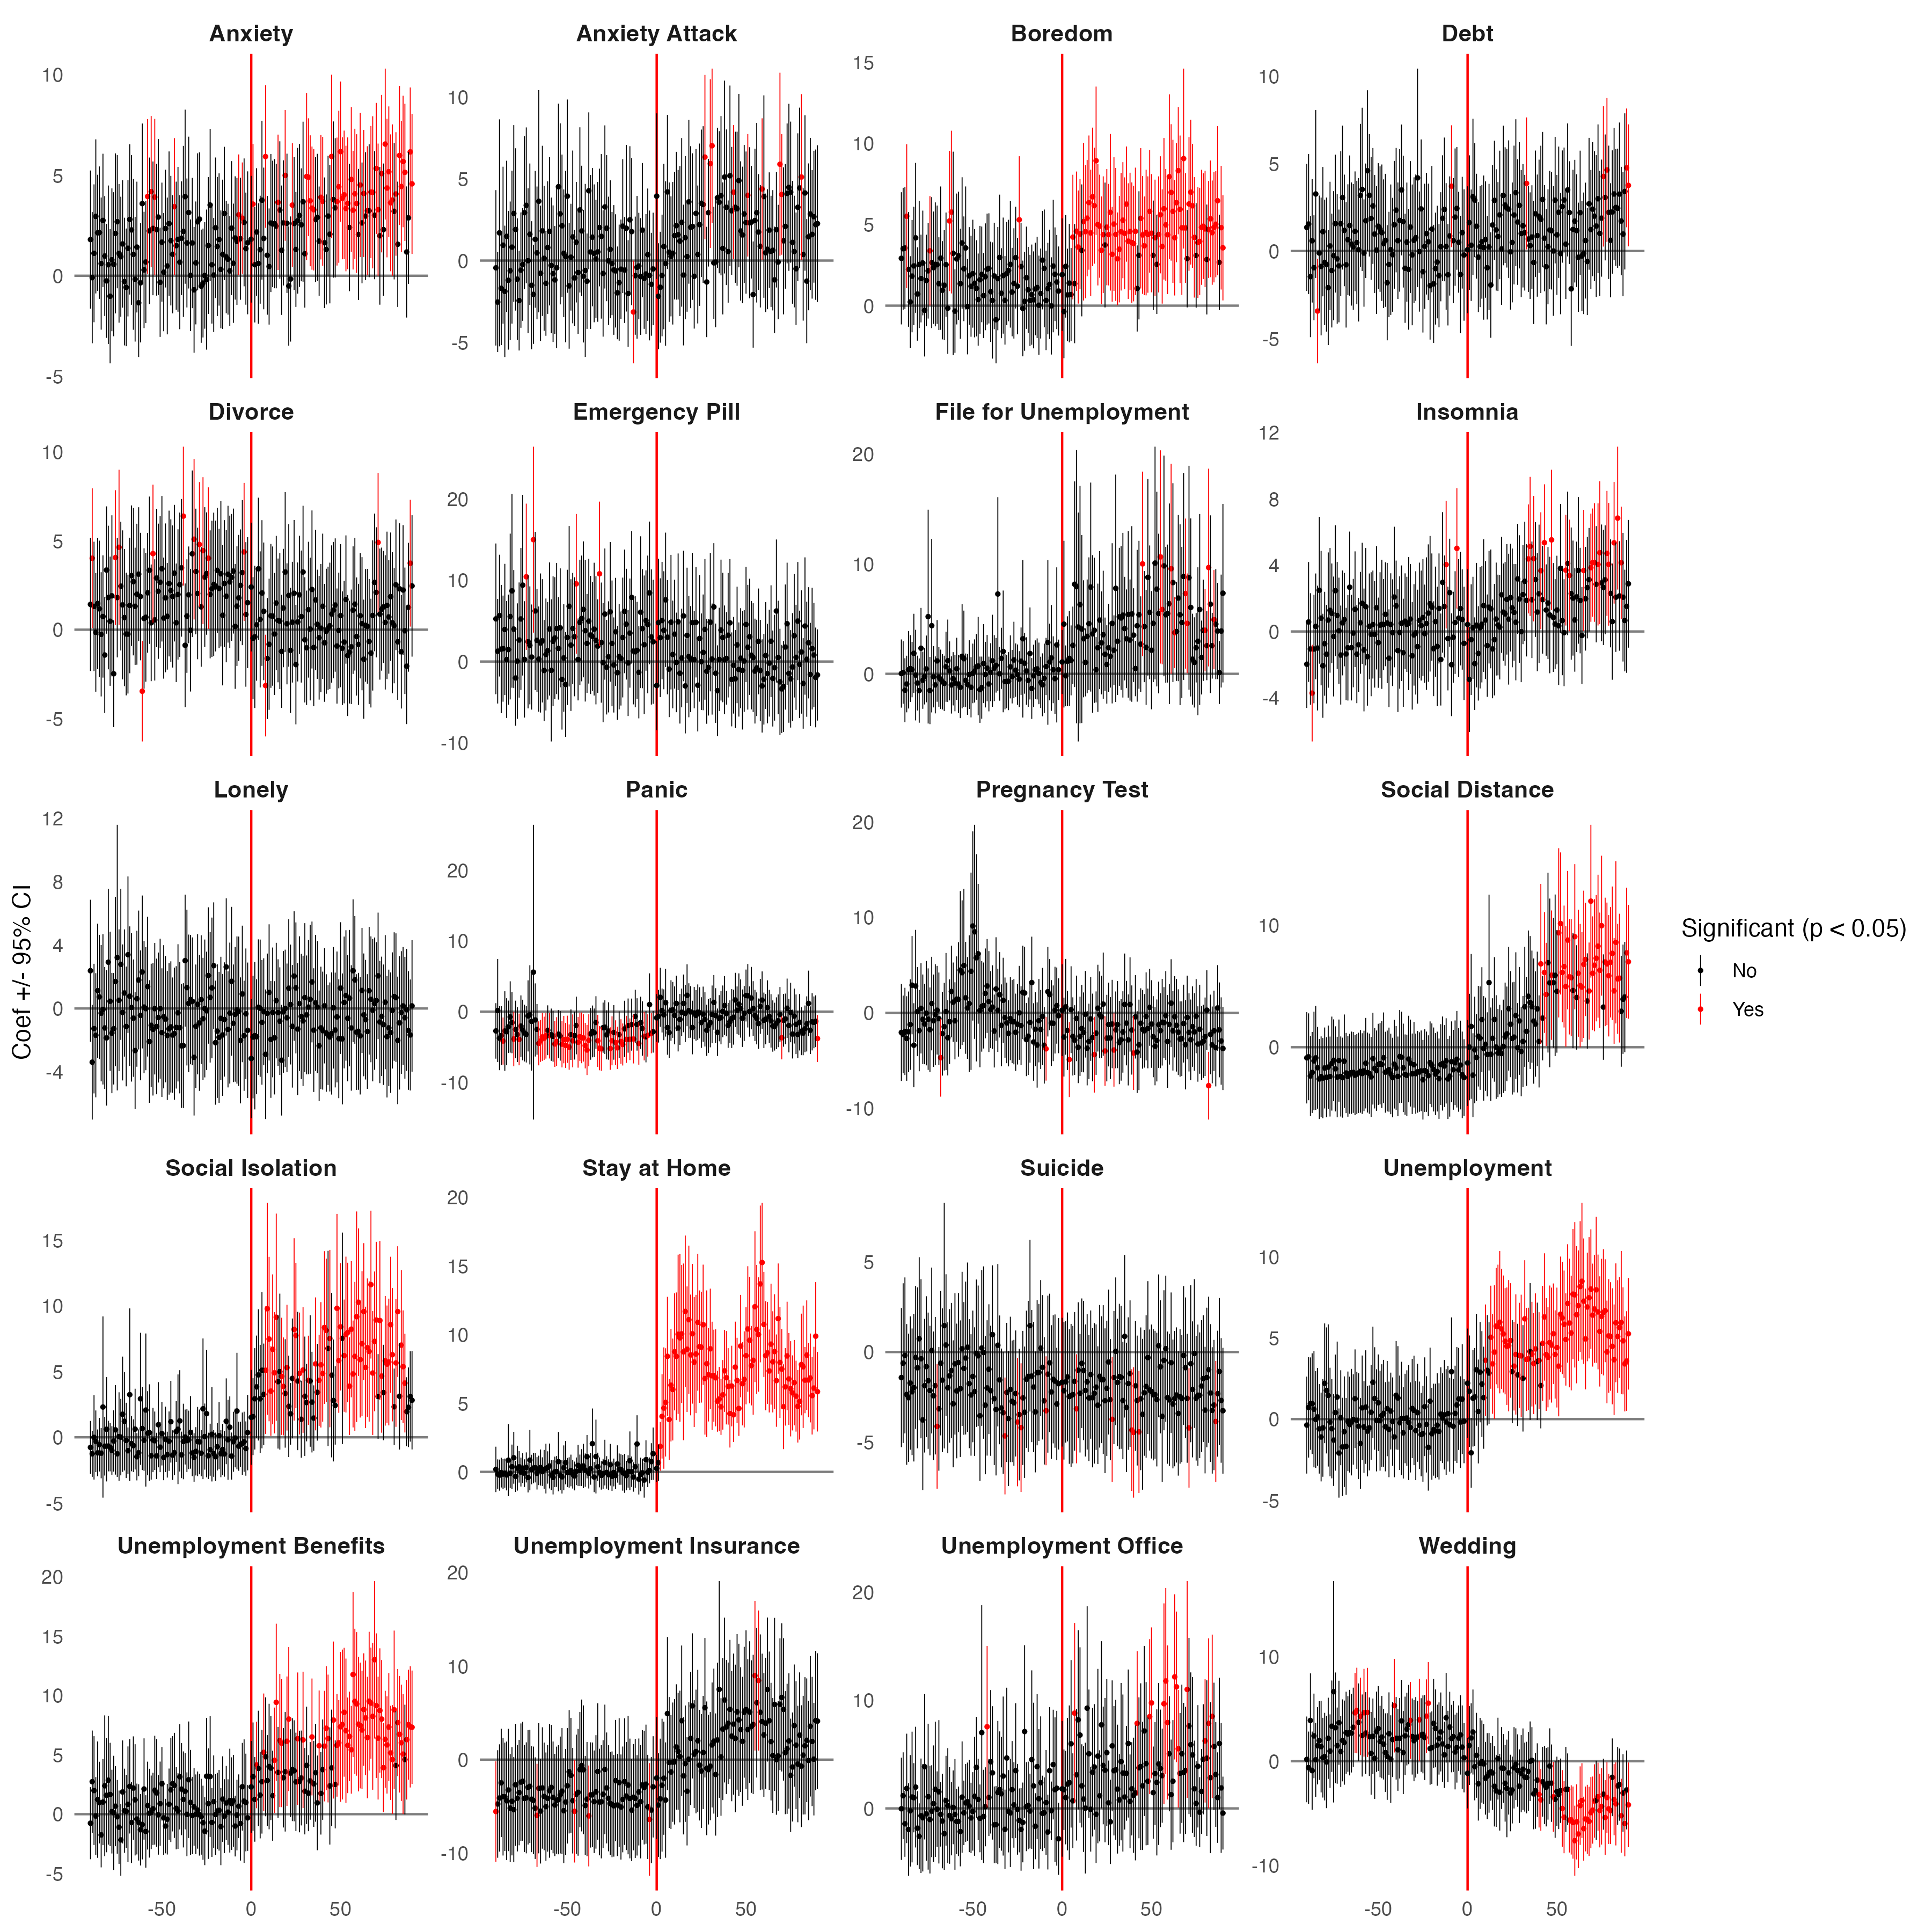
\includegraphics[width=1\textwidth]{figures/es_global_90days.png}
    \caption{Event study examining the association of containment policies with search interest. 95\% confidence intervals shown for each coefficient.}
    \label{fig:contain_es}
\end{figure}

% --------------------------
\newpage
\section{Association of Containment Policies with Search Interest: Sensitivity Analysis Across Different Day Thresholds}
\label{si:lockdown_impact_diffdays}

% --------------------------
%\newpage
\subsection{30 day threshold}

\begin{figure}[H]
    \centering
    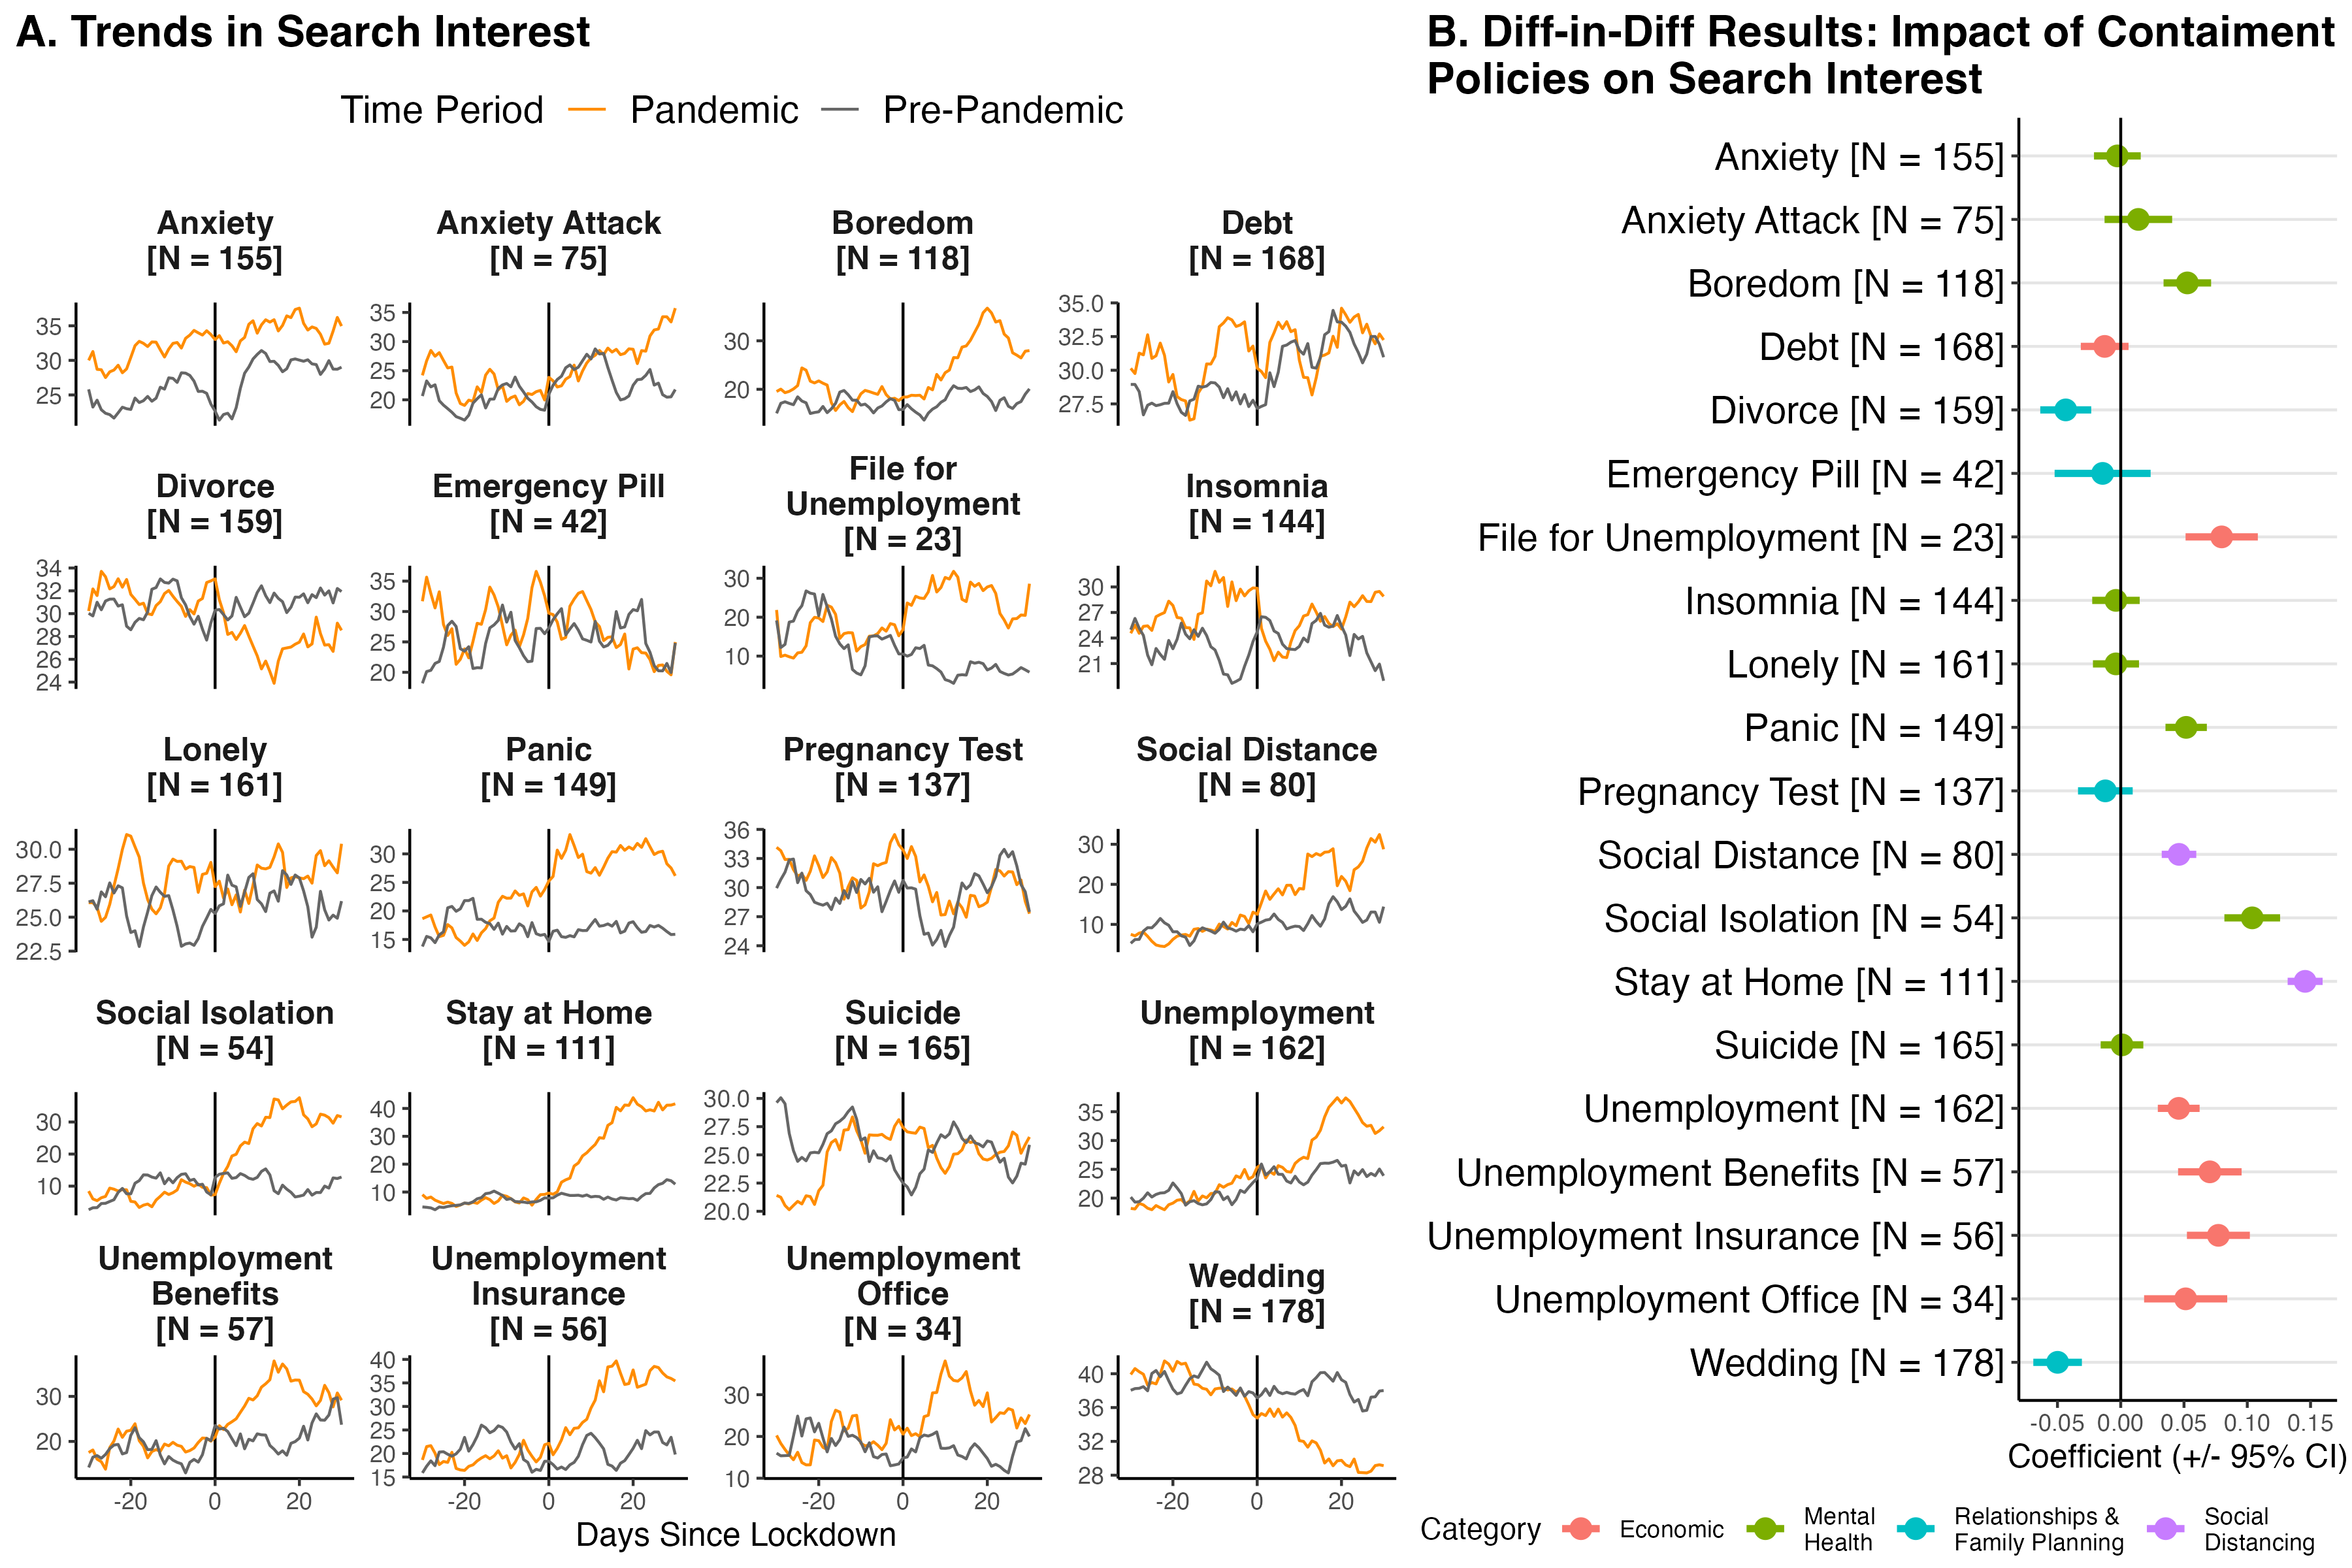
\includegraphics[width=0.85\textwidth]{figures/did_overall_30.png}
    \caption{Association of COVID-19 policies with search interest: results pooling all countries. Point estimates and 95\% confidence intervals are shown. To more clearly show trends, the seven day moving average of search interest is shown in panel A. `N' indicates the number of countries with available data.}
    \label{fig:lockdown_impact_30}
\end{figure}

\begin{figure}[H]
    \centering
    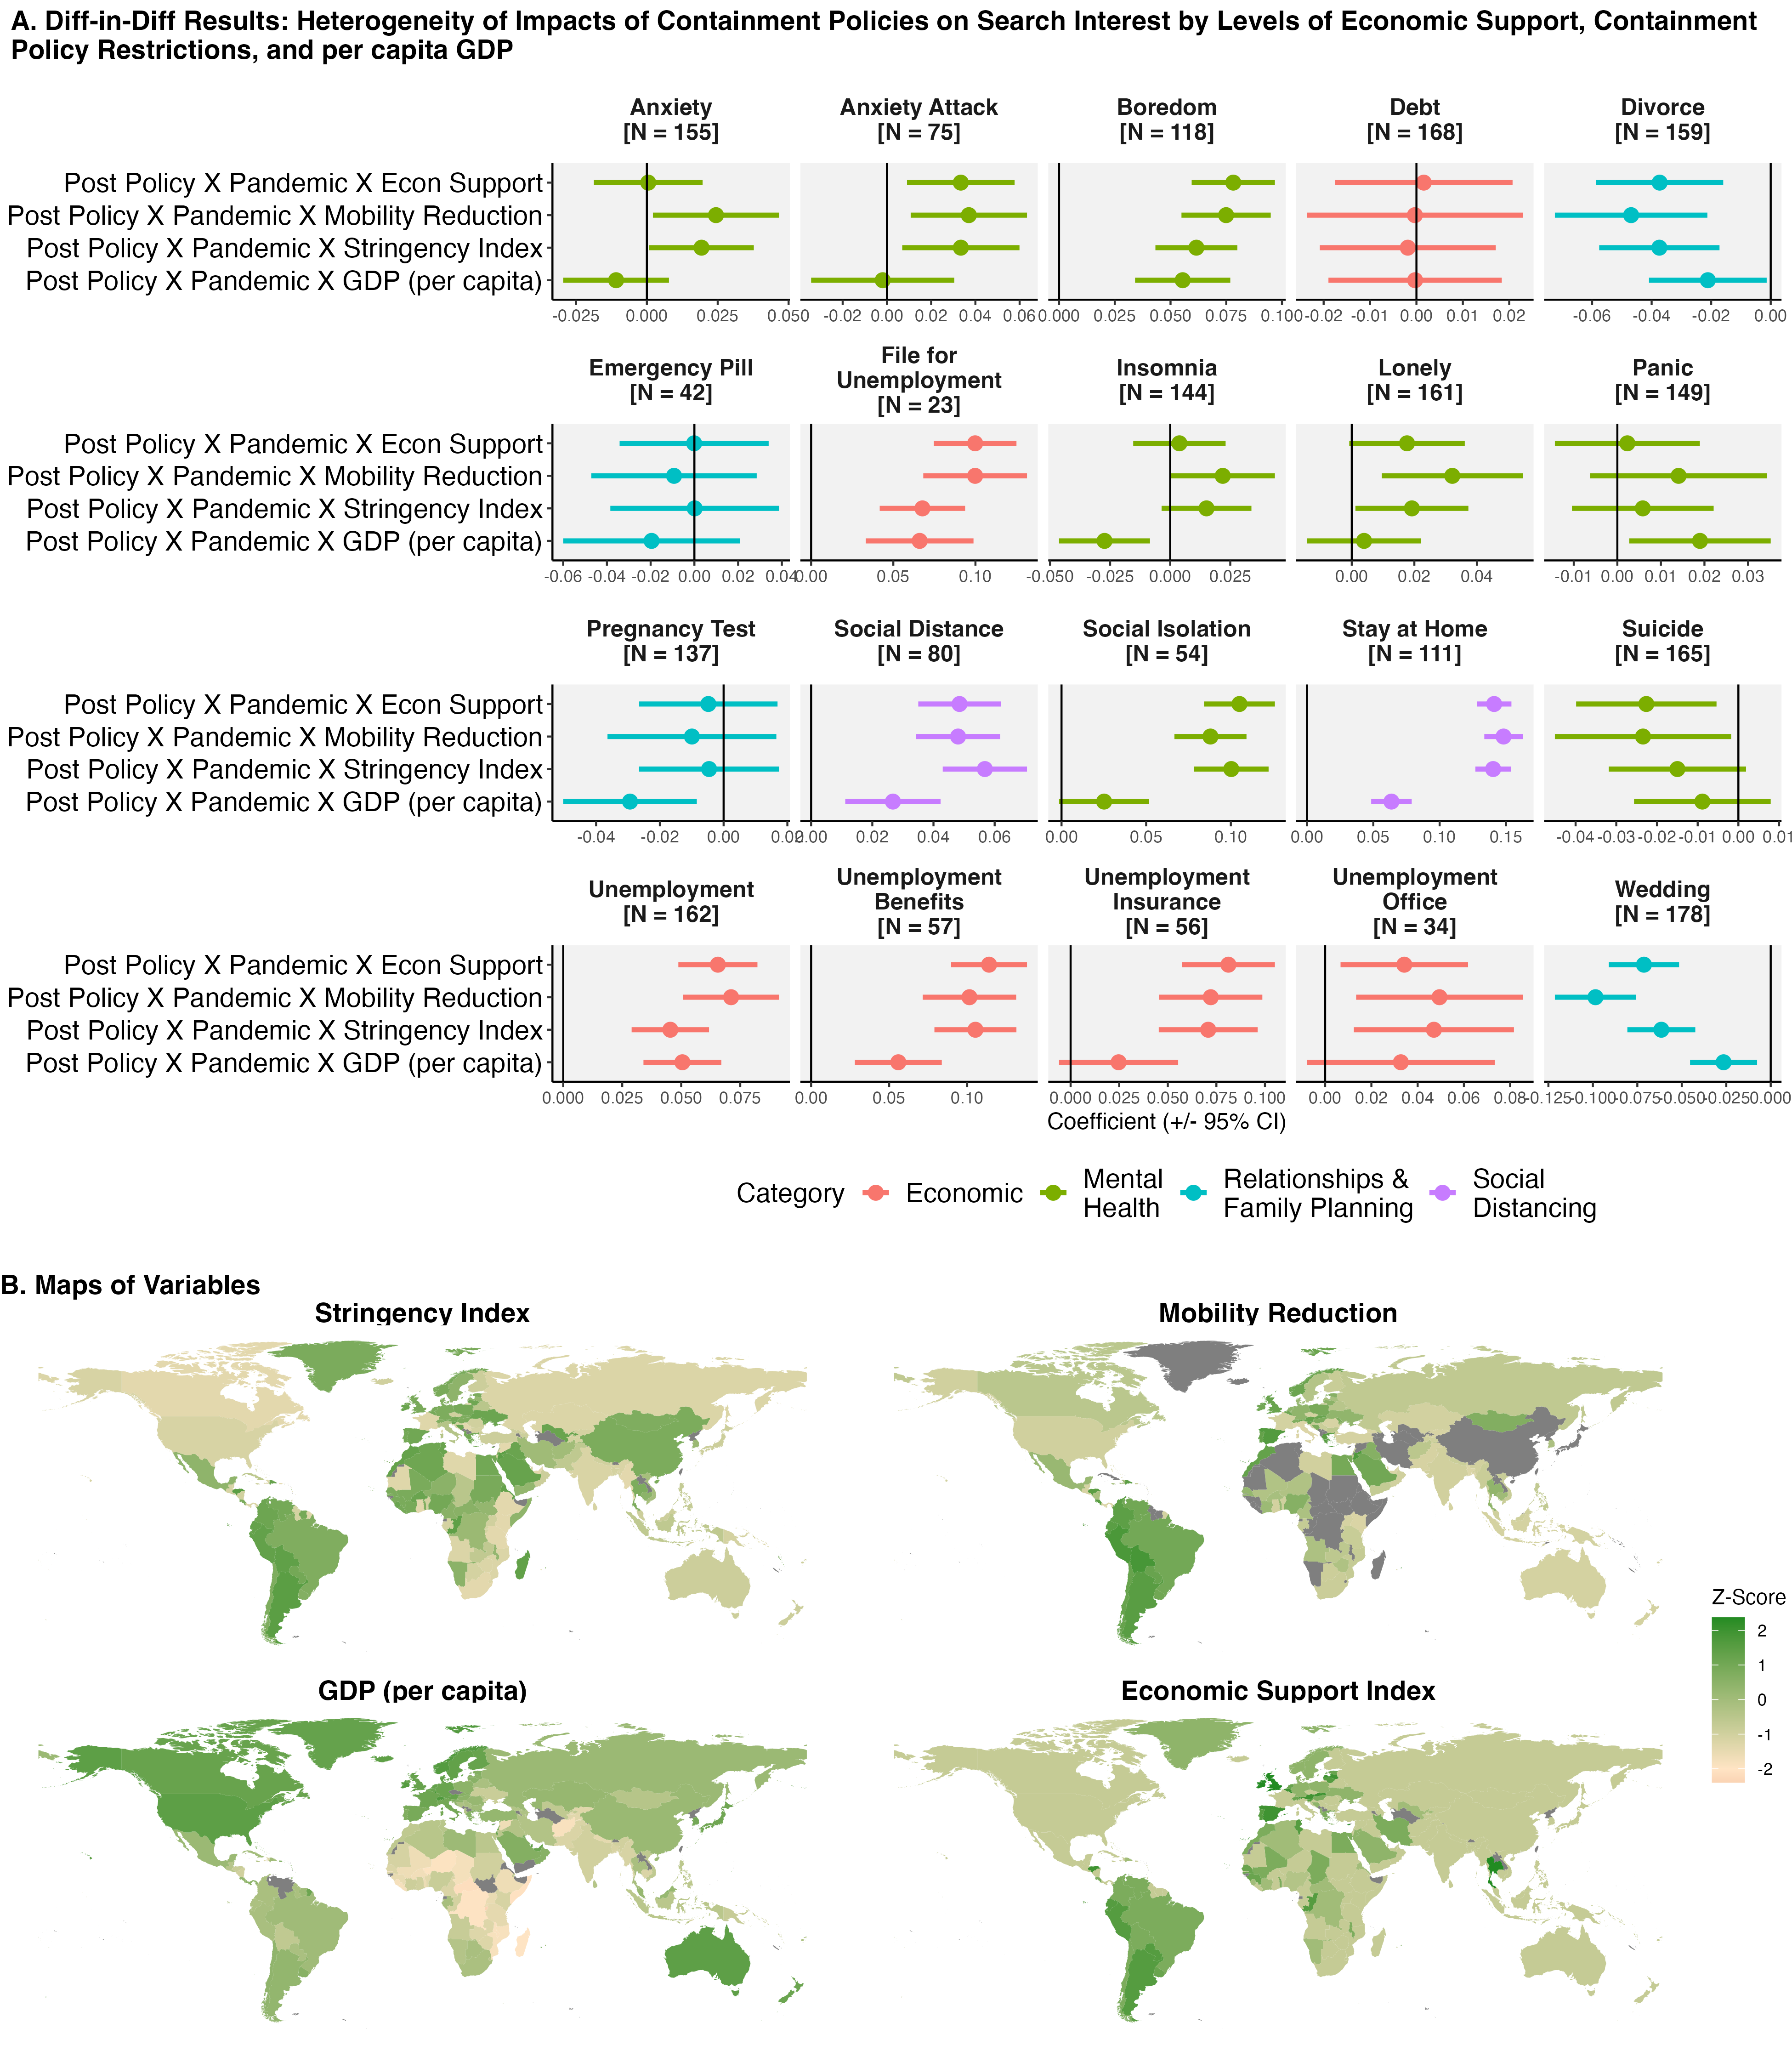
\includegraphics[width=0.85\textwidth]{figures/did_interact_map_30.png}
    \caption{Association of COVID-19 policies on search interest: difference-in-differences results that explore heterogeneity of results across containment policy restrictiveness, economic support, and GDP per capita. Each coefficient comes from a separate regression. The stringency index comes from the University of Oxford COVID-19 Government Response tracker, a composite measure of the restrictiveness of policy measures. Mobility reduction comes from Google COVID-19 Community Mobility Reports, which measure the percent change in mobility relative to pre-pandemic levels. Per capita GDP comes from the World Bank's World Development Indicators; we use log per capita GDP. The Economic Support index from the Oxford COVID-19 Government Response tracker, which measures the extent of economic support across metrics such as income support and debt relief. We standardize all variables into z-scores---having a mean of zero and standard deviation of one. `N' indicates the number of countries with available data. Maps produced using R, version 4.2.2 (\url{https://www.r-project.org/}); data for country boundaries come from Natural Earth (\url{https://www.naturalearthdata.com/}).}
    \label{fig:did_interact_map_30}
\end{figure}

\begin{figure}[H]
    \centering
    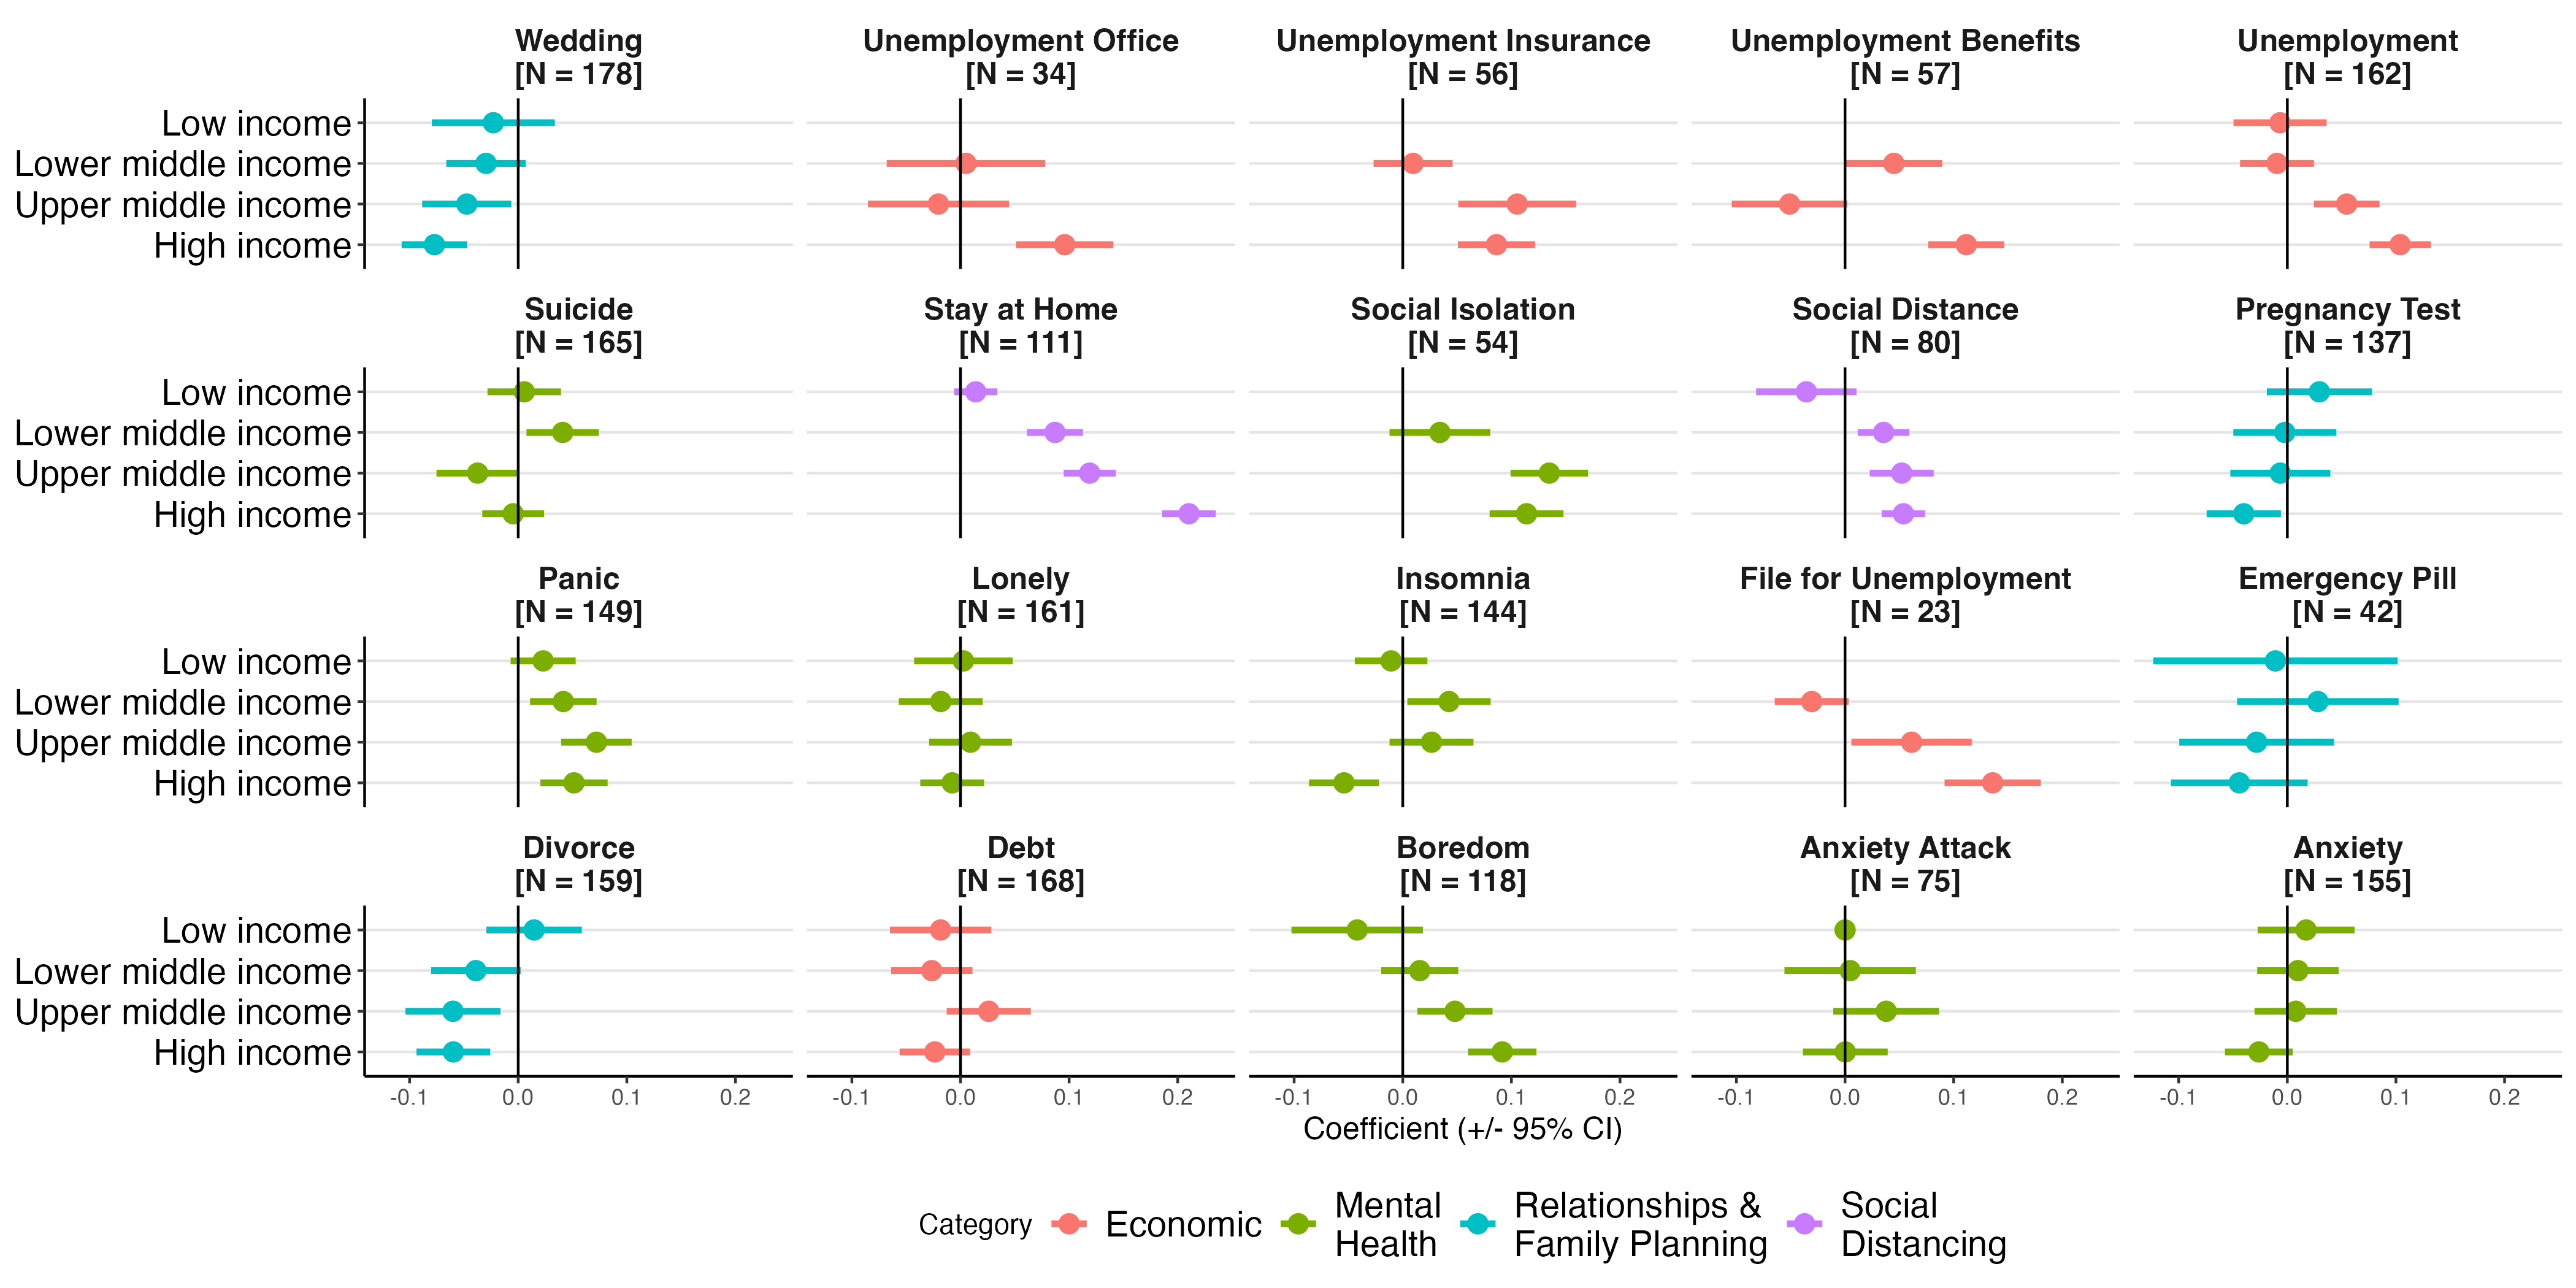
\includegraphics[width=0.85\textwidth]{figures/did_income_30.png}
    \caption{Association of COVID-19 policies with search interest: difference-in-difference results pooling countries by income level. Point estimates and 95\% confidence intervals are shown. `N' indicates the number of countries with available data.}
    \label{fig:did_income_30}
\end{figure}

% --------------------------
\newpage
\subsection{60 day threshold}

\begin{figure}[H]
    \centering
    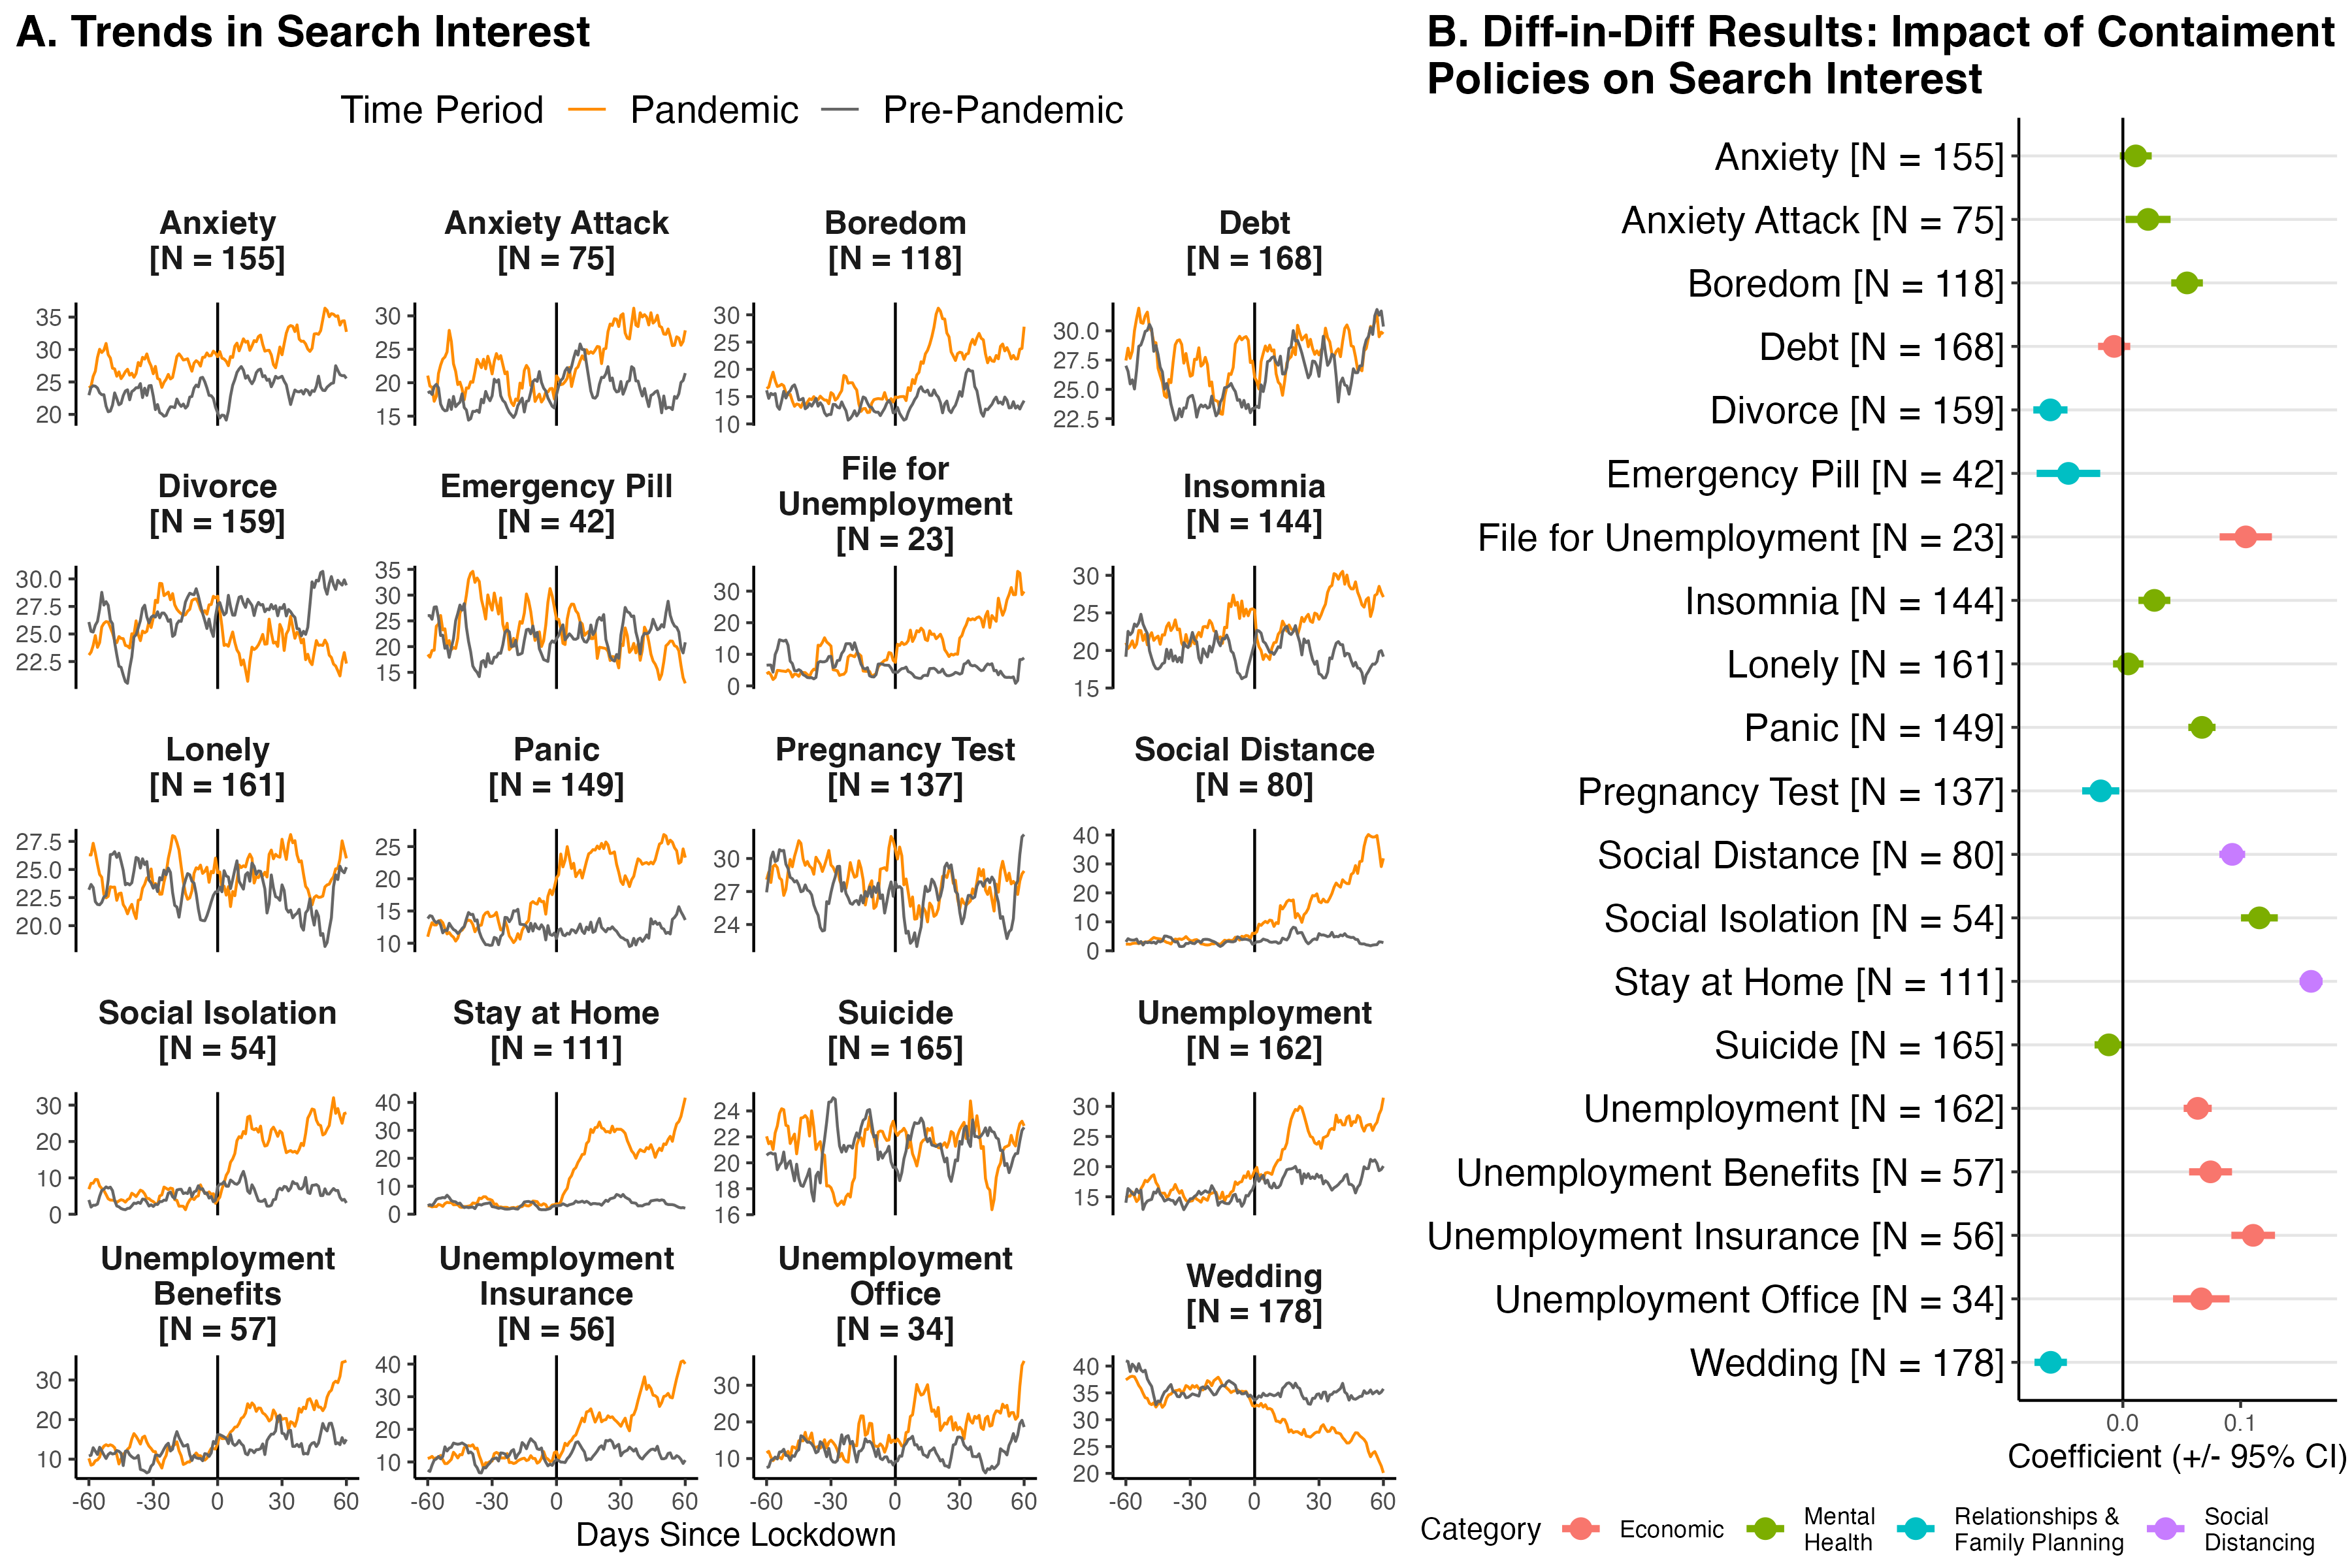
\includegraphics[width=0.85\textwidth]{figures/did_overall_60.png}
    \caption{Association of COVID-19 policies with search interest: results pooling all countries. Point estimates and 95\% confidence intervals are shown. To more clearly show trends, the seven day moving average of search interest is shown in panel A. `N' indicates the number of countries with available data.}
    \label{fig:lockdown_impact_60}
\end{figure}

\begin{figure}[H]
    \centering
    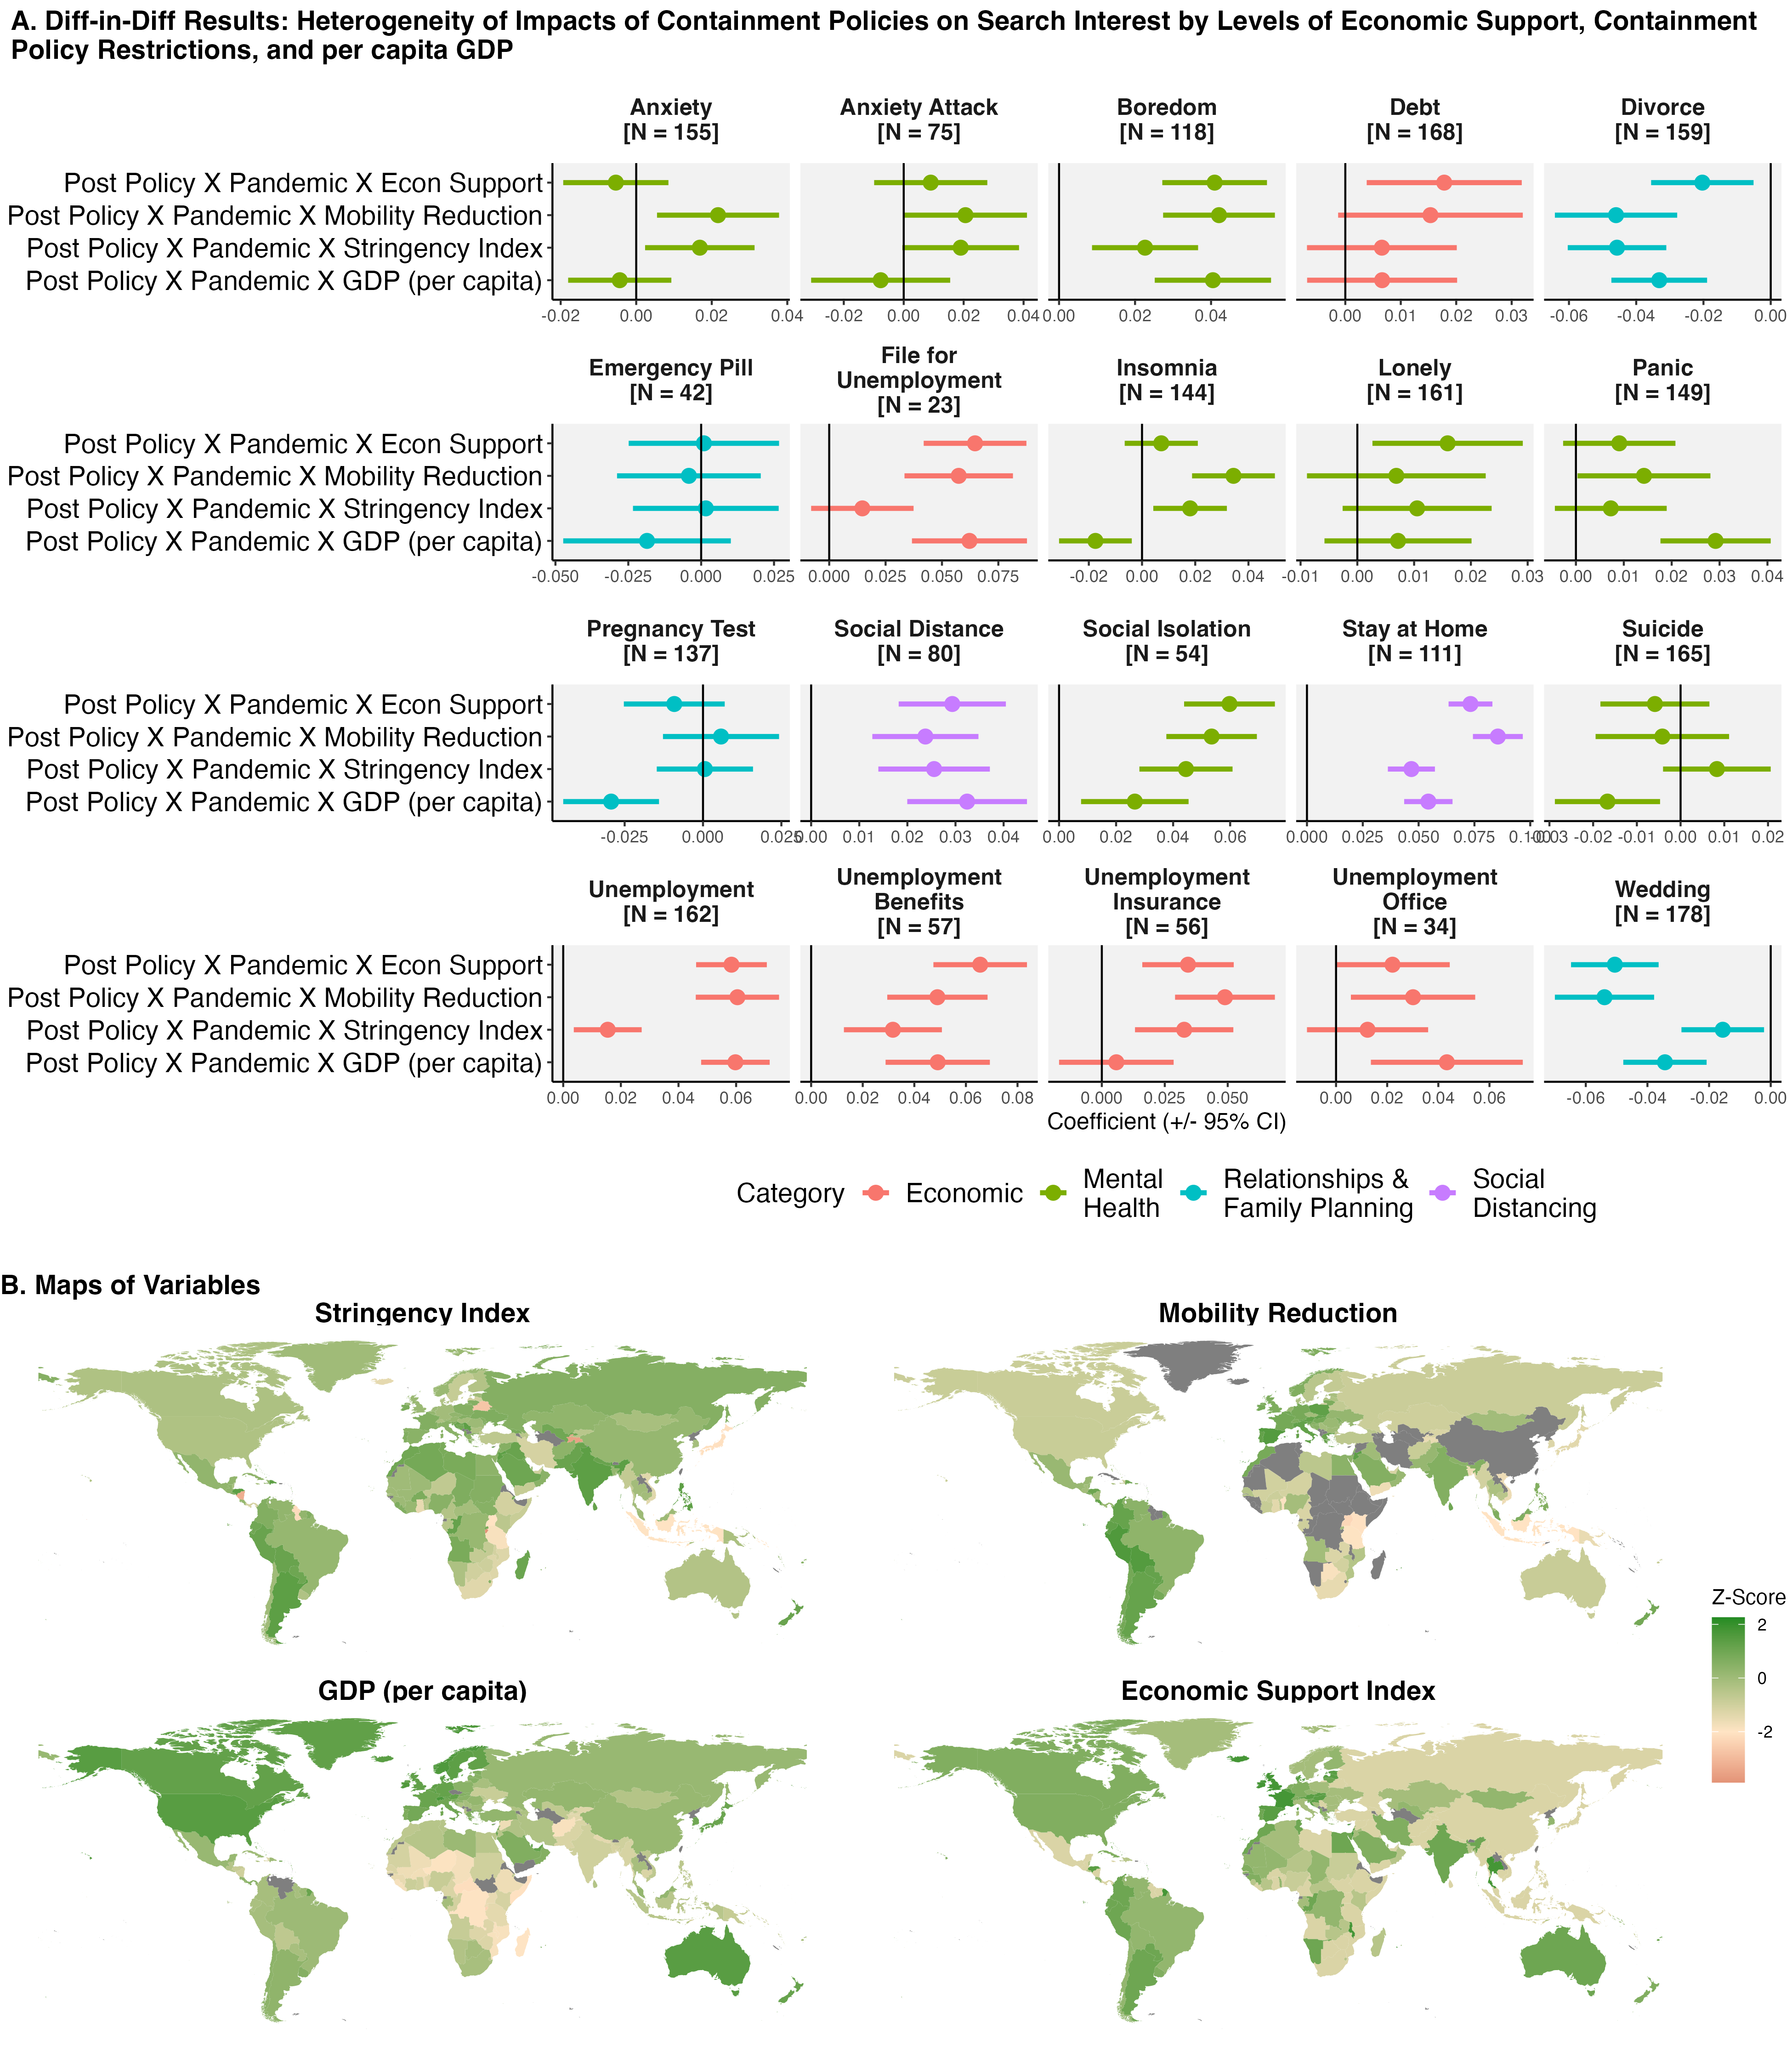
\includegraphics[width=0.85\textwidth]{figures/did_interact_map_60.png}
    \caption{Association of COVID-19 policies with search interest: difference-in-differences results that explore heterogeneity of results across containment policy restrictiveness, economic support, and GDP per capita. Each coefficient comes from a separate regression. The stringency index comes from the University of Oxford COVID-19 Government Response tracker, a composite measure of the restrictiveness of policy measures. Mobility reduction comes from Google COVID-19 Community Mobility Reports, which measure the percent change in mobility relative to pre-pandemic levels. Per capita GDP comes from the World Bank's World Development Indicators; we use log per capita GDP. The Economic Support index from the Oxford COVID-19 Government Response tracker, which measures the extent of economic support across metrics such as income support and debt relief. We standardize all variables into z-scores---having a mean of zero and standard deviation of one. `N' indicates the number of countries with available data. Maps produced using R, version 4.2.2 (\url{https://www.r-project.org/}); data for country boundaries come from Natural Earth (\url{https://www.naturalearthdata.com/}).}
    \label{fig:did_interact_map_60}
\end{figure}

\begin{figure}[H]
    \centering
    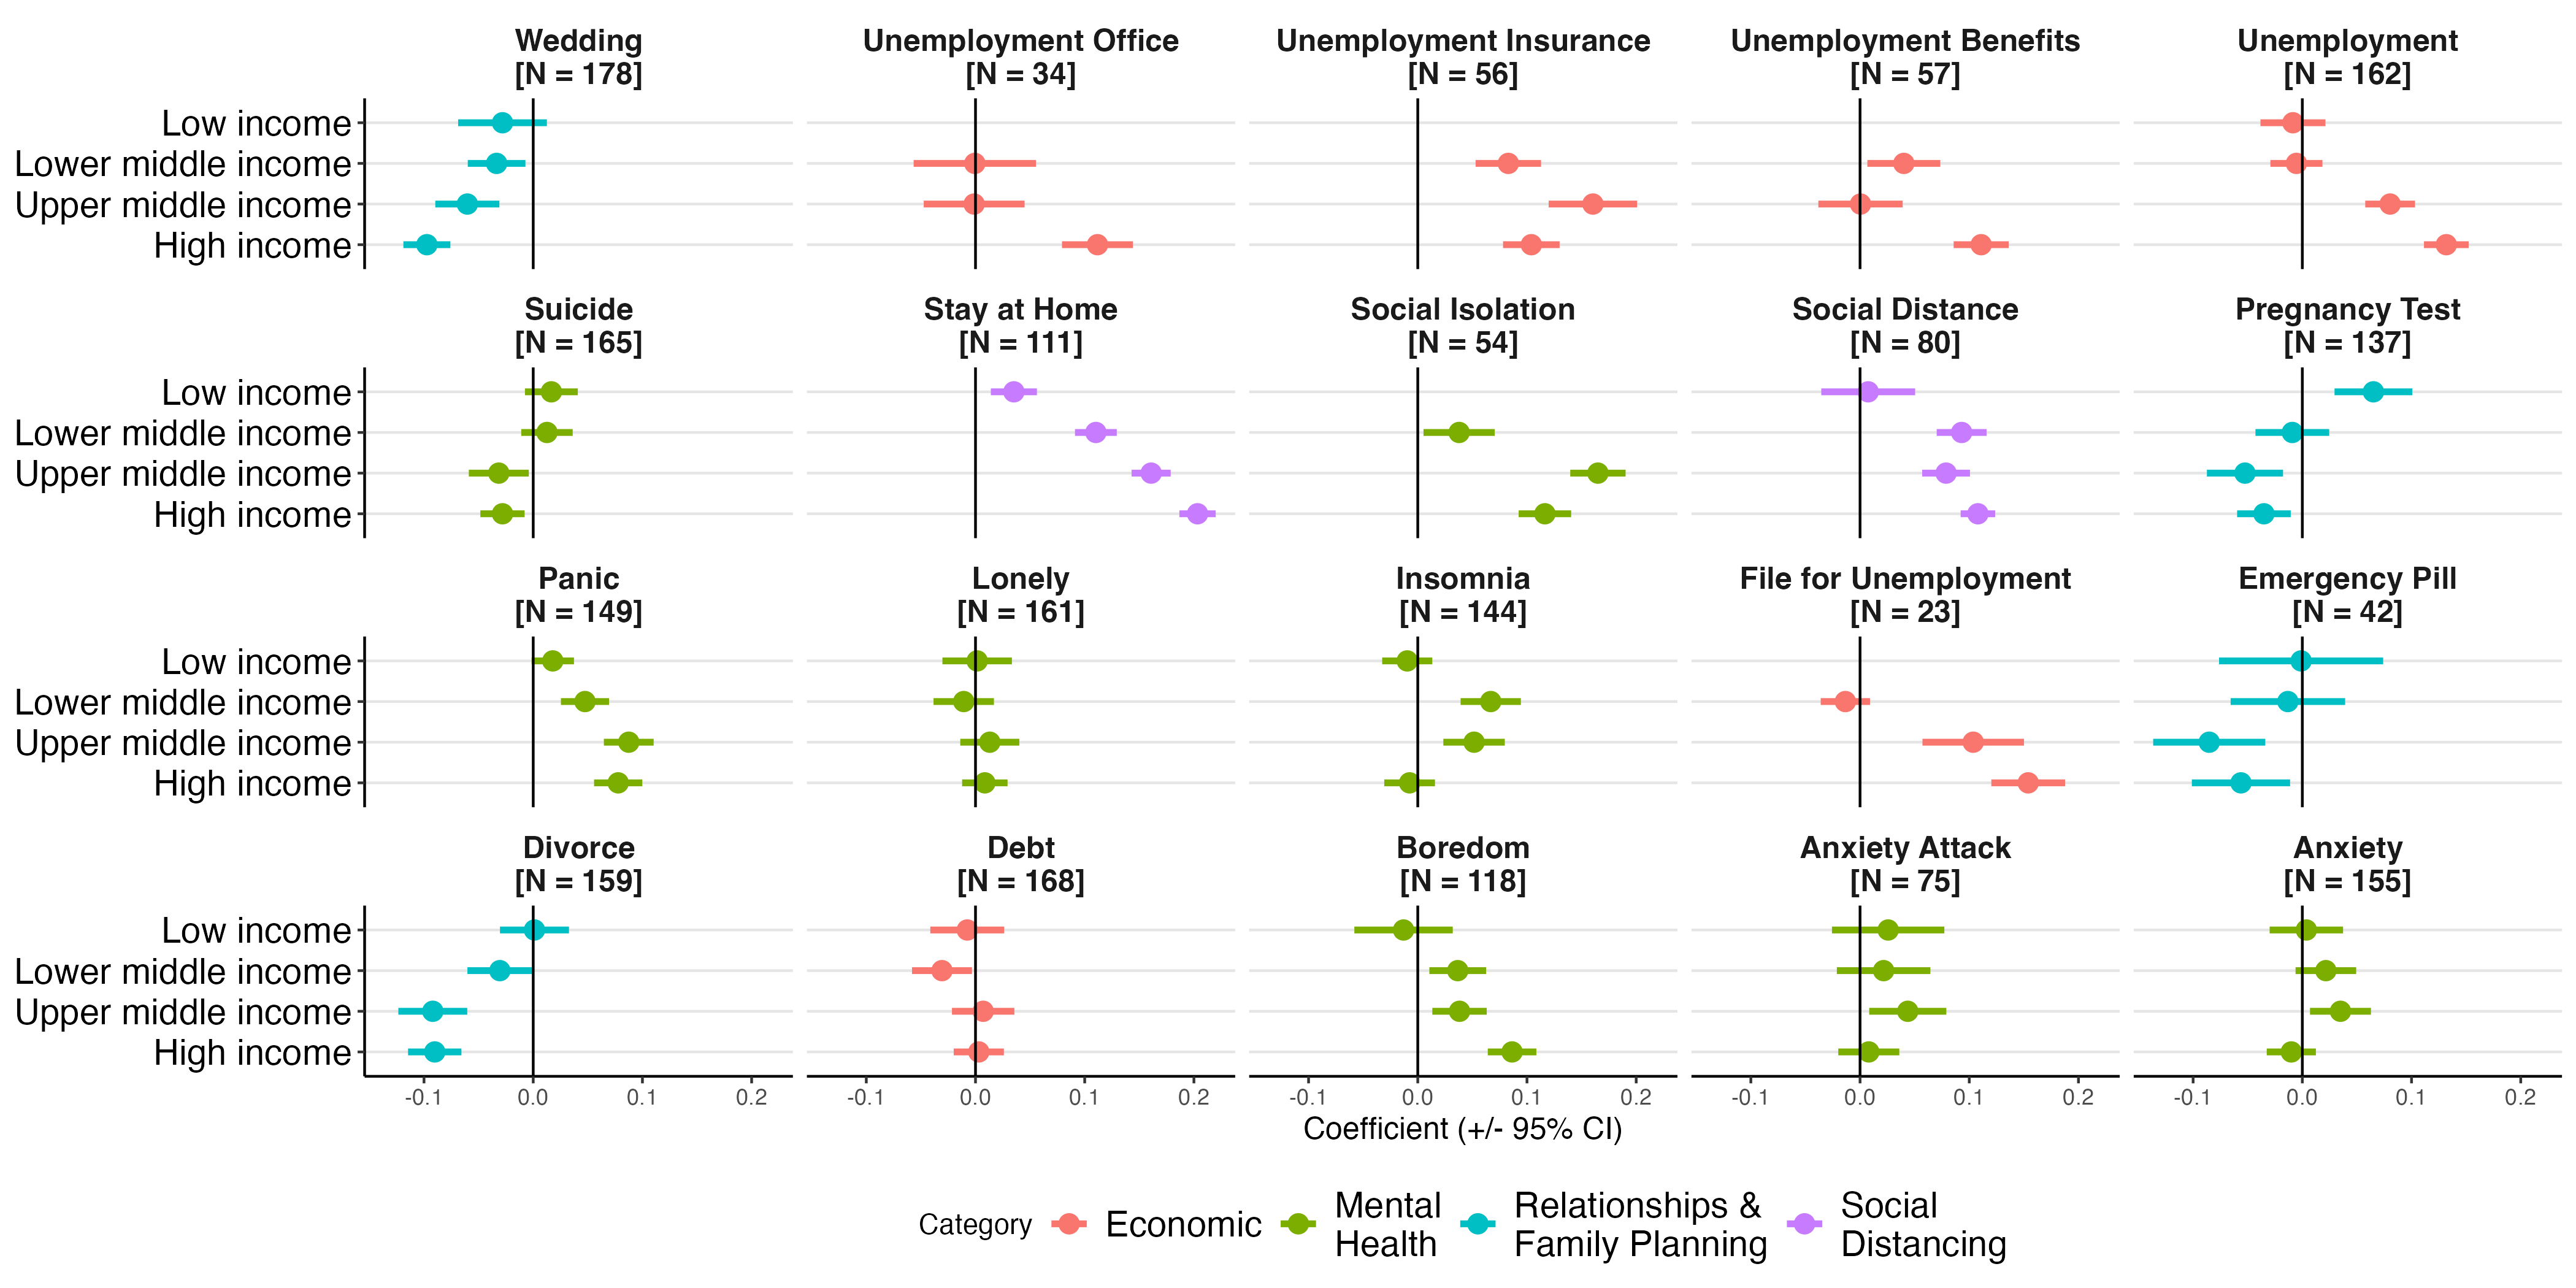
\includegraphics[width=0.85\textwidth]{figures/did_income_60.png}
    \caption{Association of COVID-19 policies with search interest: difference-in-difference results pooling countries by income level. Point estimates and 95\% confidence intervals are shown. `N' indicates the number of countries with available data.}
    \label{fig:did_income_60}
\end{figure}

% --------------------------
\newpage
\subsection{120 day threshold}

\begin{figure}[H]
    \centering
    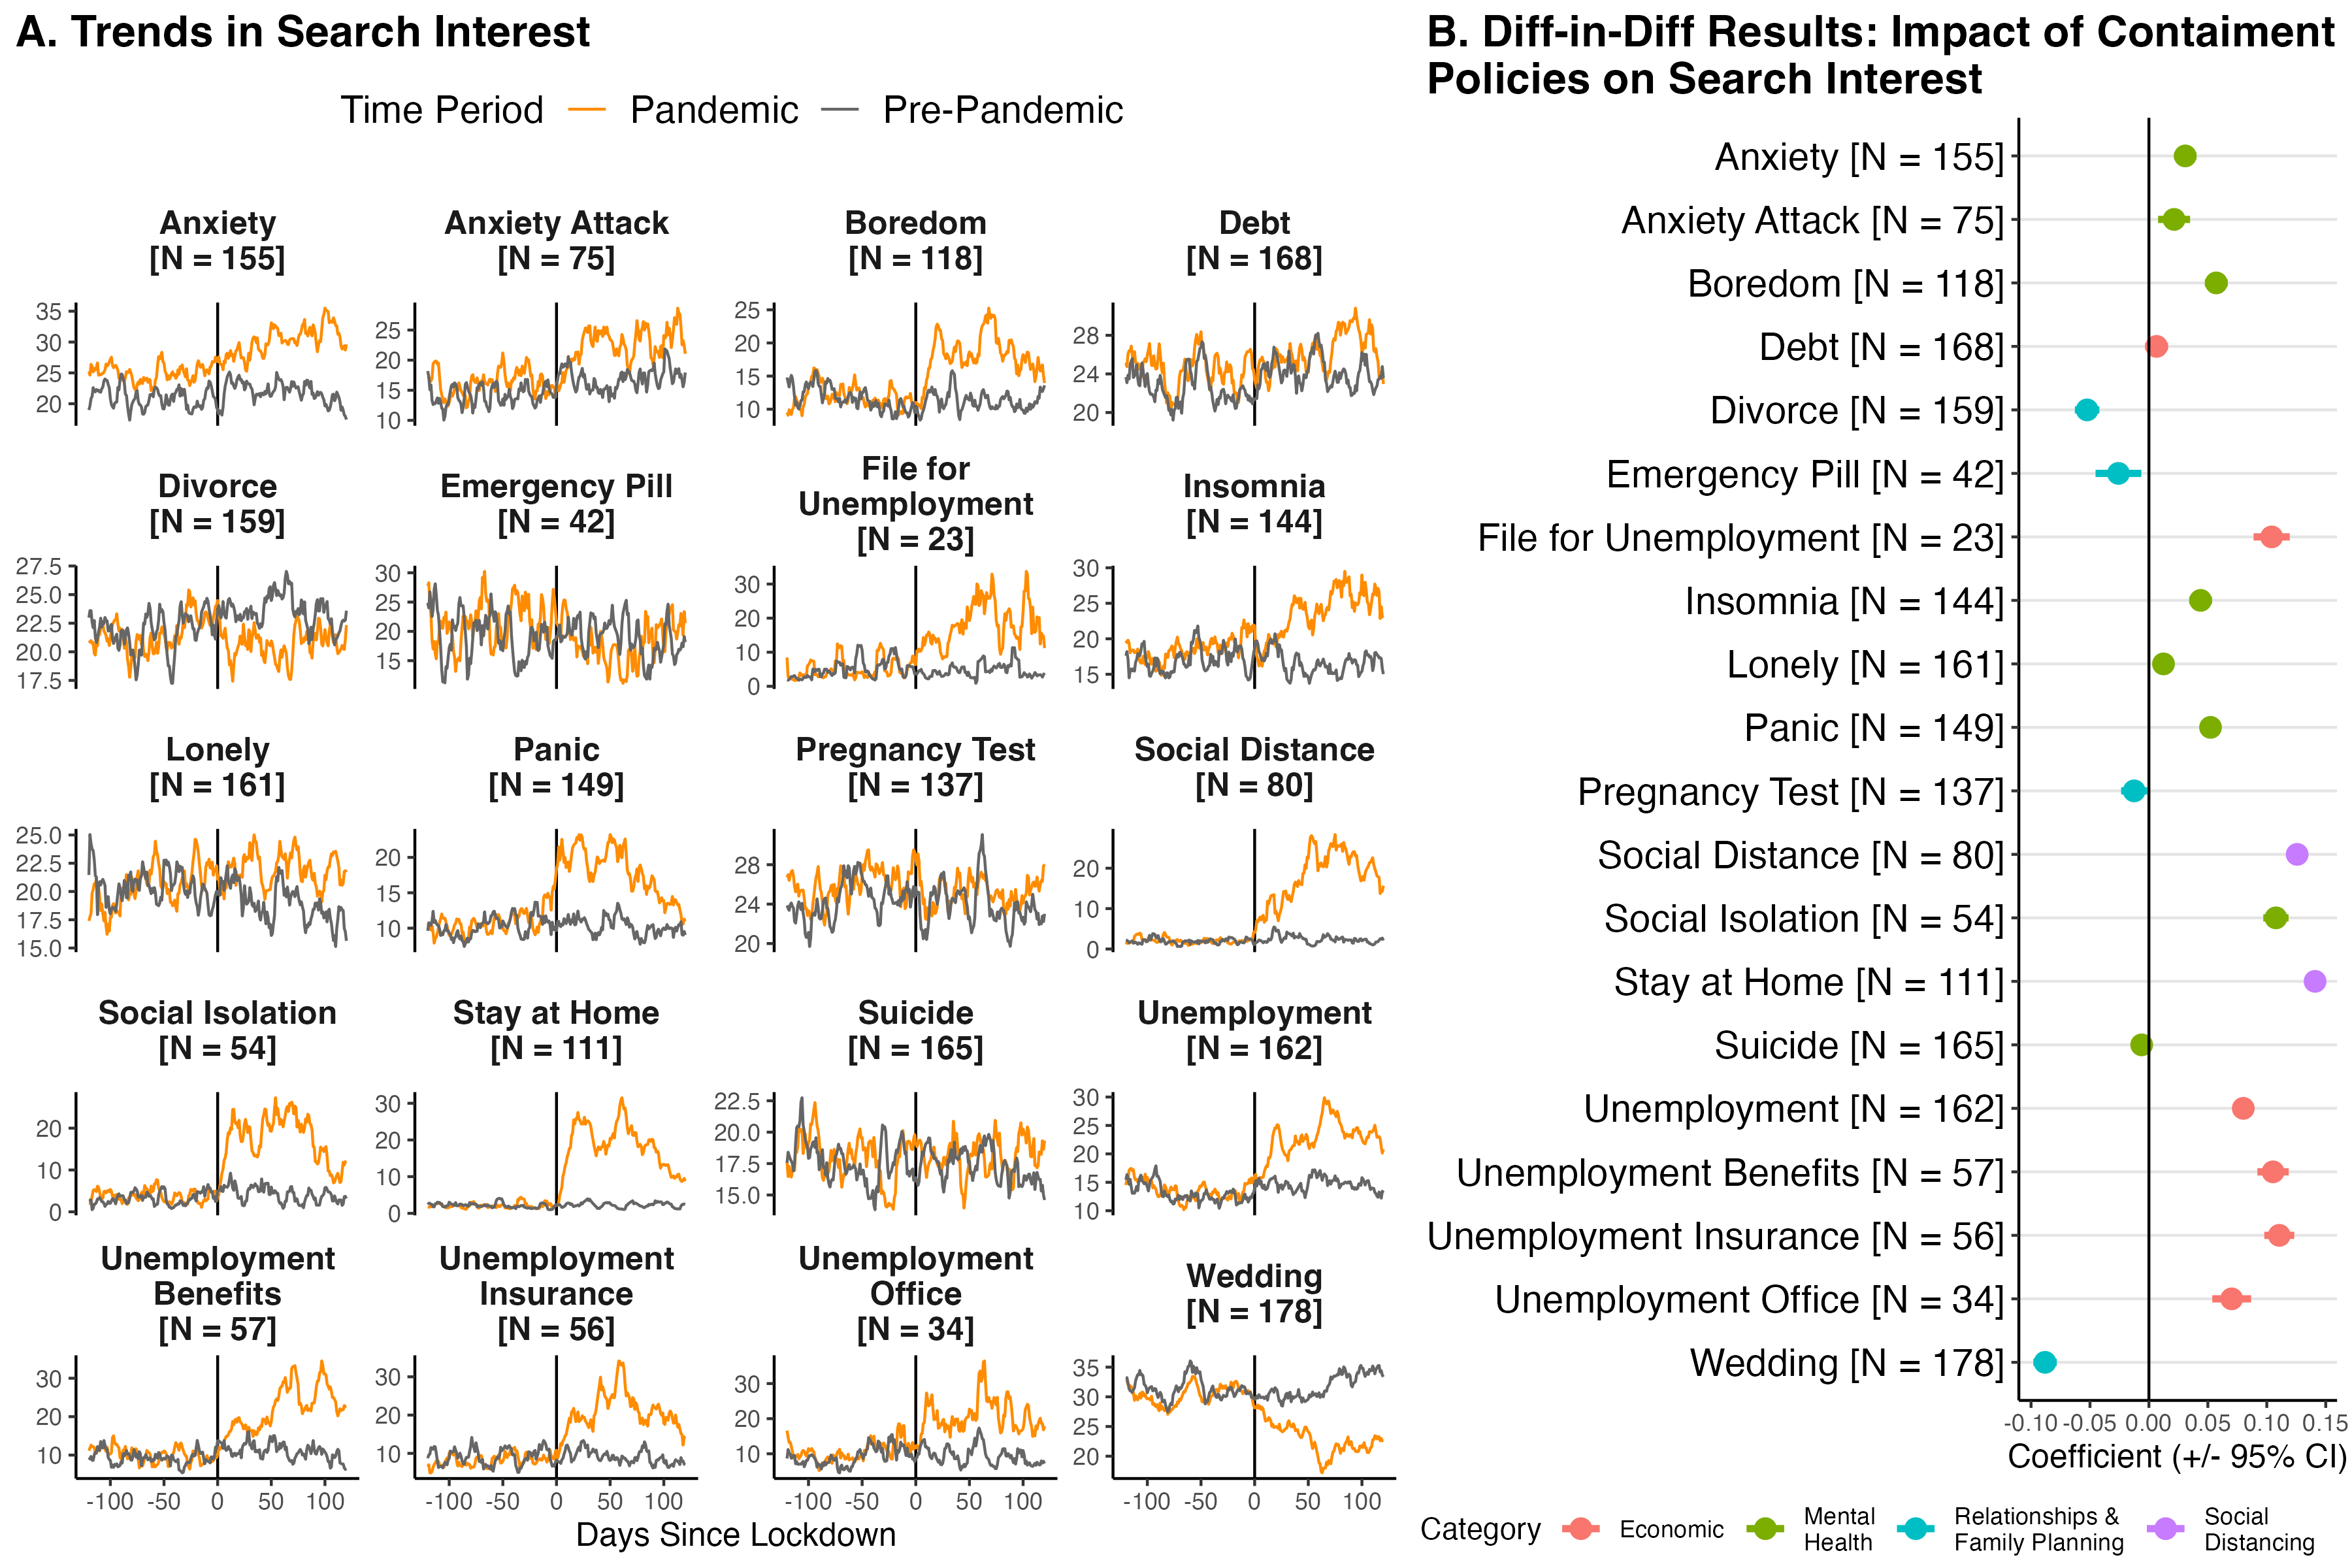
\includegraphics[width=0.85\textwidth]{figures/did_overall_120.png}
    \caption{Association of COVID-19 policies with search interest: results pooling all countries. Point estimates and 95\% confidence intervals are shown. To more clearly show trends, the seven day moving average of search interest is shown in panel A. `N' indicates the number of countries with available data.}
    \label{fig:lockdown_impact_120}
\end{figure}

\begin{figure}[H]
    \centering
    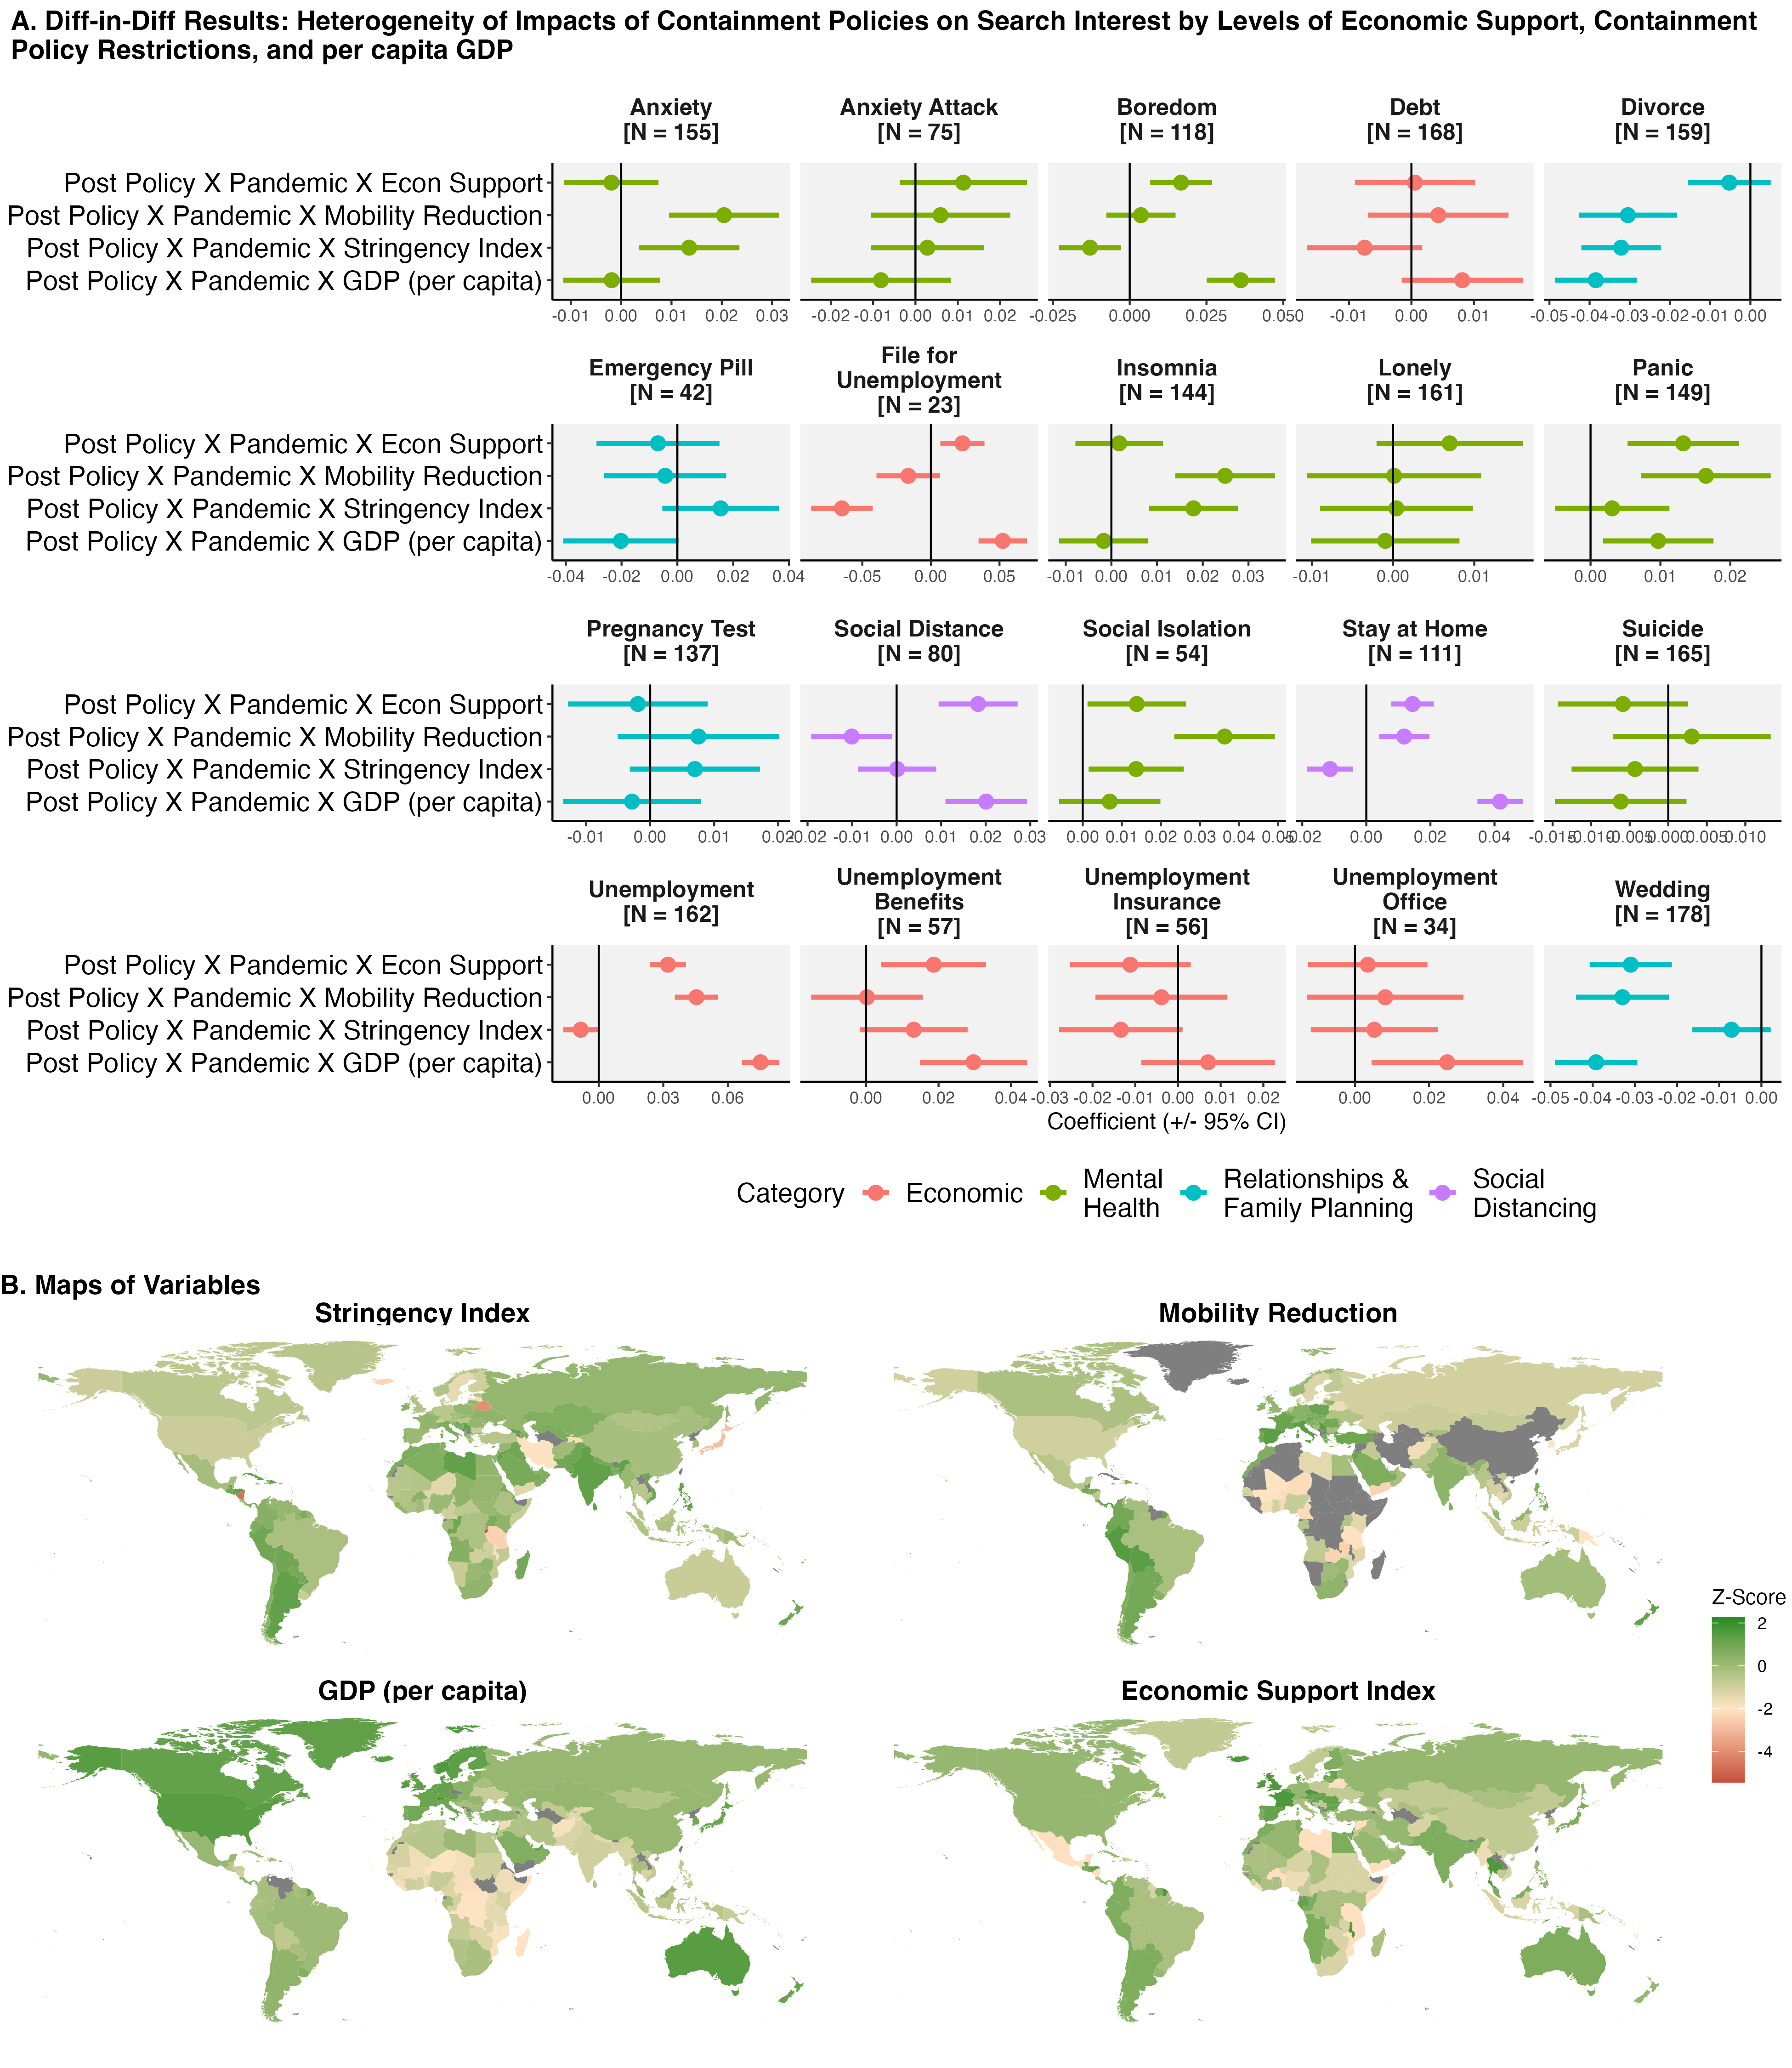
\includegraphics[width=0.85\textwidth]{figures/did_interact_map_120.png}
    \caption{Association of COVID-19 policies with search interest: difference-in-differences results that explore heterogeneity of results across containment policy restrictiveness, economic support, and GDP per capita. Each coefficient comes from a separate regression. The stringency index comes from the University of Oxford COVID-19 Government Response tracker, a composite measure of the restrictiveness of policy measures. Mobility reduction comes from Google COVID-19 Community Mobility Reports, which measure the percent change in mobility relative to pre-pandemic levels. Per capita GDP comes from the World Bank's World Development Indicators; we use log per capita GDP. The Economic Support index from the Oxford COVID-19 Government Response tracker, which measures the extent of economic support across metrics such as income support and debt relief. We standardize all variables into z-scores---having a mean of zero and standard deviation of one. `N' indicates the number of countries with available data. Maps produced using R, version 4.2.2 (\url{https://www.r-project.org/}); data for country boundaries come from Natural Earth (\url{https://www.naturalearthdata.com/}).}
    \label{fig:did_interact_map_120}
\end{figure}

\begin{figure}[H]
    \centering
    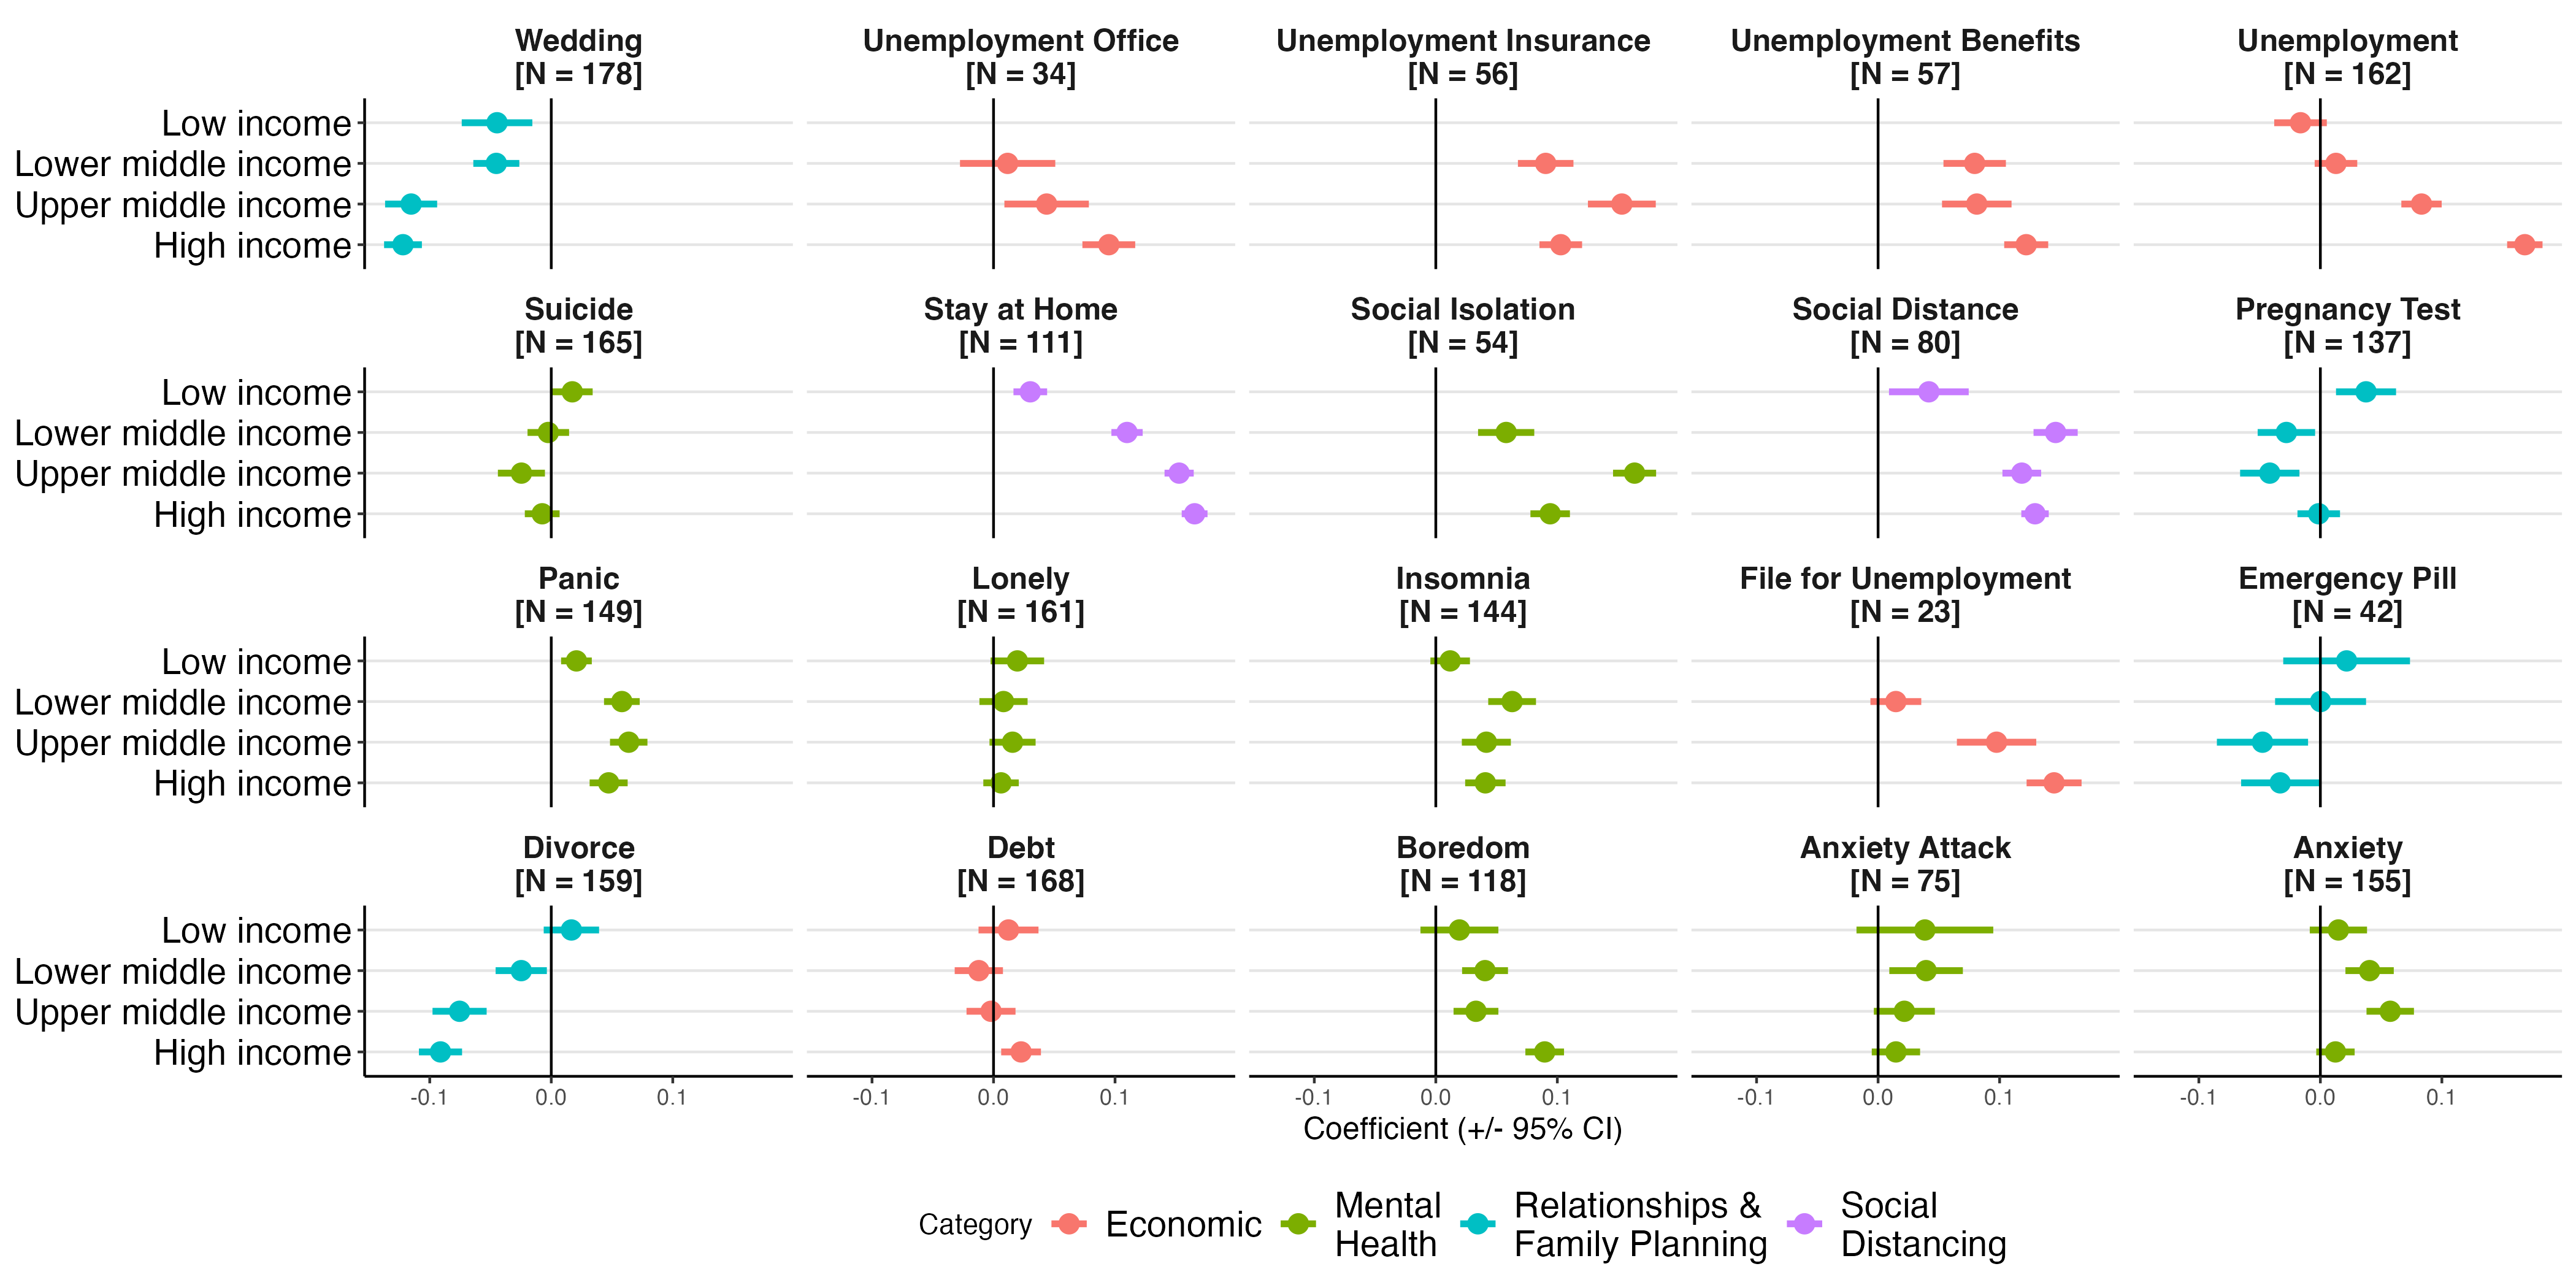
\includegraphics[width=0.85\textwidth]{figures/did_income_120.png}
    \caption{Association of COVID-19 policies with search interest: difference-in-difference results pooling countries by income level. Point estimates and 95\% confidence intervals are shown. `N' indicates the number of countries with available data.}
    \label{fig:did_income_120}
\end{figure}

% --------------------------
\newpage
\subsection{180 day threshold}

\begin{figure}[H]
    \centering
    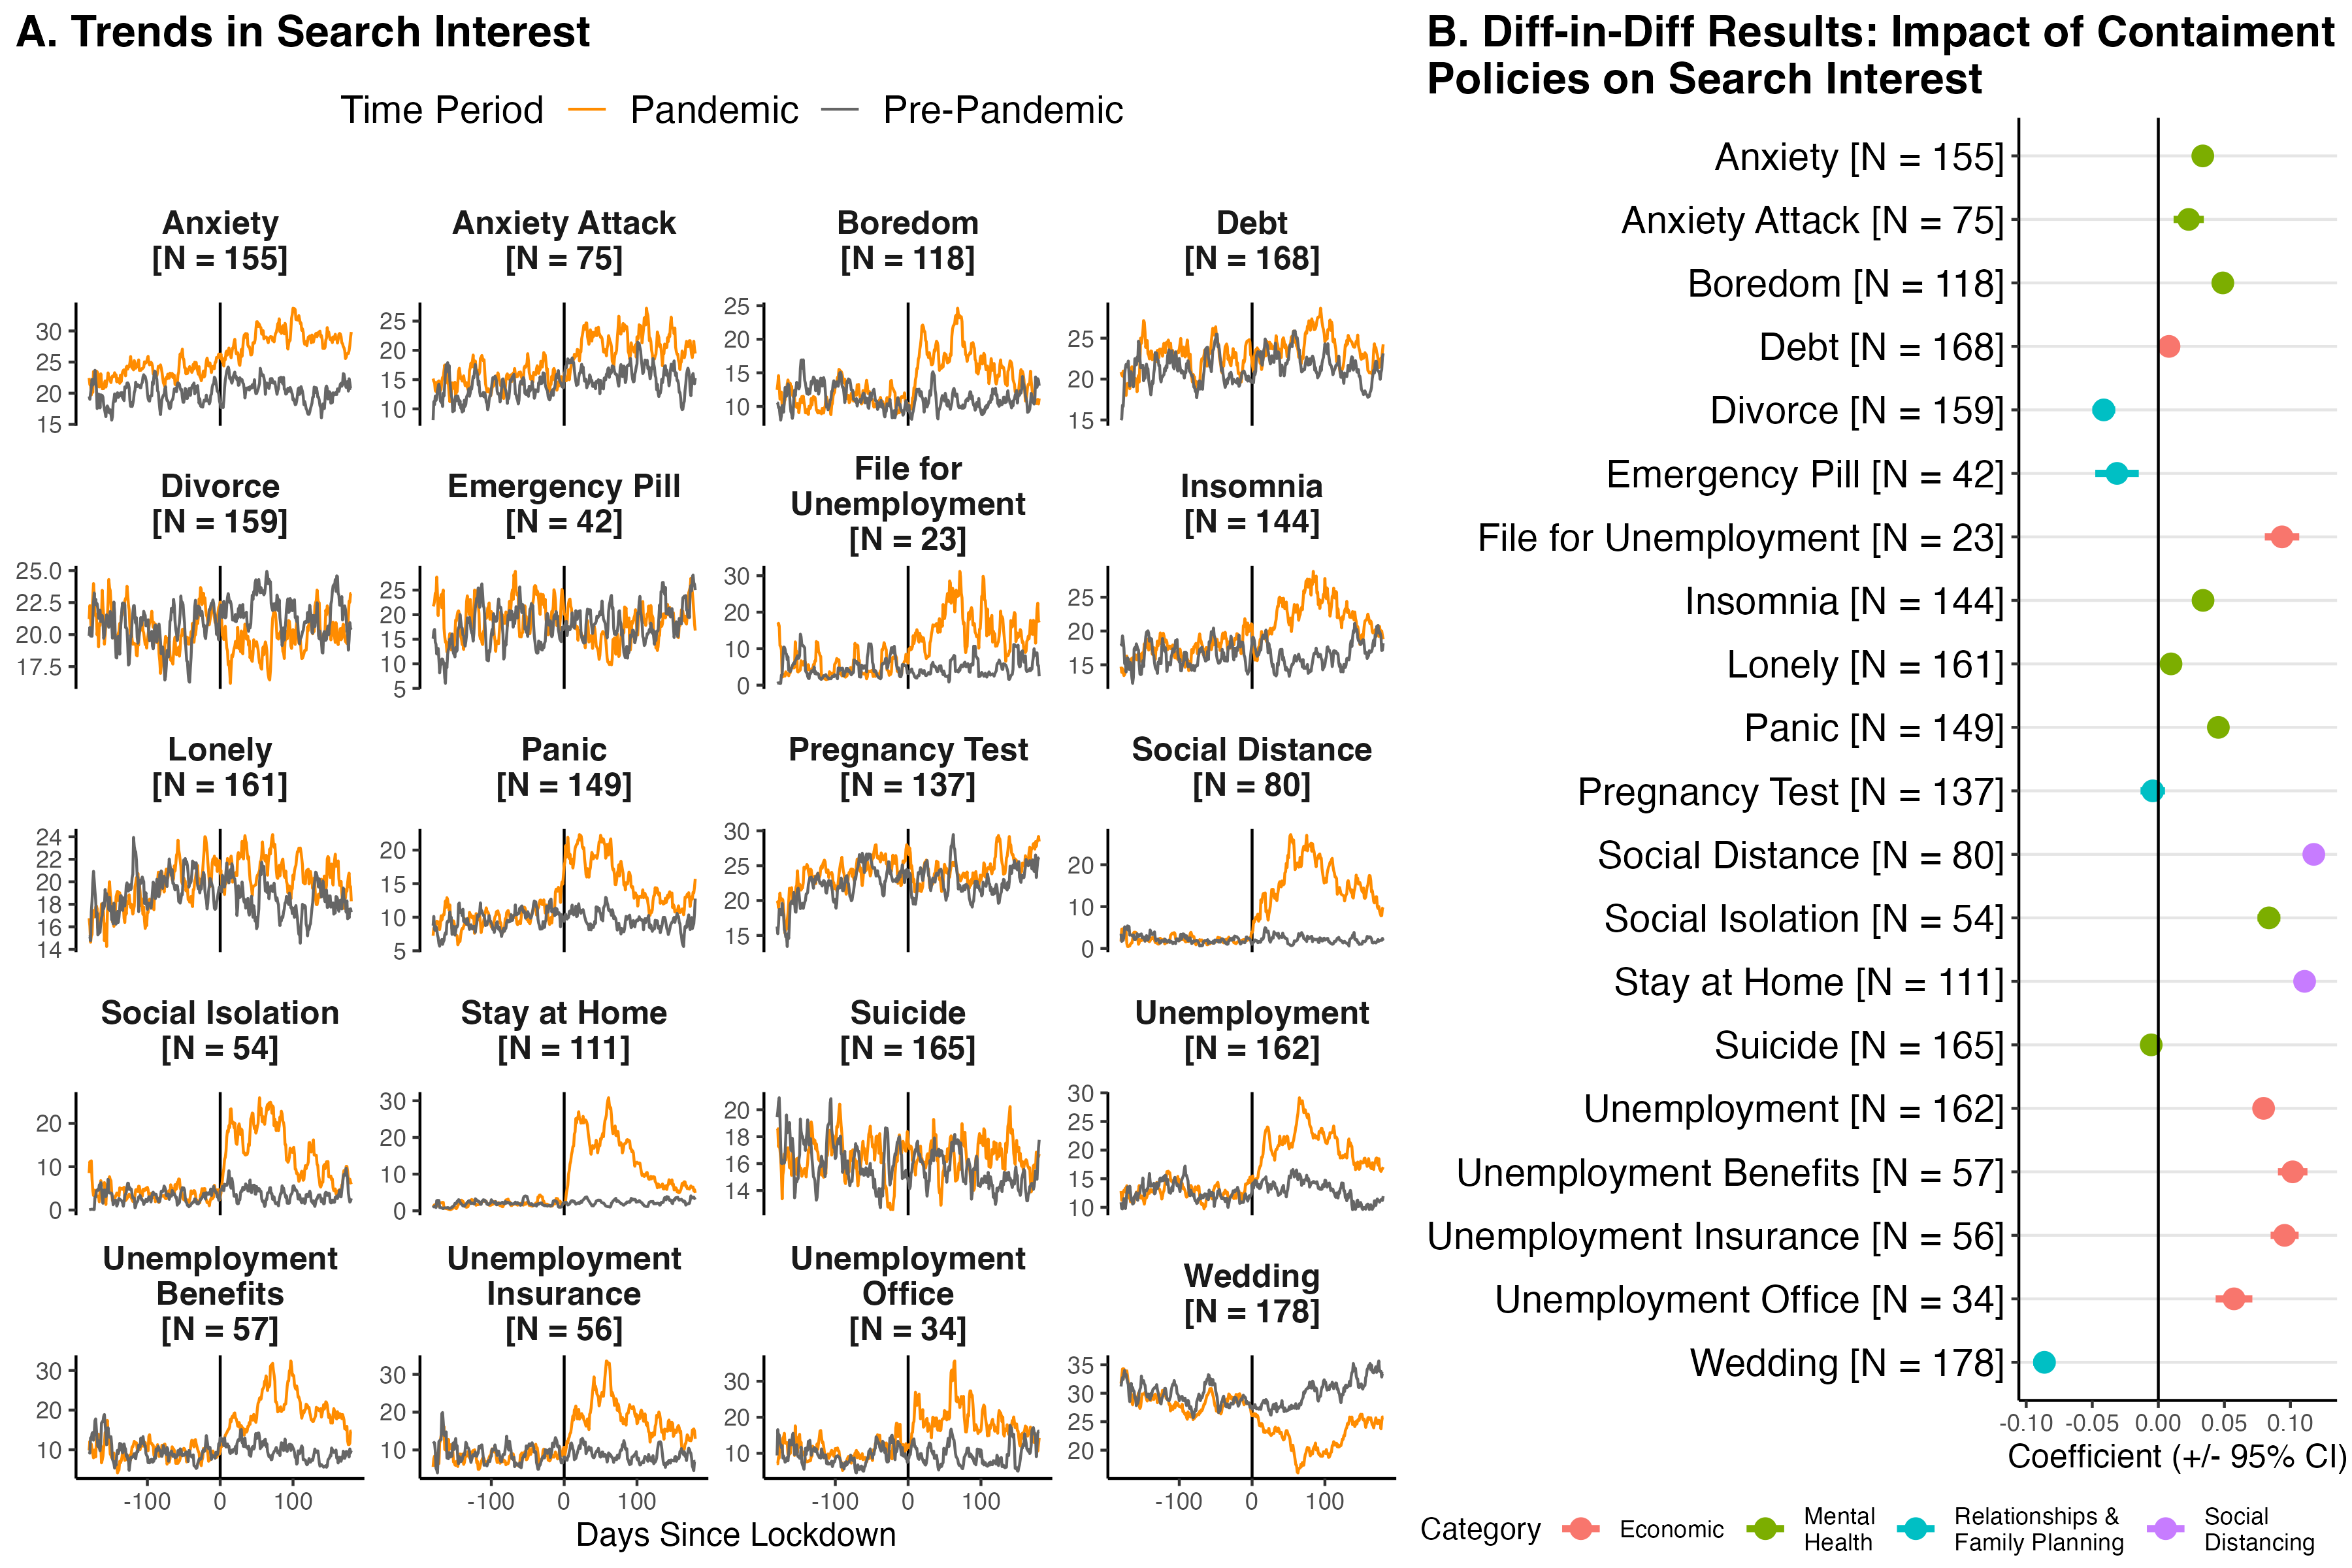
\includegraphics[width=0.85\textwidth]{figures/did_overall_180.png}
    \caption{\textcolor{black}{Association of COVID-19 policies with search interest: results pooling all countries. Point estimates and 95\% confidence intervals are shown. To more clearly show trends, the seven day moving average of search interest is shown in panel A. `N' indicates the number of countries with available data.}}
    \label{fig:lockdown_impact_180}
\end{figure}

\begin{figure}[H]
    \centering
    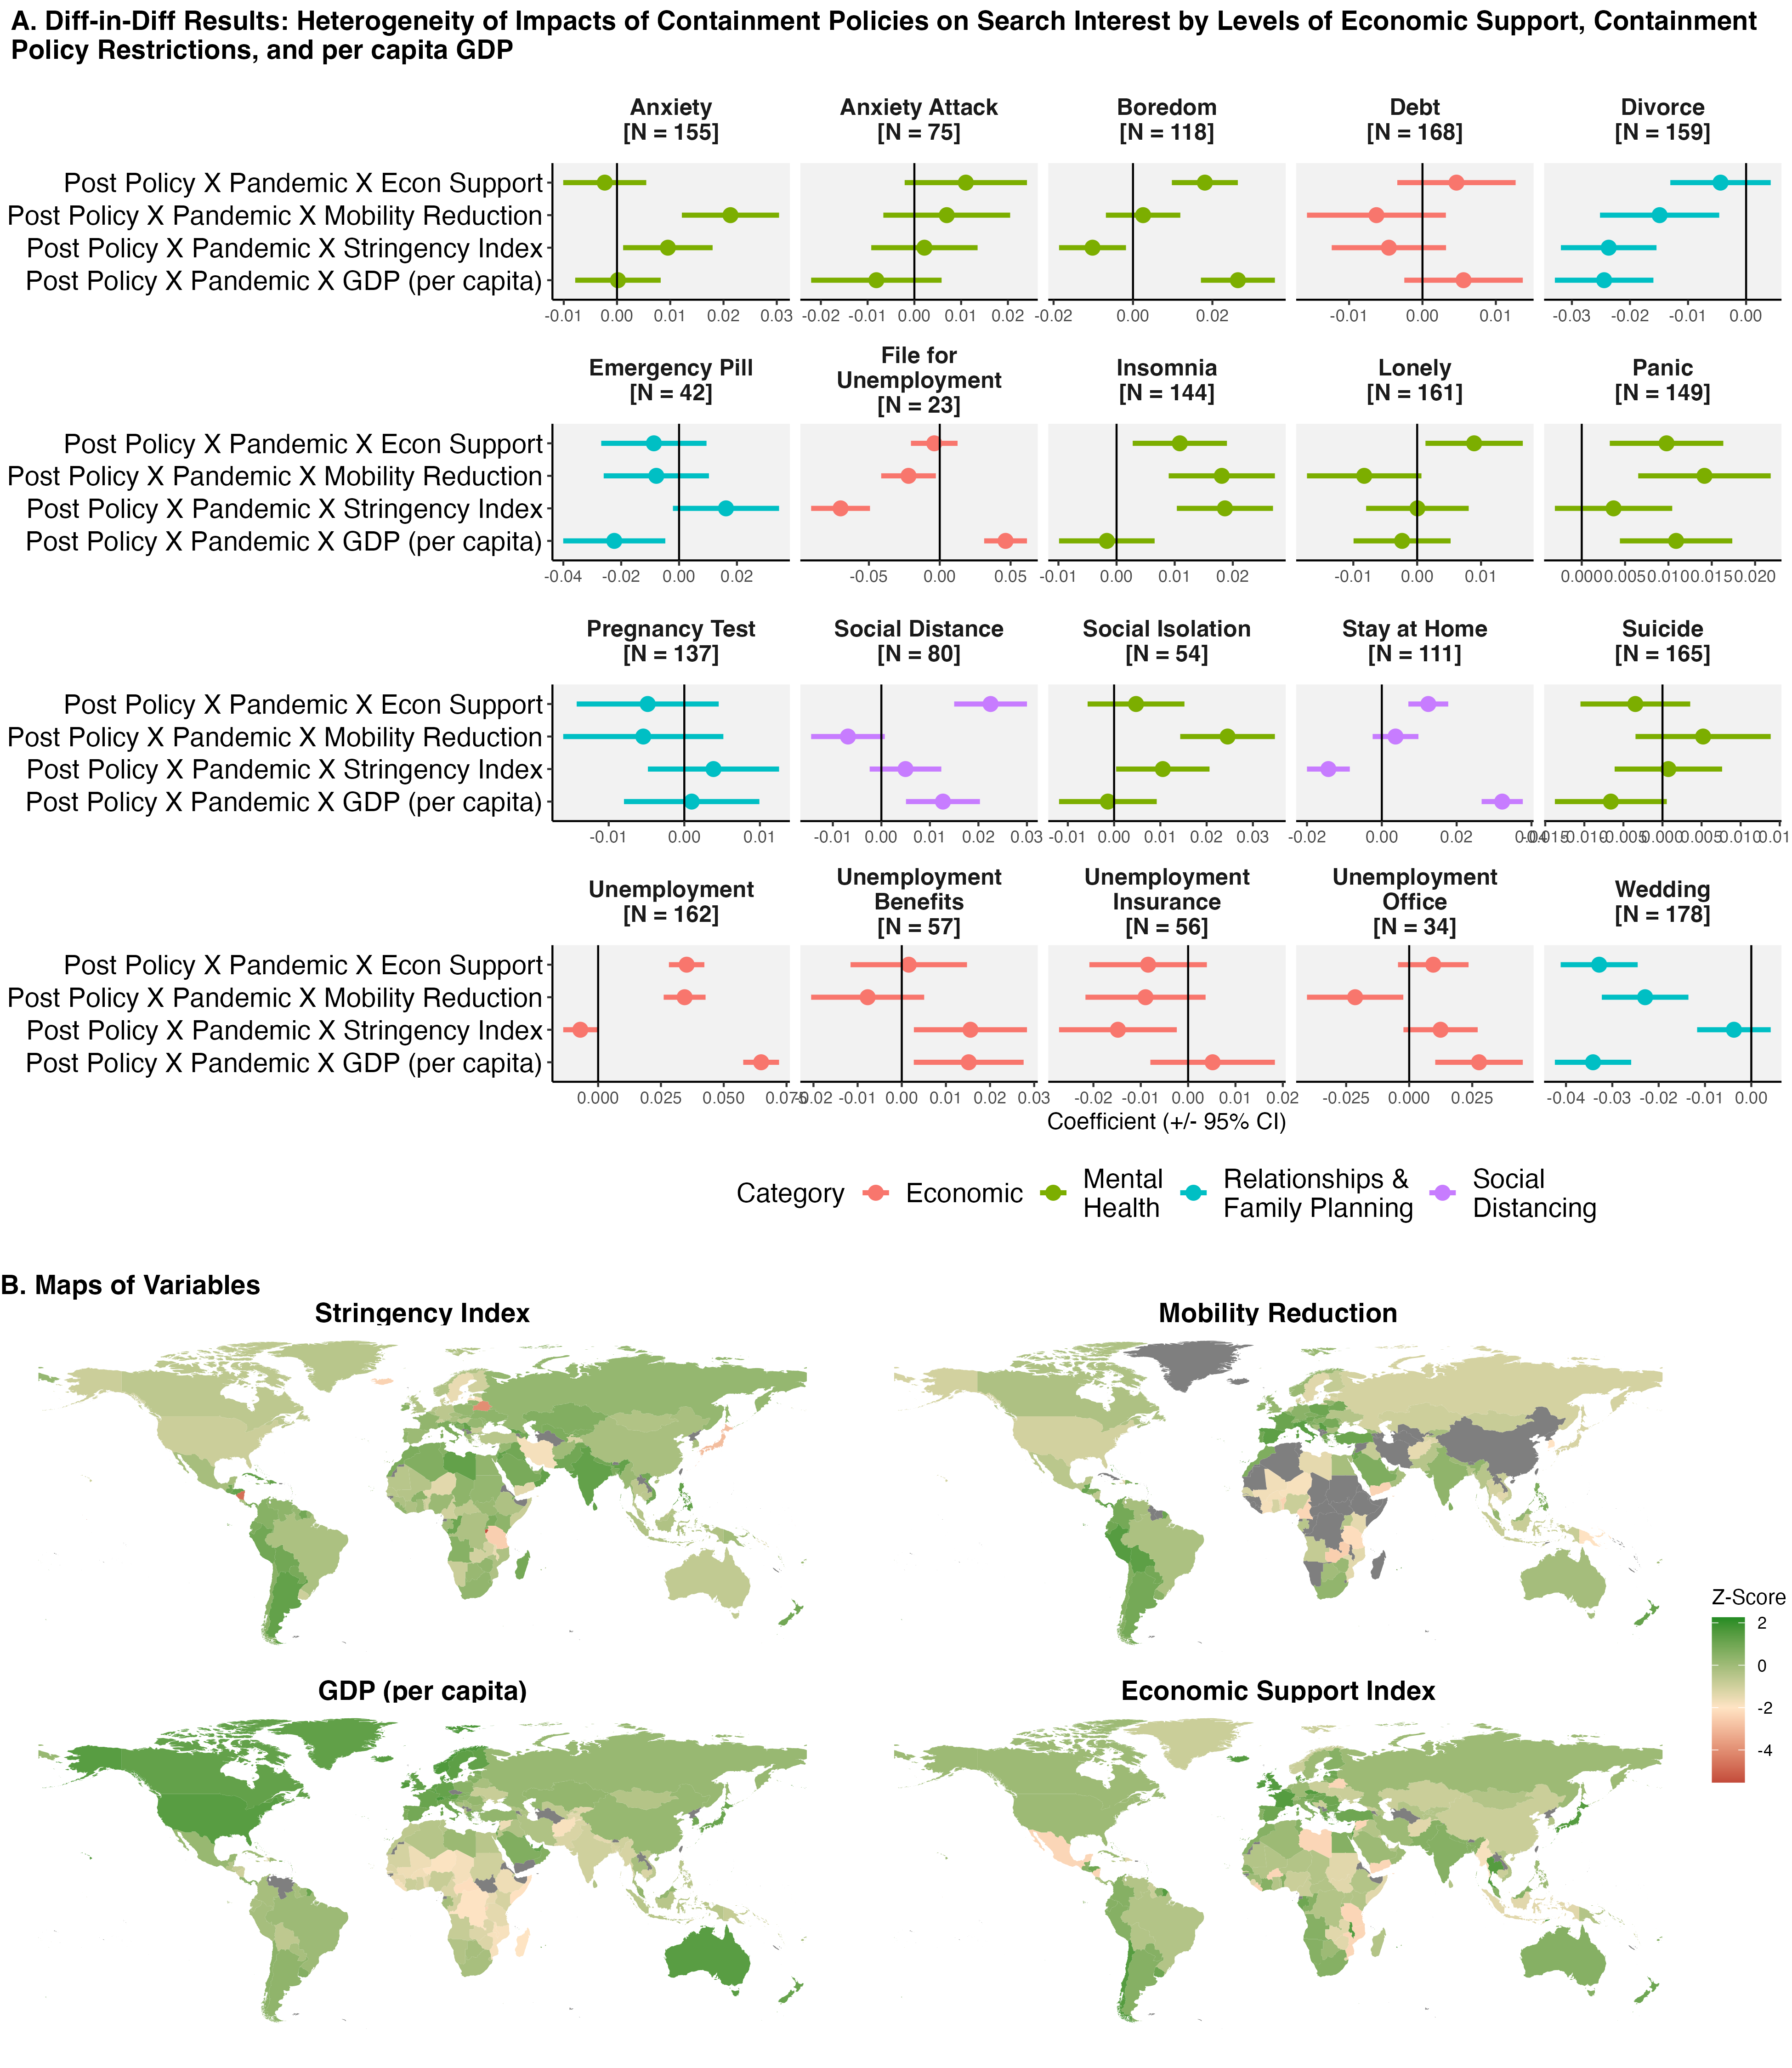
\includegraphics[width=0.85\textwidth]{figures/did_interact_map_180.png}
    \caption{\textcolor{black}{Association of COVID-19 policies with search interest: difference-in-differences results that explore heterogeneity of results across containment policy restrictiveness, economic support, and GDP per capita. Each coefficient comes from a separate regression. The stringency index comes from the University of Oxford COVID-19 Government Response tracker, a composite measure of the restrictiveness of policy measures. Mobility reduction comes from Google COVID-19 Community Mobility Reports, which measure the percent change in mobility relative to pre-pandemic levels. Per capita GDP comes from the World Bank's World Development Indicators; we use log per capita GDP. The Economic Support index from the Oxford COVID-19 Government Response tracker, which measures the extent of economic support across metrics such as income support and debt relief. We standardize all variables into z-scores---having a mean of zero and standard deviation of one. `N' indicates the number of countries with available data. Maps produced using R, version 4.2.2 (\url{https://www.r-project.org/}); data for country boundaries come from Natural Earth (\url{https://www.naturalearthdata.com/}).}}
    \label{fig:did_interact_map_180}
\end{figure}

\begin{figure}[H]
    \centering
    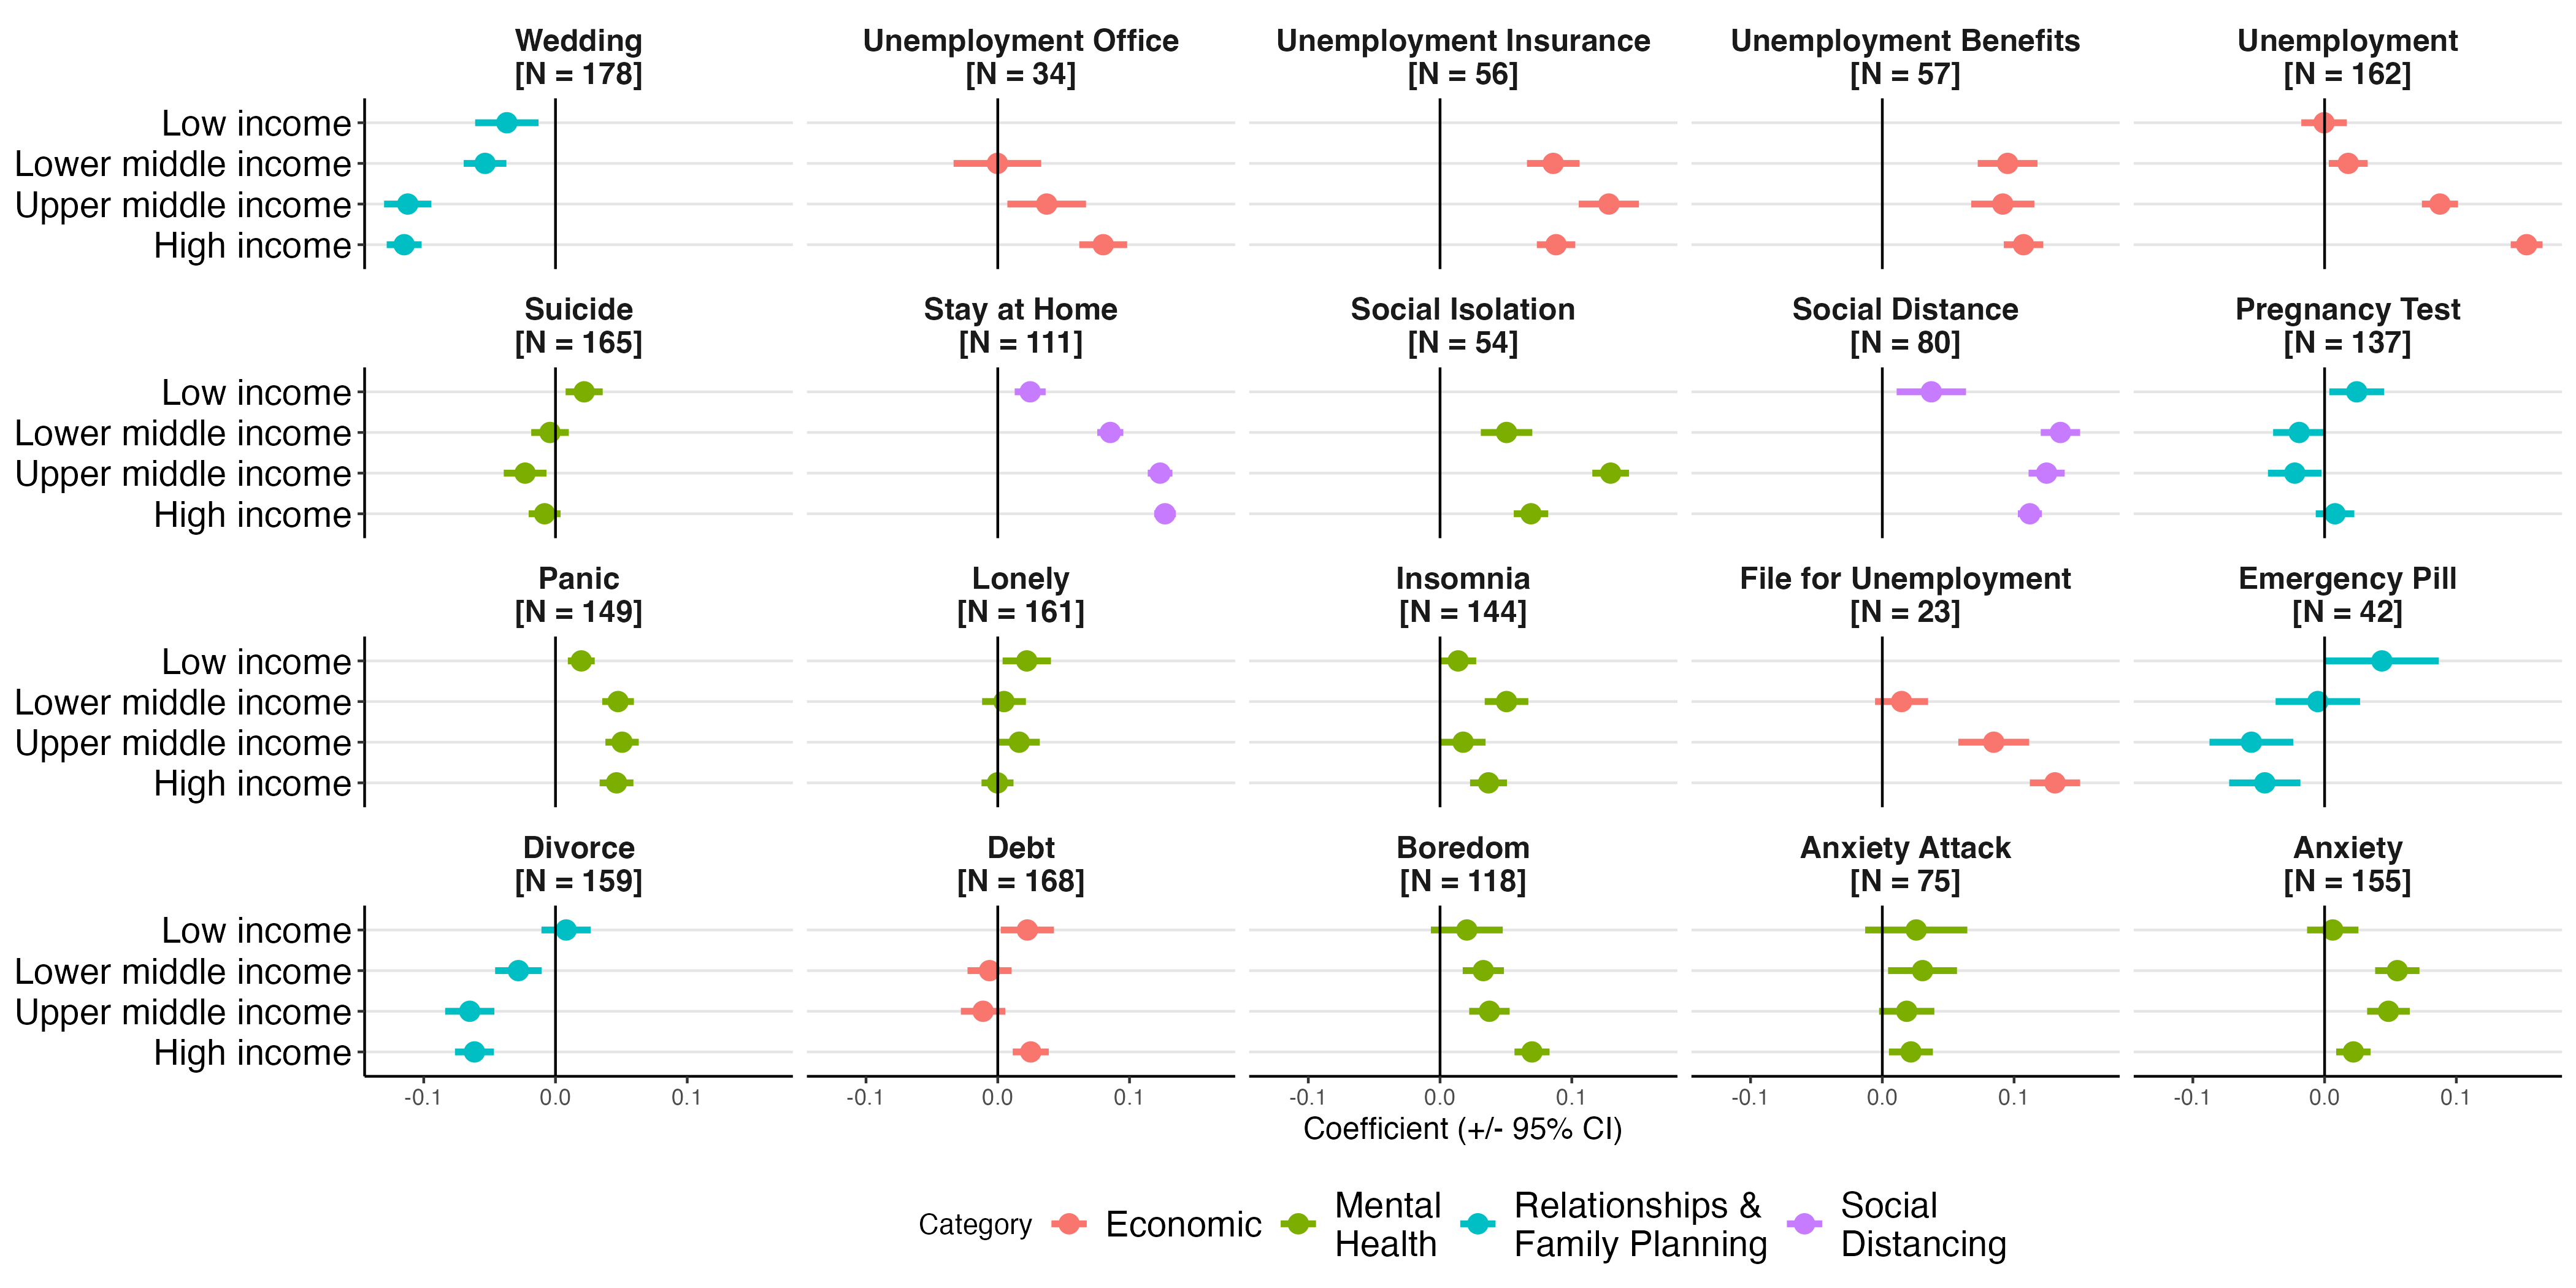
\includegraphics[width=0.85\textwidth]{figures/did_income_180.png}
    \caption{\textcolor{black}{Association of COVID-19 policies with search interest: difference-in-difference results pooling countries by income level. Point estimates and 95\% confidence intervals are shown. `N' indicates the number of countries with available data.}}
    \label{fig:did_income_180}
\end{figure}

% --------------------------
\newpage
\bibliographystyle{plain}
\bibliography{references}
\end{document}



